% =============================================================================
%  SŌKYŪ-Ō SOBA ZENSHŪ — Complete Collected Works on Markets by Master Sōkyū
%  First English Translation
%
%  Original text: 本間宗久 (Honma Sōkyū / Honma Kosaku)
%  Annotated by: 早阪二菊 / 早坂豊藏 (Hayasaka Nikiku / Hayasaka Toyozō)
%  Source: NDL 古典籍OCR-Lite of the Meiji 43 (1910) Shingidō edition
%
%  Edited and produced by Zach Booth
%  Translated with AI assistance (Claude, Anthropic)
%
%  Compiled with XeLaTeX
%  Second volume in the Soba Hidensho series
% =============================================================================

\documentclass[10pt, openany]{book}

\usepackage[
  papersize={6in,9in},
  margin=0.75in,
  inner=0.85in,
  outer=0.65in,
  top=0.8in,
  bottom=0.8in
]{geometry}

\usepackage{fontspec}
\setmainfont{NotoSerif}[
  Path={/Users/grob/Library/TinyTeX/texmf-dist/fonts/truetype/google/noto/},
  Extension=.ttf,
  UprightFont=*-Regular,
  BoldFont=*-Bold,
  ItalicFont=*-Italic,
  BoldItalicFont=*-BoldItalic,
]
\setsansfont{NotoSans}[
  Path={/Users/grob/Library/TinyTeX/texmf-dist/fonts/truetype/google/noto/},
  Extension=.ttf,
  UprightFont=*-Regular,
  BoldFont=*-Bold,
  ItalicFont=*-Italic,
  BoldItalicFont=*-BoldItalic,
]
\IfFontExistsTF{Noto Serif CJK JP}{%
  \newfontfamily\japanesefont{Noto Serif CJK JP}[AutoFakeBold=2.5]%
}{%
  \newfontfamily\japanesefont{Hiragino Mincho ProN}[AutoFakeBold=2.5]%
}
\newcommand{\jp}[1]{{\japanesefont #1}}

\usepackage{graphicx}
\usepackage{xcolor}
\usepackage{titlesec}
\usepackage{fancyhdr}
\usepackage{enumitem}
\usepackage{booktabs}
\usepackage{microtype}
\emergencystretch=1em
\usepackage{hyperref}
\usepackage{float}
\usepackage{setspace}
\usepackage{lettrine}
\usepackage{parskip}
\usepackage{needspace}
\usepackage{mdframed}

% --- Series color scheme (matches Sanen Kinsen Hiroku) ---
\definecolor{chaptercolor}{HTML}{8B0000}
\definecolor{sectioncolor}{HTML}{333333}

% --- Sōkyū's original text: warm parchment box with dark-red left bar ---
\definecolor{sokyubg}{HTML}{F5EDE0}
\definecolor{sokyubar}{HTML}{8B0000}
% Sōkyū's text boxes: allow page breaks but style them cleanly.
% The needspace in \article{} ensures short boxes don't orphan;
% long boxes split with continued background + left bar.
\newmdenv[
  topline=false,
  bottomline=false,
  rightline=false,
  linewidth=3pt,
  linecolor=sokyubar,
  backgroundcolor=sokyubg,
  innerleftmargin=12pt,
  innerrightmargin=12pt,
  innertopmargin=8pt,
  innerbottommargin=8pt,
  skipabove=10pt,
  skipbelow=10pt,
  splittopskip=8pt,
  splitbottomskip=8pt,
  needspace=5\baselineskip,
]{sokyubox}

% --- Editorial note box (same as Sanen series) ---
\definecolor{editorbg}{HTML}{F5F2EB}
\definecolor{editorbar}{HTML}{BBBBBB}
\newmdenv[
  topline=false,
  bottomline=false,
  rightline=false,
  linewidth=2pt,
  linecolor=editorbar,
  backgroundcolor=editorbg,
  innerleftmargin=10pt,
  innerrightmargin=10pt,
  innertopmargin=6pt,
  innerbottommargin=6pt,
  skipabove=8pt,
  skipbelow=8pt,
]{editorbox}
\newenvironment{editorialnote}{%
  \begin{editorbox}\small\textit{Editor's note:}\enspace}{\end{editorbox}}

% --- Heading styles ---
\titleformat{\chapter}[display]
  {\normalfont\Large\bfseries\color{chaptercolor}}
  {\chaptertitlename\ \thechapter}{12pt}{\LARGE}
\titlespacing*{\chapter}{0pt}{-20pt}{20pt}

\titleformat{\section}
  {\needspace{4\baselineskip}\normalfont\large\bfseries\color{sectioncolor}}
  {\thesection}{1em}{}

\titleformat{\subsection}
  {\needspace{3\baselineskip}\normalfont\normalsize\bfseries\itshape\color{sectioncolor}}
  {\thesubsection}{1em}{}

% Prevent headings and first lines from being stranded at page bottom
\widowpenalties 3 10000 10000 150
\clubpenalties 3 10000 10000 150

% --- Page headers and footers ---
\pagestyle{fancy}
\fancyhf{}
\fancyhead[LE]{\small\itshape S\=oky\=u-\=o Soba Zensh\=u}
\fancyhead[RO]{\small\itshape\leftmark}
\fancyfoot[CE,CO]{\small\thepage}
\renewcommand{\headrulewidth}{0.4pt}

\renewcommand{\chaptermark}[1]{\markboth{#1}{}}

% --- Macros ---
\newcommand{\tn}[1]{\footnote{\textit{Translator's note:} #1}}
\newcommand{\jt}[2]{\jp{#1} (\textit{#2})}
% Article heading macro: \article{N}{English Title}
% Ensures enough space for heading + start of sokyubox
\newcommand{\article}[2]{%
  \needspace{8\baselineskip}%
  \section*{Article #1: #2}%
  \addcontentsline{toc}{section}{Article #1: #2}%
  \markright{Article #1: #2}%
}

% Commentary label for Hayasaka's annotations
% Full form on first use, short form thereafter
\newif\iffirstcommentary
\firstcommentarytrue
\newcommand{\commentary}{\needspace{3\baselineskip}\medskip\noindent%
  \iffirstcommentary
    {\small\scshape Commentary} (\jp{釋}, \textit{Shaku}):\enspace%
    \global\firstcommentaryfalse
  \else
    {\small\scshape Commentary}:\enspace%
  \fi}

% --- Hyperref ---
\hypersetup{
  colorlinks=true,
  linkcolor=chaptercolor,
  urlcolor=blue!60!black,
  pdftitle={Sōkyū-ō Soba Zenshū: Complete Collected Works on Markets by Master Sōkyū},
  pdfauthor={Edited by Zach Booth; translated with AI assistance (Claude Opus 4.6, Anthropic)},
}
\pdfstringdefDisableCommands{\def\jp#1{}}
\pdfstringdefDisableCommands{\def\jt#1#2{#2}}

% =============================================================================
\begin{document}

% --- Half-title ---
\thispagestyle{empty}
\begin{center}
\vspace*{2.5in}
{\Large\itshape S\=oky\=u-\=o Soba Zensh\=u}\\[0.5em]
{\large Complete Collected Works on Markets\\by Master S\=oky\=u}
\vfill
\end{center}
\newpage\thispagestyle{empty}\mbox{}\newpage

% --- Title page ---
\thispagestyle{empty}
\begin{center}
\vspace*{1in}
{\huge\bfseries\color{chaptercolor} \jp{宗久翁相場全集}}\\[1em]
{\LARGE\bfseries S\=oky\=u-\=o Soba Zensh\=u}\\[0.7em]
{\Large\itshape Complete Collected Works on Markets\\by Master S\=oky\=u}\\[2em]
\rule{3in}{0.5pt}\\[1.5em]
{\large\itshape An Annotated Edition of the\\Rice Trading Teachings of}\\[0.5em]
{\large \jp{本間宗久}}\\
{\normalsize Honma S\=oky\=u (1717--1803)}\\[1.5em]
{\normalsize Collated, annotated, and edited by}\\[0.3em]
{\large \jp{早阪二菊}}\\
{\normalsize Hayasaka Nikiku}\\[0.3em]
{\small Meiji 43 (1910) --- Shingid\=o, Tokyo}\\[2em]
\rule{3in}{0.5pt}\\[1.5em]
{\normalsize Edited and produced by Zach Booth}\\[0.3em]
{\small Translated with AI assistance}\\[3em]
\end{center}
\vfill
\newpage

% --- Copyright / attribution (page 1: provenance) ---
\thispagestyle{empty}
~\vfill

\begin{small}
\noindent\textbf{Source Text}\\[0.3em]
\noindent\jp{宗久翁相場全集} (\textit{S\=oky\=u-\=o Soba Zensh\=u})\\
Publisher: Shingid\=o (\jp{信義堂}), Kakigara-ch\=o, Nihonbashi-ku, Tokyo\\
Date: April, Meiji 43 (1910)\\
Collated and annotated by Hayasaka Nikiku (\jp{早阪二菊})\\
Original text by Honma S\=oky\=u (\jp{本間宗久}, also known as Honma Kosaku \jp{本間古作})\\[0.5em]
Digitized by the National Diet Library of Japan\\
OCR: NDL \jp{古典籍OCR-Lite}\\[1em]

\noindent\textbf{Open Source}\\[0.3em]
\begin{sloppypar}\noindent The complete methodology---including
OCR transcription, working translation files, and \LaTeX{} source---is
available at
\url{https://github.com/groverburger/japanese}.
\end{sloppypar}
\end{small}
\newpage

% --- Copyright / attribution (page 2: edition info) ---
\thispagestyle{empty}
~\vfill

\begin{small}
\noindent English translation copyright \textcopyright{} 2026 Zach Booth.
All rights reserved. The \LaTeX{} source and methodology are released
under CC BY-NC-SA 4.0.\\[1em]

\noindent\textbf{About This Edition}\\[0.3em]
\begin{sloppypar}\noindent This is the first English translation of the
\textit{S\=oky\=u-\=o Soba Zensh\=u}. The original is a Meiji-era
(1910) annotated edition of Honma S\=oky\=u's rice-trading writings,
compiled by Hayasaka Nikiku from the Honma family's autograph manuscript
and various circulating hand-copies. The translation was produced in two
mechanically-separated stages:\end{sloppypar}\par\vspace{0.4em}
\begin{sloppypar}
\noindent\textit{1. Transcription.} The printed Meiji edition was
passed through NDL~\jp{古典籍OCR-Lite}, a specialist OCR toolchain
released by Japan's National Diet Library. This step is purely
mechanical: the model reads pixels, not meaning.
\end{sloppypar}\vspace{0.3em}
\noindent\textit{2. Translation.} The OCR output was then rendered
into English with AI assistance (Claude Opus~4.6, Anthropic), working
from the mechanical transcription and consulting the manuscript images
only to sanity-check OCR artifacts.\\[1em]

\noindent\textbf{How to Read This Translation}\\[0.3em]
\noindent This book has a distinctive two-layer structure. S\=oky\=u's
own words --- the original Edo-period trading instructions --- appear in
\textbf{tinted boxes with a red left border}, presented first in Japanese
and then in English translation. Hayasaka's Meiji-era commentary
(\jp{釋}, \textit{shaku}) follows in regular body text, introduced by
a {\small\scshape Commentary} label. This visual distinction is
editorial: the source text interleaves the two voices without
typographic differentiation. Footnotes marked ``\textit{Translator's
note}'' provide additional historical context.\\[0.5em]

\noindent\textbf{Structure of the Text.}
The front matter comprises a preface by Hayasaka, a brief biography of
S\=oky\=u in classical Chinese, and a description of the Sakata Rice
Exchange's trading customs. The body consists of 158 numbered articles
across two volumes (Upper, 73 articles; Lower, 85 articles), followed by
historical price records. Article lengths vary enormously: some are a
single sentence, others span several pages.\\[0.5em]

\noindent\textbf{On the Missing Page.}
Page~88 of the source is absent from the NDL scan (marked \jp{欠},
``lacking''), taking with it the body text of Lower Volume Articles
67--84. Only the table-of-contents entries survive.
\end{small}
\newpage

% =============================================================================
\thispagestyle{empty}
\tableofcontents
\newpage

% =============================================================================
\chapter*{Translator's Introduction}
\addcontentsline{toc}{chapter}{Translator's Introduction}
\markboth{Translator's Introduction}{}

The \textit{S\=oky\=u-\=o Soba Zensh\=u} (\jp{宗久翁相場全集}), or
``Complete Collected Works on Markets by Master S\=oky\=u,'' is one of
the foundational texts of Japanese market analysis.\tn{The edition
translated here was published in April 1910 (Meiji~43) by Shingid\=o
(\jp{信義堂}) of Tokyo, collated and annotated by Hayasaka Nikiku
(\jp{早阪二菊}). Hayasaka's preface states that the base text is the
Honma family's autograph manuscript, supplemented by dozens of additional
articles from circulating hand-copies.}
It preserves the trading teachings of Honma S\=oky\=u (1717--1803), the
legendary rice speculator of Sakata, Dewa Province, whose methods on the
Osaka D\=ojima and Sakata exchanges are considered among the earliest
systematic approaches to market analysis anywhere in the world.

\section*{Who Was Honma S\=oky\=u?}

Honma S\=oky\=u --- known in his lifetime as Honma Kosaku (\jp{本間古作})
--- was born in 1717 into a farming family in Tagawa district, Dewa
Province (modern Yamagata Prefecture). Adopted into the powerful Honma
merchant house of Sakata, he observed rice price movements for years
before experiencing what the biography in this volume calls a ``sudden,
sweeping enlightenment'' (\jp{一旦豁然有所悟焉}). From that point
forward, his trades on the Sakata exchange were unfailingly profitable.
He later moved to Osaka --- the national center of the rice futures
market --- where he again amassed enormous wealth, and finally to Edo,
where he entered the service of the Rinn\=o-ji-no-miya at Ueno. He died
in 1803 at the age of eighty-seven.

His writings circulated as secret transmission texts (\jp{相場秘伝書},
\textit{s\=oba hidensho}), copied and recopied among traders for
generations. By the Meiji period, these hand-copies had diverged
considerably, prompting Hayasaka's systematic edition.

\section*{The Two Voices}

What makes this text unusual is its two-layer structure. Each chapter
contains two distinct voices:

\begin{enumerate}
\item \textbf{S\=oky\=u's original text} --- terse, oracular,
  imperative. He writes in the voice of a master transmitting secret
  knowledge to a disciple. His sentences are short, his maxims memorable:
  \textit{``At two, close out; at three, fully ripe; at four, it
  turns.''} He teaches by principle, not by explanation.

\item \textbf{Hayasaka's commentary} (\jp{釋}) --- analytical,
  discursive, pedagogical. Writing three centuries later, Hayasaka
  unpacks S\=oky\=u's compressed instructions for a modern audience. He
  gives hypothetical examples, cross-references other chapters, cites
  Western economists (including David Ricardo), and explains the
  now-vanished customs of the Sakata Rice Exchange.
\end{enumerate}

In this edition, S\=oky\=u's words appear in tinted boxes to make the
distinction immediately visible. The reader can follow S\=oky\=u's
teachings as a continuous thread, or read each chapter complete with
Hayasaka's gloss.

\section*{The Three-Position Tradition}

\begin{sloppypar}
At the heart of S\=oky\=u's method stands the \textit{sanmi no den}
(\jp{三位の傳}), the ``Three-Position Tradition.'' Its central formula
--- \jp{二ツ仕廻、三ツ十分、四ツ轉じ}, ``At two, close out; at three,
fully ripe; at four, it turns'' --- encodes a theory of market rhythm:
\end{sloppypar}
trends exhaust themselves in predictable stages. When a market has moved
``two'' (whatever the unit of observation), it is time to close; at
``three,'' the move is fully mature; at ``four,'' reversal is imminent.

S\=oky\=u supplements this with the Heavenly Stems calendar system
(\jp{十干}), in which each month is assigned a celestial stem, and the
first four stems (kinoe through hinoto) signal rising markets while the
remaining six signal falling. Whether this calendar method holds
predictive power is beside the point for the modern reader; what matters
is the underlying logic of cyclicality, exhaustion, and contrarian
discipline that pervades every chapter.

\section*{Reading This Book}

The text rewards both linear and selective reading. Articles~1--15 of
the Upper Volume lay the philosophical foundation. The famous maxims
--- ``leap into the fire,'' ``plunge into the sea,'' ``the lamp burns
brightest before it dies'' --- appear in Articles~3, 4, and~35.
The practical trading rules cluster in Articles~30--50 of each volume.
The calendar and almanac articles (Lower Volume, Articles~27--36) are
the most culturally remote but offer a window into Edo-period
cosmological thinking about markets.

The Lower Volume's Article~48 contains perhaps the most celebrated
maxim in all of Japanese trading literature:

\begin{center}
\textit{``What seems too late is still early;\\
what seems still early is already too late.''}
\end{center}

\vspace{1em}

\begin{flushright}
\textit{--- Zach Booth, 2026}
\end{flushright}

% =============================================================================
%  FRONT MATTER: Preface, Notes, Biography, Trading Customs
% =============================================================================
\chapter{Preface and Front Matter}
\markboth{Preface and Front Matter}{}

\section{Preface (\jp{緒言})}

The posthumous writings of Master S\=oky\=u are a book of lofty insight
and striking perception, exhaustively explicating the methods by which
one penetrates the subtleties of the market, leaving nothing to be
desired. How fitting, indeed, that the master achieved such great
success. Yet the original manuscript in the master's own hand has been
kept under lock in the family's treasury, not easily seen by outsiders.
Meanwhile, the hand-copies circulating in the world are rife with
scribal errors --- characters mistaken one for another, corruptions
multiplying with each transcription. This not only does violence to the
true meaning of the master's teachings but risks leading future students
astray.

Troubled by this state of affairs, we earnestly petitioned the Honma
family and obtained permission to transcribe the master's autograph
manuscript. We further collated it against the various hand-copies in
circulation, thereby supplementing several dozen additional articles.
Moreover, where the text employs trade jargon or presents difficult
passages, we have appended individual annotations to elucidate the
meaning. The resulting work we have titled \textit{S\=oky\=u-\=o Soba
Zensh\=u}. Now that it has gone to press, we offer these few words at
the head of the volume to make clear its provenance.

\begin{flushright}
\textit{April, Meiji 43 (1910). Hayasaka Yutaka.}
\end{flushright}

\section{Annotator's Notes (\jp{凡例})}

\textbf{One.} This book takes as its base text the autograph manuscript
held in secret by the master's family, corrected and supplemented by
reference to the hand-copies in circulation, with annotations added in
an effort to bring out the true meaning. Yet given the annotator's own
limitations, we fear we may fail to convey even a tenth of the master's
true intent. Particularly when it comes to the subtle art of market
maneuvering (\jt{駈引}{kakehiki}) and the rhythm of trading --- these
are matters that no brush or tongue can fully exhaust. The reader is
advised to seek the meaning beyond the words.

\textbf{Two.} All dates recorded in this book follow the lunar calendar
(\jt{太陰暦}{taiin-reki}). Wherever the text says ``this region''
(\jt{當地}{t\=ochi}), it refers to the Sh\=onai district
(\jp{荘内地方}).

\textbf{Three.} The principles in this book may be applied in any
region, but since the master based his arguments on the Sh\=onai
district, a clear understanding of the text requires the reader first to
comprehend the trading customs of the Sh\=onai rice merchants. This is
precisely why we have included the customs of the former Sakata Rice
Exchange (\jt{酒田米會所}{Sakata Kome Kaisho}) at the head of the
volume.

\textbf{Four.} Anyone who wishes to grasp the subtle art of futures
maneuvering (\jt{期米駈引}{kimai kakehiki}) must read this book through
again and again, many times over. Do so, and in time one will naturally
come to distinguish strength from weakness in the market and master the
art of maneuvering. Above all, while one holds an open position, one
must never neglect this reading --- for to do so is to grow careless in
one's attention to the market.

% =============================================================================
%  BIOGRAPHY
% =============================================================================
\chapter{A Brief Biography of Master Honma S\=oky\=u}
\markboth{Biography of Honma S\=oky\=u}{}

\begin{editorialnote}
The biography that follows is written in classical Chinese
(\textit{kanbun}), the formal literary language of Meiji-era scholarly
prose. It was composed by Hayasaka as a prefatory tribute.
\end{editorialnote}

The master's common name was Kosaku (\jp{古作}). He belonged to the
Honma (\jp{本間}) clan, the great landholding family of Dewa Province,
renowned throughout the realm as foremost farmers. In later years the
master took up residence at Negishi in Edo, and thus the world knew his
line as ``the Negishi Honma.'' By nature quick and spirited, striking in
his perceptions, he possessed an uncanny ability to read the signs of
the market. In his advances and retreats he never erred by so much as a
hair's breadth, and through the buying and selling of rice he amassed
enormous wealth. That the Honma house today stands as the richest in all
Japan is, of course, largely owing to the great efforts of its restorer
Shir\=osaburō (\jp{四郎三郎}) --- yet the master's supporting
contribution was by no means small. To relate the master's career, we
must first trace the origins of the main Honma family's fortune.

\subsection*{The Founding of the Honma Fortune}

The Honma were originally surnamed Sat\=o. Their ancestor, a man called
Ky\=ushir\=o (\jp{久四郎}), was a native of Sado. More than two hundred
and fifty years ago he came to Sakata, destitute, and entered service as
a retainer of a certain Honma household. This Honma family had lived in
Sakata for generations, operating a shipping agency
(\textit{kaisen don'ya}), and was counted among the town's leading
houses. Ky\=ushir\=o, quick and diligent by nature, devoted himself
faithfully to his duties and quickly earned his master's deep trust,
before long being elevated to chief steward.

It happened that the head of the Honma house was imprisoned on some
charge, and he entrusted all affairs to Ky\=ushir\=o. Fearing above all
to betray this trust, Ky\=ushir\=o threw himself into the work --- from
overseeing the entire shop to receiving its customers, he shouldered
every responsibility himself --- and in the end preserved the house's
reputation undiminished. When the master's innocence was established and
he returned home, he found his assets undiminished and his credit intact
as before. Greatly pleased, he rewarded Ky\=ushir\=o's service by
bestowing upon him the Honma name and establishing a branch house under
his charge. This was the founding ancestor of the present-day Honma
fortune.

The lands of Sh\=onai enjoyed bountiful harvests year after year, and
the price of rice was deeply depressed. Ky\=ushir\=o privately reasoned:
though the paddies now yield abundantly and rice is cheap, when autumn
passes into winter and buyers come competing, the price must surely
rise. He committed his entire resources to purchasing spot rice
(\jt{正米}{sh\=omai}). Sure enough, merchants from the various
provinces came rushing to buy; demand outstripped supply, and the price
leapt upward. Ky\=ushir\=o seized the moment to sell, and in a single
stroke reaped enormous profit.

\subsection*{S\=oky\=u's Enlightenment}

Master S\=oky\=u was born in the second year of Ky\=oh\=o (\jp{享保二年},
1717) in Niibori village, Tagawa district, Dewa Province. As a child he
was adopted into the Honma house. When the second-generation head died
and the young Shir\=osaburō was still a child, S\=oky\=u assumed
temporary charge of the household affairs and took up residence at
Shimogura (\jp{下藏}) --- a corner of Sakata's Funaba-ch\=o where the
Honma family's warehouses stood.

The master reasoned: anyone who would grow rich through commerce must
choose a trade with broad distribution channels and smooth transactions.
The lands of Ry\=ou (\jp{兩羽}) stretch across tens of \textit{ri} of
fine paddies, and Sakata possesses a rice exchange where large and fluid
transactions take place. Surely the trade to pursue is the rice trade.

From that time he immersed himself in the principles governing the rise
and fall of rice prices, observing with a broad eye the shifts in market
sentiment (\jt{人氣}{ninki}). After several years, one day he
experienced a sudden, sweeping enlightenment. From then on, whenever he
traded rice --- when he sold, prices fell; when he bought, they rose ---
there was nothing he undertook that did not yield profit. In short order
he accumulated tens of thousands of gold pieces.

He later traveled to Osaka --- the foremost rice market in all Japan ---
where he invariably seized the initiative before others could act; the
brilliance of his dealings left traders of many generations gaping in
astonishment. He then proceeded to Edo, entered the service of the
Rinn\=o-ji-no-miya at Ueno, and built a residence at Negishi. In old
age he transferred the household to his adopted son Inoshir\=o
(\jp{猪四郎}). He died on the last day of the eighth month of Ky\=owa~3
(\jp{享和三年}, 1803) at his Negishi residence, at the age of
eighty-seven. He was buried at Zuitoku-ji (\jp{隨徳寺}) in Shitaya
Sakamoto-ch\=o.

\subsection*{S\=oky\=u and Zenb\=e}

Few anecdotes of the master's life survive. Only this is told: while the
master still lived at Shimogura in Sakata, there was a rice-pounder
named Zenb\=e (\jp{善兵衛}) who had speculated in rice, misjudged the
market, and very nearly lost his entire fortune. The master sent a man to
observe his situation. The report came back: he works bare to the waist,
pounding rice, drenched in sweat. The master judged: this man can be
helped. He summoned Zenb\=e and asked: ``I hear you owe several hundred
gold pieces, yet you pound only two or three mortars of rice a day. How
do you expect to recover?'' Zenb\=e answered: ``I have a wife and
children, and I cannot let them go hungry for even a single day. The
rice-pounding merely sustains us. As for recovery --- I have other hopes
for the future.'' The master said: ``I hear that you bought and lost. If
you had capital now, would you buy or sell?'' Zenb\=e replied: ``I would
still buy.'' The master said: ``Good. I shall give you the capital. Buy
at once and do not hesitate.'' Zenb\=e bought heavily, the price surged,
and he recovered his fortune entirely.

S\=oky\=u once said to Zenb\=e: ``The rice traders of Sakata are all
blind to the art of reading the moment. I now entrust you with my
strategy'' --- and he produced a single volume and gave it to him. That
book is this book. Its value, then, need hardly be stated.

The master was born into a farming household. Through innate acuity and
many years of practical experience he secured his success, enlarged the
main family's fortune, and raised himself to the standing of a wealthy
commoner ranked above the samurai class. More than a hundred years have
passed since his death, yet he is still revered by rice traders. Can
this be mere accident?

% =============================================================================
%  TRADING CUSTOMS
% =============================================================================
\chapter{Trading Customs of the Sakata Rice Exchange}
\markboth{Sakata Rice Exchange}{}

In setting out the trading customs of the Sakata Rice Exchange
(\jt{酒田米會所}{Sakata Kome Kaisho}), one must first say a word about
Sakata's geography. Its western expanse faces the Sea of Japan and lies
at the mouth of the Mogami River (\jp{最上河}), giving it great
advantage for water transport. The various lords whose domains border the
Mogami --- their tribute rice and domain-tax rice as well as merchants'
private stocks --- all of this was customarily shipped to this port and
traded at the exchange's market. Rice from the Mogami, Yonezawa
(\jp{米澤}), and Sh\=onai regions converged on Sakata in quantities
that at times exceeded several hundred thousand \textit{koku}.

Merchants from Nagato, Izumo, Iwami, Shikoku, Kaga, Noto, and the
Matsumae region each loaded their local products onto traditional sailing
vessels (\textit{wasen}), came to sell their goods, and purchased rice to
carry home.

As is common in northern regions, from around the tenth month through the
second and third months of the following spring, fierce northerly winds
made navigation difficult. Despite fewer ships entering port, rice
continued to flow out in volume, keeping the price low. Merchants from
the various provinces therefore came in what was called ``winter buying''
(\jt{冬買}{fuyugai}) --- purchasing spot rice and waiting for the first
ships of spring to export it. The spot-rice trade thus flourished
enormously, and the need for a rice exchange arose. The institution
called the \textit{Hozakata} (\jp{歩座方}), the exchange proper, dates
its founding to some hundred and forty or fifty years before the time of
writing.

\subsection*{Sh\=onai Rice Certificates}

Tracing their origin: in Genna~8 (\jp{元和八年}, 1622), when Sakai
Tadakatsu (\jp{酒井忠勝}) was granted the Sh\=onai domain, he
vigorously promoted agriculture and land reclamation, and rice production
increased year by year. A chief retainer named Shibaya Buemon
(\jp{柴谷武右衛門}) vigorously reformed the domain's finances: he
established domain granaries in both Sakata and Tsuruoka (\jp{鶴岡}),
requiring all tribute rice to be delivered by the tenth month of each
year. Against these deposits, rice certificates (\textit{kome-fuda}) were
issued. Samurai stipends were all paid in these certificates, and rice
sold to merchants was likewise transacted through them. The certificates
could be redeemed at any time for actual rice at the granary. The domain
government supervised the system strictly while permitting the
certificates to circulate freely on the market, treated the same as
actual rice. Trading grew more vigorous with each passing year.

\subsection*{The Founding of the Exchange}

The founding of the Sakata Rice Exchange originated in the trading of
these rice certificates. The certificates possessed several key
advantages: uniform quality, year-long redemption, and transfer by paper
alone without physical inspection. Merchant ships purchased certificates
through wholesalers in great numbers. Among the buyers were speculators
(\jt{思惑人}{omowaku-nin}) who purchased when prices were low and sold
when the market rose. As trading grew ever more active, the wholesalers
agreed to establish a common marketplace. This was the origin of the
Sakata Rice Exchange.

\subsection*{Key Exchange Terms}

\textbf{The November Contract} (\jt{霜月限}{shimotsuki-giri}): the
November delivery month, in which the contract rice is new-crop rice.
Trading typically opened around the middle of the sixth month.

\textbf{Tawara-up and tawara-down} (\jp{何俵上げ / 何俵下げ}): under
the domain's system, rice prices were quoted as so-many bales
(\jt{俵}{tawara}) of five-\textit{to} capacity per ten \textit{ry\=o}.
One ``lot'' (\jp{一枚}) was defined as one hundred \textit{ry\=o} worth.

\textbf{Margin calls} (\jt{落引}{ochibiki}): the forfeit-or-extend
decision on deposited margin money. The threshold varied with periodic
revisions to the exchange rules: sometimes twenty tawara of price
movement, sometimes forty. Under the exchange's system, profit-and-loss
settlement could not be conducted until the contract month arrived. A
margin call against one's position operated the same as an ordinary new
trade.

% =============================================================================
%  UPPER VOLUME
% =============================================================================
\part{Upper Volume (\jp{上卷})}

\chapter*{}
\vspace{-4\baselineskip}
\markboth{Upper Volume}{}

\article{1}{The Initial Entry}

\begin{sokyubox}
{\small\itshape\color{sokyubar} \jp{第一章\quad 米商は踏出大切の事}}

\medskip
In the rice trade, the initial entry (\jt{踏出し}{fumidashi}) is of the
utmost importance. When the entry is poor, one will invariably come to
grief. One must not rush into a trade; to rush is the same as a poor
entry. Whether buying or selling, when the impulse seizes you that today
is the only chance, wait three days. This is the Tradition.

Consider well the oscillation of the rice market, weigh the position of
the ceiling (\jt{天井}{tenj\=o}) and the floor (\jt{底}{soko}), and
only then trade. This is the Three-Position Tradition
(\jt{三位の傳}{sanmi no den}). Until the floor price has emerged, wait
for months on end --- consider the moment when the opportunity aligns,
and then trade.
\end{sokyubox}

\commentary
This is the general preface to Master S\=oky\=u's market method. The
hundred and several dozen articles that follow may all be regarded as
detailed elaborations of this opening statement.

The ``initial entry'' means the moment of committing to a trade. When one
hesitates --- shall I sell, or shall I buy? --- and vacillates between
the two, one enters the trade like a general whose strategic calculations
are already deficient before the battle begins.

To fix one's assessment requires above all that one empty one's mind and
calm one's spirit. It is for this reason that Master S\=oky\=u built a
Zen meditation room behind his house and entered a state of contemplative
absorption (\textit{sanmai}). Yet when we market traders attempt to fix
our assessment, there are demons that seek to cloud the mirror of our
judgment. What are these demons? They are the spirit of haste.

\textit{First:} the haste to profit --- when one borrows money at high
interest and, compelled by the repayment deadline, forces oneself to find
an opportunity where none exists.

\textit{Second:} the envy of another's success --- so-called ``jealousy
buying'' or ``jealousy selling.''

\textit{Third:} the fury of repeated failure --- when one trades
recklessly out of frustration. Such madness is best cured by sitting in
Zen meditation and driving out the demon.

\textit{Fourth:} the conviction that today is the only chance. This is
no demon at all; it is perfectly reasonable. And yet --- experience shows
that what we take for a true opportunity is often a false one wearing a
mask. Therefore, wait three days. Suppress the impulse to rush, calm
oneself, and consider: is this a trending market (\jt{伸相塲}{nobi
s\=oba})? A consolidating market (\jt{保合}{mochai})? Or a range-bound
market (\jt{通相塲}{kayoi s\=oba})? Then weigh the crop conditions, the
volume of old rice, the quality of the wheat harvest, the movements of
the major players; determine whether the current price stands at the
ceiling, the floor, or a middle level; and only when one's conviction
rings true within one's breast should one commit. It is never too late.

\begin{sokyubox}
{\small\itshape\color{sokyubar} Article 1 (continued)}

\medskip
``One must not rush a trade'' means: watch for the ceiling price and the
floor price. ``The initial entry is of the utmost importance'' means:
what emerges often lies beyond what one expected. When one knows the
ceiling and the floor, one trades profitably and without loss. When a
trade is profitable, resist greed; use a hundred-tawara rise as the
benchmark and take profits. Close the trade and rest for forty or fifty
days. ``To rest'' means: to watch for the floor price. Consider all sides
carefully and put this into practice.
\end{sokyubox}

\commentary
The ceiling typically rises more than a hundred tawara above the floor.
Using this hundred-tawara measure as the standard, one can gauge whether
a ceiling or floor is forming. In most cases, a hundred-tawara swing
marks the ceiling or floor; when one sees the signs, one should promptly
take profit. After closing the trade, withdraw and rest quietly for forty
or fifty days, and wait for the next ceiling or floor to appear.

This instruction to rest for forty or fifty days after closing a trade is
indeed golden counsel. One can ride success and increase one's positions,
but to take profit and then \textit{rest} --- this is what is truly
difficult. Looking at the world's failures, eight or nine out of ten come
from traders who pile on more positions heedless of the extremity of the
price, only to be caught by the reversal in sentiment and suffer sudden,
catastrophic loss. This is why the master returned again and again to
this admonition.

% --- Chapter 2 ---
\article{2}{Monthly Rhythms in a Falling Market}

\begin{sokyubox}
{\small\itshape\color{sokyubar} \jp{第二章\quad 下相塲月頭強く月末弱き事}}

\medskip
In a falling market, rice is strong at the opening of the month and
declines through the twenty-ninth and thirtieth. In a rising market's
range-bound oscillation, the month opens weak and the end of the month is
strong, with a sharp upward thrust. Sell positions held through the fifth
month may be carried, at one's discretion, through the twenty-ninth
before closing. But any sell position in the sixth month must be closed
cleanly (\textit{sappari}) by the twenty-first, without exception.
\end{sokyubox}

\commentary
This chapter describes the broad pattern of a falling market after a
ceiling has been reached. Sell positions through the fifth month may be
carried to month-end at one's discretion, but the sixth month brings the
approach of the storm season, when prices tend to rally; therefore sell
positions should be closed as early as possible.

Market sentiment retains the memory of the recent high ceiling price. The
popular feeling of ``prices were high'' is deeply imprinted in people's
minds, and the new low price inspires a vague impulse to buy.
Particularly in a falling market after a ceiling has been struck, each
month opens at a discount to the previous close --- a pattern that tempts
buyers at the month's opening. Prices briefly advance but, lacking any
supporting developments, the market grows heavy. From mid-month into the
latter part, buying thins out and bearish sentiment takes hold.

One point requires particular attention. After two or three months of
month-opening strength followed by month-end weakness, if at month-end
the expected decline fails to materialize and instead the month closes
\textit{high}, take careful note. Such a market sometimes marks the
bottom --- from which prices promptly break upward the following month.

% --- Articles 3 and beyond: assembled from fragments ---
% Note: Article 3 is in upper_03-15.tex (the fragment begins at Article 4,
% but Article 3 "Leaping into the Fire" is also from pages_19-22)
% =============================================================================
%  Upper Volume: Articles 3--15
%  Generated from translation/pages_19-22.md, pages_23-26.md, pages_27-30.md
% =============================================================================

% --- Article 3 is in a prior translation file (pages_15-18.md) ---
% --- This fragment begins at Article 4 ---

\article{4}{On the Resolve to Plunge into the Sea When Everyone Shares the Same Outlook}

\begin{sokyubox}
{\small\itshape\color{sokyubar} \jp{第四章\quad 人も同じ見込の節海中へ飛入る心持の事}}

\medskip
When rice has been falling steadily, when there is no change in the
\jt{上方}{Kamigata} market, when rumours abound that domain rice
(\jt{拂物}{haraimono}) from the provinces and from \jt{最上}{Mogami}
is plentiful, when market sentiment (\jt{人氣}{ninki}) is uniformly
bearish, and when even one's own judgment inclines toward weakness with
no telling how far prices may fall---at precisely that moment, reverse
one's thinking and buy. This resolve requires the spirit of plunging
into the sea. It is an exceedingly unpleasant feeling, yet at that
moment one must not give rise to doubt: buy. This is supremely
profitable. When one expects a decline and the market obliges, it is
easy enough; but when sentiment leans entirely toward decline, the
market perversely rises, and one's calculations avail nothing. The same
applies in the opposite direction. This spirit of plunging into the sea
is the innermost secret.
\end{sokyubox}

\commentary
Mogami refers to the collective name for what is now the Murayama and
Mogami districts. \textit{Haraimono} denotes the official disposal rice
(\jt{御拂米}{ohara-mai}) of the various domains, all of which was
customarily shipped to the port of \jt{酒田}{Sakata} for sale---a point
already noted at the opening of this volume.

The previous chapter explained selling when sentiment has swung
unanimously to the buy side; this chapter explains buying when sentiment
has swung unanimously to the sell side.

When sentiment has tilted entirely toward selling and one's own
sympathies likewise favour the sell side, one must absolutely not sell.
At such a time, one should summon the great courage of one who plunges
into the sea and turn to the buy side. The reason is this: the
phenomenon of unanimously bearish sentiment, seen from one angle, means
that sellers have sold to the absolute limit---the season when
profit-taking (\jt{利喰}{rigui}) must soon emerge is at hand. And since
everyone, without exception, has piled onto the sell side, the subtle
mechanism of a reactive upward turn is already in motion. However, what
the master teaches here applies to cases where both the number of months
and the price level have ripened. It must not be applied when the months
and days are still young. \jt{慈雲齋}{Jiunsai} also says as much:

\textit{``Whether rising or falling, ride the move at five parts or
one-tenth; know that at two- or three-tenths, the market reverses.''}

\textit{``Whether rising or falling, at five parts or one-tenth the ride
is good; past the midpoint, riding is foolish.''}

Together with this chapter, these are worthy admonitions.

% --- Article 5 ---
\article{5}{On Rice That Consolidates from Winter through the First and Second Months}

\begin{sokyubox}
{\small\itshape\color{sokyubar} \jp{第五章\quad 冬より正二月迄持合ふ米の事}}

\medskip
Rice that holds in consolidation (\jt{持合}{mochai}) at the floor price
from mid-winter through the first and second months will, from the third
and fourth months into the fifth and sixth, assuredly rise.
\end{sokyubox}

\commentary
When prices were high the previous year and then declined for three
months or more through January of the following year, this is a market
that fell because the previous year's harvest was abundant, the autumn
supply was ample, and bearish drift (\jt{ダラダラ}{daradara}) was
chanted to exhaustion. With no immediately bullish factors in sight, and
particularly when the winter weather is unobjectionable, sellers appear
early in anticipation of fine equinox weather, and for a time low prices
will persist. This low price often becomes the year's floor price
(\jt{底直段}{soko nedan}). One should therefore consult the chart
(\textit{keisen-hy\=o}), examine the number of months elapsed and the
proportional extent of the decline, weigh these against external
conditions in the broader economy, and resolve to buy. This is what is
called the buying opportunity (\jt{買時機}{kai-jiki}). The reason is
that in such calm, uneventful years, the market has already exhausted
whatever decline it could produce. Even at the equinox---a time when
prices ought to fall---they do not fall; and whenever the weather turns
the slightest bit unfavourable, buying driven by hasty profit-taking and
the like emerges, gradually lifting prices. On top of this, as the sixth
month approaches and the planting season presses near, if the weather is
unpromising, short-covering by sellers and fresh buying appear, producing
unexpectedly high prices. This sometimes marks a temporary ceiling
(\jt{一ト天井}{hito-tenj\=o}), so one must study the number of months
and the proportional move to determine whether it is indeed the ceiling
price.

% --- Article 6 ---
\article{6}{On Markets That Fall Sharply and Rise Sharply}

\begin{sokyubox}
{\small\itshape\color{sokyubar} \jp{第六章\quad 急に下げ急に上る相塲の事}}

\medskip
In a market that falls sharply and rises sharply, the time limit for the
ceiling and floor cannot be fixed in advance. One must judge the moment
and close out the trade (\jt{手仕廻}{teshimai}). At such times: ``At
two, close out; at three, fully ripe; at four, it turns''---this is the
secret tradition of the Three Positions (\jt{三位の秘傳}{sanmi no
hiden}).
\end{sokyubox}

\commentary
The best standard for determining the ceiling and the floor is to
observe whether the number of months and the proportional move have
ripened or not. However, there is an exceptional case: namely, the
market described in this chapter---one that rises sharply or falls
sharply. This is what is called a fast-ripening market
(\jt{早熟相塲}{s\=ojuku s\=oba}). It reaches its ceiling or its floor
without regard to the number of months or days. Therefore, if a trade
(\jt{商内}{akinai}) shows a profit, one should close it out at a
reasonable point. The guiding principle is to keep in mind the rhythm of
``at two, close out; at three, fully ripe; at four, it turns''---release
one's position, observe with a calm and level mind as the market ripens
fully, and then strike at the reversal.

This chapter explains the approach to markets that form an exception to
the calendar rule.

% --- Article 7 ---
\article{7}{On How to Read Rice at the Ceiling Price from Winter through the New Year}

\begin{sokyubox}
{\small\itshape\color{sokyubar} \jp{第七章\quad 冬より正月迄天井直段の米見様の事}}

\medskip
Rice at the floor price through mid-winter and the New Year should rise
by the fifth and sixth months.

Rice at the ceiling price from mid-winter through the first and second
months should fall by the fifth and sixth months. When it falls fully in
the fifth month, it will surge upward in the sixth. If it does not fall
in the fifth month, it will assuredly break in the sixth---of this there
is no doubt.

Rice at the floor price through the seventh, eighth, ninth, and tenth
months should be expected to rise by the twelfth month.
\end{sokyubox}

\commentary
This chapter should be read in three sections. The first section has
already been explained in detail in the preceding chapter, so we proceed
directly to the second section.

Rice that has continued rising from the previous year owing to poor
harvest and reached its ceiling price by around the twelfth or first
month: even after physical rice from the supplying regions, drawn by the
high price of the futures contract, has come to market in fair volume,
sentiment remains buoyant because people remember the previous year's
crop failure and continue buying on nostalgia. It does not collapse
easily. Nevertheless, in such circumstances one must not forget the sell
policy appropriate to a ceiling-price consolidation (\jt{天井保合}{tenj\=o
mochai}) following a poor harvest. The reason is that such nostalgic
buying cannot last forever. By the fifth month, the wheat harvest is
average, the weather is not unfavourable, and moreover the poor-quality
rice from the previous year's bad crop risks spoilage in the warm
weather. The rush of rice-holders to sell, among other factors, produces
a major break.

However, when the decline is excessive, a sharp upward reaction may
occur into the sixth month, so one should take note. Next, let us
explain the third section.

A floor price in the eighth or ninth month arises in a year when the
weather since spring has been unobjectionable, when the wheat harvest has
been proclaimed bountiful, and when prices have gradually declined.
Occasionally a rumour of flooding in one or two provinces produces a
small rebound, but on the whole, when post-planting weather has been good
and the midsummer heat (\jt{土用}{doy\=o}) has been ample, farmers sell
their stored rice with confidence and merchants adopt a policy of
refraining from buying, making it difficult for purchases to advance.
Prices drift lower into the \jt{盆}{Bon} season; and as everyone,
anticipating an abundant harvest (\jt{豐年萬作}{h\=onen mansaku}), joins
in chanting bearish drift, the year's floor price sometimes appears. At
such a juncture, one should decidedly buy. Because sentiment is leaning
uniformly toward the bearish side, a minor storm warning of low intensity
will scarcely disturb confidence. But while things stand thus, a rumour
of insect damage in a nearby province emerges, or a typhoon strikes, or
an early cold spell arrives---some trivial event becomes the catalyst,
and prices gradually advance. By around the eleventh month, word spreads
of insufficient sickle-entry (\jt{鎌入不足}{kamairi-fusoku}---meaning
inadequate harvesting), or of unsettled autumn-drying weather, and prices
climb ever higher. On top of that, complaints that producing regions find
the futures price unprofitable, or that producers are withholding stock,
and various other circumstances converge, tightening the market
relentlessly. Short-covering by sellers (\jt{煎米}{iri-mai}) and bullish
buying pressure drive prices naturally upward through the eleventh and
twelfth months. However, a market that has risen on these circumstances
often reaches a temporary ceiling around the twelfth or first month, so
great attention is required.

% --- Article 8 ---
\article{8}{On Ceilings in the Seventh through Tenth Months, and the Summer Decline}

\begin{sokyubox}
{\small\itshape\color{sokyubar} \jp{第八章\quad 七、八、九、十月天井及夏下げの事}}

\medskip
Rice at the ceiling price in the seventh, eighth, ninth, or tenth month
should be expected to decline by the twelfth month. In a year when
speculative positions (\jt{思入}{omoiire}) are large, the summer decline
(\jt{夏下げ}{natsu-sage}) will assuredly occur.
\end{sokyubox}

\commentary
Generally speaking, a ceiling price in the seventh, eighth, ninth, or
tenth month is, in most cases, the result of natural disasters such as
storms and floods during the summer, or else a temporary high produced by
the thinning of supply at the crop boundary (\jt{端境}{hazakai}).
Thereafter, once the weather recovers and crop prospects are reassessed
upward, and as the high prices previously attracted physical rice from
various regions, futures too gradually decline. Then, as the harvest
approaches and the prospect of ample new-crop intake becomes clear,
farmers in the countryside begin to contract forward sales of new rice at
low prices to merchants. Physical rice in the various regions falls
first, and the resulting impact on futures---including liquidation by the
bull side---produces an unexpected decline. The subsequent phrase, ``In a
year when speculative positions are large, the summer decline will
assuredly occur,'' carries the same meaning as the second section of the
preceding chapter.

\begin{sokyubox}
{\small\itshape\color{sokyubar} Article 8 (continued)}

\medskip
This is the fourth sub-section of the chapter, continuing from the
previous one. It explains the pattern of the rise from the floor price
(\jt{底直段}{soko nedan}) to the ceiling, and then describes the
consolidation (\jt{保合}{mochai}) at the ceiling in the spring following
a poor-harvest year.
\end{sokyubox}

To illustrate the pattern of a market rising from the year's floor
price: this market falls five tawara (\jt{俵}{tawara}) and then rises
ten, falls ten tawara and then rises twenty---oscillating upward in this
fashion, pressing higher from around the eighth month through the first
month of the following year, grinding upward for five or six months until
it produces the ceiling price. In an ordinary year, when this ceiling is
struck, the market drops sharply. In an extreme poor-harvest year,
however, sentiment is so taut that the market may hold in consolidation
near the ceiling for two or three months without falling. Even so, from
around the ceiling month (the first month) and the month following (the
second month), the tone softens slightly, and by the fourth or fifth
month---because rice is dear and therefore unprofitable---buyers
(referred to as ``ships'': Sakata being a port town, buyers were largely
from the shipping trade) grow reluctant. Then, when the sixth month
brings fair weather and the midsummer heat (\jt{土用}{doy\=o}) bears
down, sentiment turns worse. In particular, the sixth month brings anxiety over
rice spoilage and measure-loss (\jt{桝減り}{mashiberi}), and it is also
the opening month (\jt{發會}{hakkai}) of the new November contract
(\jp{新甫十一期}); for all these reasons, amateurs (\textit{shir\=oto})
and out-of-town long holders alike rush to close their positions, and the
market crashes seventy or eighty to as much as a hundred tawara.

% --- Article 9 ---
\article{9}{On Maneuvering in a Poor-Harvest Year}

\begin{sokyubox}
{\small\itshape\color{sokyubar} \jp{第九章\quad 不作年駈引の事}}

\medskip
When in this region the sixth and seventh months are rainy and cool, the
weather persistently chilly, and clear skies rare, the harvest in this
area and neighbouring provinces will be extremely poor. Moreover, in
Kyushu, the western provinces, the \jp{中國} region, the Home Provinces
(\jt{五畿内}{Gokinai}), the \jp{東海道}, and the northern interior
(\jt{奥筋}{Okusuji}), weather and crop conditions differ from year to
year. The northern provinces may have a good harvest while the western
provinces fail, or the western provinces may prosper while the Kanto
fails. Although in most years conditions roughly follow those of one's
own province, there are exceptions. Consider this carefully.
\end{sokyubox}

\commentary
This chapter can be divided into several sections. The present section
describes the method of using local crop conditions as a basis for
surveying the national harvest outlook. Because the explanation here
takes the \jt{荘内}{Sh\=onai} region as its base point, ``this region''
(\jt{當地}{t\=ochi}) should be understood accordingly.

In general, the sixth and seventh months of the lunar calendar are an
extremely critical season for the growth of rice plants (\jt{稻草}{inakusa}).
Abundant sunshine and scorching heat are required. If rainfall is
frequent and the air feels cool---the kind of unseasonable weather where
one wears padded garments during the midsummer \textit{doy\=o}
period---then one should know that the harvest in this area and the
neighbouring provinces will be extremely poor. Furthermore, although it
is the same Japan, differences in the orientation of mountains and seas,
in ocean currents, and in meteorological conditions mean that weather
patterns and consequently crop yields vary to some degree among Kyushu,
the western provinces, Chugoku, the Home Provinces, the Tokaido, and the
northern provinces---they are not uniform. And so, when crop reports come
in from various regions, conflicting and contradictory, one sometimes
finds it difficult to judge which to follow. The essential point is to
use one's own province's crop conditions as the benchmark, fix the
general picture in one's own mind, and remember that---northern provinces
good harvest, western provinces poor; or western provinces good, Kanto
poor---there are always year-to-year differences.

\begin{sokyubox}
{\small\itshape\color{sokyubar} Article 9 (continued)}

\medskip
Furthermore, even when this region has had unsettled weather in the sixth
and seventh months, and the rice stalks are short, the paddy surfaces
appear concave, and the base growth looks thin, if the sun shines
continuously from the end of the sixth month through around the twentieth
of the seventh month, the outlook rapidly improves and shifts toward a
good harvest. Moreover, between the sixth and eighth months, pay the
closest attention to the severity of natural disasters---typhoons,
floods, and insect infestations. This applies not only to this region
but above all to Kyushu and the Kamigata region.
\end{sokyubox}

This section is the second part, explaining how to read the condition of
the rice plants. Now then: when unsettled weather persists in the sixth
and seventh months, and looking out over the paddies one sees that the
rice stalks are short, that the fields appear concave, and that the base
growth looks thin (in a bountiful year the paddy surface appears convex),
if sunshine continues through the end of the seventh month, the outlook
rapidly improves toward a good harvest. Also, the period from the sixth
through the eighth month is called the natural disaster season, a
critical time for the growth of the rice plants. Not only in this
region, but in all provinces, one must pay careful attention to the
occurrence and extent of natural disasters.

\begin{sokyubox}
{\small\itshape\color{sokyubar} Article 9 (continued)}

\medskip
Now, the November contract (\jt{霜月限}{shimotsuki-giri}) new trading:
taking into account old rice and reports of the year's crop, trading
opens (\jt{發會}{hakkai}) fifty to sixty or up to one hundred tawara
(\jt{俵}{tawara}) below the old-rice price. From that opening, a
further decline of forty or fifty tawara is rare. Because trading opens
based on the year's estimated harvest, in most years the price settles
just ten to twenty or thirty tawara lower, and depending on the year's
developments it turns upward. If the Kamigata region or this area
suffers poor harvests or natural disasters, a sharp rise may occur from
the time trading opens in the sixth month. In any event, each year the
severity of the crop failure, the quantity of stored old rice, and
conditions in Kyushu and the various provinces determine the price
movements in \jt{大坂}{\=Osaka}, which then produce corresponding
movements here. One must not be complacent. Truly, the variations are
without limit.
\end{sokyubox}

\commentary
This is the third section, describing the normal pattern of new trading
each year. The November contract new trading (\textit{shimotsuki-giri
shin-akinai}) refers to the November-delivery contract. By long custom
at the \jt{酒田米會所}{Sakata Kome Kaisho}, trading in the new-crop
November contract was opened from the first or last ten days of the
sixth month.

Now, as for the pattern of the market at its formation: in an ordinary
year, based on the wheat harvest outlook and the state of the growing
rice plants, the November contract opens at a discount of roughly fifty
to sixty tawara per hundred \textit{ry\=o}---that is, five to six or up
to ten tawara per ten-\textit{ry\=o} unit---below the old-rice price.
However, it is extremely rare for the price to fall a further four or
five tawara from its opening level. In most cases, after declining one,
two, or three tawara, it finds a floor and turns upward. The reason is
that the sixth month of the lunar calendar is not only the onset of the
natural disaster season, but also because the rice plants' growth
outlook, to the extent it is good, has already been discounted into the
low opening price---hence the price cannot be driven much further down.

\begin{sokyubox}
{\small\itshape\color{sokyubar} Article 9 (continued)}

\medskip
When the ceiling price emerges in mid-winter, it is because both the
local region and the \jt{上方}{Kamigata}---along with neighboring
provinces---have suffered natural disasters or crop failure from cold
weather. Both Osaka and the local market have risen to the point where
no one knows how much further they may climb. After five or six months
of grinding higher, with ten, twelve, or thirteen consecutive days of
people clamoring and the atmosphere crackling with tension---this is the
year's full ceiling price. One should regard it with alarm and never let
one's guard down. Sell with the resolve of one leaping into fire; great
profit is beyond doubt. Though this is exceedingly difficult to execute,
if one rolls one's position forward month after month for five or six
months, great profit is beyond doubt. After this ceiling has appeared, it
is well to observe the market for about ten days until it settles, and
then sell into it. Apart from this, when one establishes a speculative
sell position at other times, unexpected rallies invariably come and
losses are certain. One should always be on guard against this.
\end{sokyubox}

\commentary
This sub-section explains the proper mindset for selling at the ceiling
price. ``Natural crop failure'' (\jp{自然の不作}) refers to poor
harvests caused by cold weather.

To describe what it looks like when the ceiling price emerges in
mid-winter: beforehand, both the local region and the Kamigata have
experienced typhoons and other natural disasters, or cold weather has
produced crop failure. As a result, both Osaka and the local market have
been rising steadily, grinding upward for five or six months, until
sentiment reaches a state where no one knows how much further prices may
climb. On top of this, ten or twelve or thirteen more days of advances
pile on, and bulls and bears alike join together in a frenzy. When this
happens, it is the year's absolute highest price---the great ceiling
(\jt{大天井}{\=otenj\=o})---and the finest possible selling
opportunity. One should regard it with alarm and never let one's guard
down. The instruction is to sell with the resolve of one leaping into a
fire. After the great ceiling has been struck, the market will continue
falling month after month for five or six months; therefore, if one
rolls one's position at intervals over that span, great profit is beyond
doubt. That said, to sell into the great ceiling itself requires either a
thoroughly seasoned trader or extraordinary resolve, and so the text
advises: after the ceiling, observe carefully for five or six days, up to
ten days, and then sell into the second peak---the so-called ``second
mountain'' (\jt{二の山}{ni no yama}) in common parlance.

In truth, the only sure-win opportunity is the case where the market has
overshot---the ceiling price has run to a point out of line with all
other regions. Markets are, by their nature, eight parts bullish, and
therefore establishing speculative sell positions during a consolidation
(\jt{持合相場}{mochai s\=oba}) is inadvisable: unexpected rallies come,
and losses are frequent. One should keep this in mind at all times.

\begin{sokyubox}
{\small\itshape\color{sokyubar} Article 9 (continued)}

\medskip
From the first appearance of new rice, the market rises through
range-bound oscillation (\jt{通高下}{kayoi takasage}); therefore, when
rice is trending upward, one must not reckon with the abacus. Buy on
each dip within the oscillation, target a hundred-tawara rise, and
understand that a margin call (\jt{落引}{ochibiki}) of about two rounds
marks the limit of one's buying.
\end{sokyubox}

\commentary
This sub-section teaches that once the floor price of new rice has been
identified, one should adopt a buying stance and hold to it through the
intervening oscillations without wavering, and moreover, that when the
market has taken on an upward momentum, one must never trade against it.

In essence, the new contract (\textit{shinsho}) rises gradually from
around the opening (\jt{發會}{hakkai}) through range-bound oscillation.
This is termed the ``natural rise.'' Because such a market leads physical
rice on the strength of prevailing conditions, one must not compare
prices against other regions, nor measure the spread against physical
rice and complain of unprofitability---one must not sit with the abacus
and calculate. It is reasonable to expect a rise of roughly twice the
margin deposit (\jt{證據金}{sh\=oko-kin}); buy on each dip and
accumulate. In the course of such a rise, breakaway gaps will also
narrow, so one may continue accumulating even if margin calls come twice
on the losing side.

The phrase ``about two rounds of margin calls'' means being called for
additional margin (\jt{追證據金}{tsui-sh\=oko-kin}) twice. For the full
details, one should consult the section on margin calls in the ``Customs
of Sakata Rice Trading'' at the front of the volume.

\begin{sokyubox}
{\small\itshape\color{sokyubar} Article 9 (continued)}

\medskip
However, in a year when the harvest across the provinces is reasonable
and the local crop is about eight parts in ten, the ceiling may come
after a rise of only sixty or seventy tawara, depending on the year. As
a rule, a hundred-tawara rise is the norm. But when Kyushu, the
Kamigata, and the local region together suffer a harvest of four to five
parts---a half-crop year---market sentiment heats up exceptionally.
Visiting traders (\jt{旅人}{tabibito}) are a given, and everyone piles
into speculative buying. Moreover, in such a poor-harvest year, farmhouse
rice (\jt{内米}{uchi-mai}) is insufficient; even rice normally earmarked
for domain tribute payments (\jt{郷方札納}{g\=okata satsu-n\=o}),
provisions (\jt{夫食}{bujiki}), and other normally uncommitted stocks
gets bought up. The market is bid up without any reckoning until there is
no arbitrage rice (\jt{乘米}{nosei-mai}) left relative to Osaka. One
should pay close attention. In such cases, the rise is not limited to a
hundred tawara but may reach a hundred and twenty or thirty, even a
hundred and eighty tawara. Judging the moment is critical. Once the
ceiling has appeared, one must not hold a long position no matter how
convinced one may be. Should one mistakenly insist on being bullish, the
loss will assuredly be ruinous---enough to overturn one's entire fortune.
This is the state where sentiment has climbed to the absolute extreme of
bullishness: a hundred out of a hundred people believe prices will rise
without limit, the fever pitch of euphoria carries the crowd, and the
bulls multiply still further. One must exercise the strictest caution.
\end{sokyubox}

\commentary
``A half-crop year of four or five parts'' means a year when the harvest
yields only four parts or about half the normal crop. ``Visiting
traders'' (\jp{旅人}) means traders who have come from various
provinces---that is, out-of-town buyers. ``Farmhouse rice''
(\jt{内米}{uchi-mai}) is rice held at the farm itself. ``Domain tribute
payments'' (\jp{郷方札納}) is the tax rice farmers deliver to the domain
government. All of these terms are explained in the ``Customs of Sakata
Rice Trading'' at the front of the volume.

That said, when the harvest across all provinces is roughly average and
the local crop is about eight parts, the ceiling may come after a rise of
only sixty or seventy tawara; but as a rule, a hundred-tawara rise is the
standard. If, however, the Kamigata and the local region together produce
something close to a half crop, then buying from visiting traders
intensifies, and speculative players emerge in the local market as well.
In such a poor-harvest year, farmers' harvested rice is meager, so some
even purchase physical rice from outside sources to fulfill their tribute
obligations to the domain lord; moreover, purchases for famine-reserve
stockpiles (\jt{備荒貯蓄米}{biko chochiku-mai}) and other buying that
is entirely unnecessary in normal years also appear. These bullish
factors accumulate one upon another, stimulating market sentiment
until---measured against the Osaka price---the spread vanishes entirely or
even inverts, with prices bid up beyond all calculation or reckoning. One
must never neglect caution. And when the ceiling has appeared in such a
market, one must absolutely not hold a long position, no matter how
promising the outlook may seem. Should one insist on being bullish and
try to hold on, one may encounter an unexpected crash and suffer losses so
great as to endanger one's entire estate. Why must one not buy this rice?
Because in these cases, sentiment has climbed to the absolute extreme of
bullishness---a hundred people out of a hundred believe that prices will
rise without limit---and the bulls proliferate further still, and people
are easily beguiled by the frenzy into holding on. But such a moment is
the very apex of sentiment, and it is often the great ceiling for the
entire year.

\begin{sokyubox}
{\small\itshape\color{sokyubar} Article 9 (continued)}

\medskip
When rice that has risen from the floor is bought and a profit of twenty
or thirty tawara per unit accrues, there are those who sell it back for a
profit-taking (\jt{利喰}{rigui}). This is a grave error. One must
absolutely not sell. If one does sell back, then by the time the November
contract (\jt{霜月}{shimotsuki}) expires and the ceiling price appears,
cascading margin calls (\jt{連落}{tsure-ochi}) will result, leaving one
with no gain---or worse, producing actual losses. This is a critical
point. When the market approaches the ceiling, the first priority is to
ascertain the margin calls. For positions where the counterparty has been
called out, one may sell back. The above pertains to a severe
poor-harvest year of four to five parts.
\end{sokyubox}

\commentary
This sub-section teaches that once one has identified the floor and
adopted a buying stance, one should not waver at each range-bound dip,
but rather let one's profits run to their fullest extent. This is the
same counsel as David Ricardo's dictum: \textit{``Let your profits
run.''}

To explain: when rice is bought near the floor and a mere twenty or
thirty tawara of profit per contract accrues, some may engage in
profit-taking. But this is a serious error. The reason is that trading
custom at the \jt{酒田米會所}{Sakata Kome Kaisho} at the time did not
settle profit-and-loss on a position until the contract month expired,
except for positions where the counterparty had been called on margin.
Therefore, even if one sold back a long position at a gain of two or
three tawara, should the market subsequently rise further, the sold-back
portion would be subject to margin calls, and the resulting cascading
calls would not merely eliminate one's gains but actually produce losses.
(See ``Customs of Sakata Rice Trading.'') Therefore,
when one judges the market to be near the ceiling, the essential thing is
to examine the state of one's counterparty's positions. For positions
where margin calls have been triggered, the profit is realized
automatically in the settlement, so there is nothing further to consider.
But if the counterparty has posted additional margin and is carrying
(\jt{繋ぎ}{tsunagi}) the position, then one must sell against that
portion as a hedge. However, the maneuvering (\jt{駈引}{kakehiki})
described above pertains to the tactics of a four-parts or half-crop
poor-harvest year.

% --- Article 10 ---
\article{10}{On the Great Frenzy of a Rising Market}

\begin{sokyubox}
{\small\itshape\color{sokyubar} \jp{第十章\quad 相塲引上げ大騒考の事}}

\medskip
From the very start of the new contract, the market steadily advances, a
great frenzy erupts, and the ceiling price is struck. Suppose on that
day the price reaches two tawara three bu, hits the ceiling, and within
the same day reverses wildly to three tawara two or three bu. Pay close
attention to that day's two tawara three bu. Within a day or two, the
price will oscillate back to two tawara five or six bu, but it will lack
the momentum to reach two tawara three bu and will drop limply
(\textit{kurari}) back to the three-tawara range. This is where one
should sell. Because the rice was rapidly pulled up to two tawara three
bu, sentiment remains taut within the three- to four-tawara range; when
it falls to the four-tawara range, buyers push it back to the
three-tawara level. But gradually buyers thin out, and the price drops
to five or six tawara. At this point, one should consider arbitrage rice
and buy in---the market will return to the three-tawara range at most.
This is the ``great oscillation'' (\jt{大通ひ}{\=ogayoi}). If, in the
following month, the price surpasses two tawara three bu by even one or
two bu, buy without hesitation. If, in the month after that, it reaches
only about three tawara to two tawara six or seven bu and stalls there,
sell aggressively on conviction. This is the secret of the
Three-Position Tradition (\jt{三位の秘傳}{sanmi no hiden}).
\end{sokyubox}

\begin{editorialnote}
The price figures here use the Sakata exchange's bale-and-bu notation.
``Two tawara three bu'' is the highest price, with lower numbers
representing higher prices on an inverted scale relative to modern
conventions. Hayasaka's commentary below restates the principle using
hypothetical yen-and-sen figures for clarity.
\end{editorialnote}

\commentary
To illustrate the great oscillation following the first ceiling: after
the opening of the November contract, the market grinds steadily upward
until---let us suppose---in the morning session it posts a high of
ninety-five sen, and within that same day falls back to seventy-five sen.
Pay very close attention to that day's ninety-five sen. Within a day or
two, the price will oscillate from eighty-five or eighty-six sen up to
ninety or ninety-one or ninety-two sen, but it will lack the momentum to
reach ninety-five, and it will drop limply back to the seventy-sen range.
This is where one should sell. Because the rice surged to a high of
ninety-five sen and showed ninety-one or ninety-two, even when the price
falls through the seventy-sen range to the sixty- and fifty-sen range,
sentiment remembers the high price, and buy-backs are plentiful; when it
drops to the fifty-sen range, it is pushed back up to seventy or eighty
sen. But gradually the buying thins out, and the price falls to thirty
or forty sen, even twenty sen. At this point, one should weigh the
spread against other regions, the comparison with physical rice, and take
profit. The market will assuredly rally again to the seventy- or
eighty-sen range---this is what is called the ``great oscillation.''
However, this is merely the great oscillation \textit{after the first
ceiling}, not the true ceiling. If, in the following month, the price
surpasses that ninety-five-sen monthly high (\jt{月節}{tsukibushi})---the
previous peak---and pushes into the full-yen range, one should buy
without hesitation. And if, in the month after that, the price merely
reaches seventy or eighty sen and stalls, one should sell aggressively.
This, the author says, belongs to his Three-Position Tradition. (The
prices in the above explanation are hypothetical figures used for
convenience of illustration; one should not take them literally.)

% --- Article 11 ---
\article{11}{On Prices That Arrive at the Ceiling}

\begin{sokyubox}
{\small\itshape\color{sokyubar} \jp{第十一章\quad 行付天井直段の事}}

\medskip
What is meant by ``prices arriving at the ceiling''
(\jt{行付天井直段}{yukitsuki tenj\=o nedan}) is this: over the course
of several months, the market swings up and down, gradually pulling
prices up by fifty or sixty tawara. Thereafter a period of uncertainty
follows---it is unclear whether prices will rise further or fall. Then,
day after day, prices are pulled up relentlessly by ten tawara at a
time; both buyers and sellers are swept along; and when great commotion
erupts, prices peak. This is the annual ceiling price.
\end{sokyubox}

\commentary
This chapter describes the pattern of market sentiment when the ceiling
price is struck.

What is called the ``ceiling-arrival price'' (\jp{天井行付直段})---also
termed \textit{yukitsuki tenj\=o}---refers to the highest ceiling of the
entire year. Now, the pattern of sentiment when this ceiling forms is as
follows: over a span of several months, the market falls and rises, falls
and rises again, oscillating repeatedly as prices are gradually pulled up
fifty or sixty tawara above the floor. Then comes a brief spell of
indecision. After that, prices are pushed up relentlessly---ten tawara a
day---until yesterday's sellers are chasing to cover today, and what was
bought in the morning session returns in the afternoon at double the
volume. When people begin to clamor, that is the moment when prices
peak---the annual ceiling.

% --- Article 12 ---
\article{12}{On the Three Positions and the Kinoe Month: A Secret Tradition}

\begin{sokyubox}
{\small\itshape\color{sokyubar} \jp{第十二章\quad 三位甲月秘傳の事}}

\medskip
The ten Heavenly Stems (\jt{十干}{jikkan}) are divided as follows:

\textbf{\jp{甲}} (\textit{kinoe}), \textbf{\jp{乙}} (\textit{kinoto}),
\textbf{\jp{丙}} (\textit{hinoe}), \textbf{\jp{丁}}
(\textit{hinoto})---the first four stems. These S\=oky\=u associates
with rising markets.

\textbf{\jp{戊}} (\textit{tsuchinoe}), \textbf{\jp{己}}
(\textit{tsuchinoto}), \textbf{\jp{庚}} (\textit{kanoe}),
\textbf{\jp{辛}} (\textit{kanoto}), \textbf{\jp{壬}}
(\textit{mizunoe}), \textbf{\jp{癸}}
(\textit{mizunoto})---the remaining six stems. These he associates with
falling markets, with \textit{mizunoto} marking the floor.

Each of the twelve months of the calendar year is assigned a cyclical
stem. Depending on the year, the rise may begin in the \textit{kinoe}
month and conclude by the \textit{hinoto} month; or it may be delayed
into the \textit{tsuchinoe} or \textit{tsuchinoto} months. Eight or nine
times out of ten, the rise begins in the \textit{kinoe} month. When one
targets a hundred-tawara rise, there is no case in which one fails to
profit. In any event, within these four months, the market never fails
to rise. From \textit{tsuchinoe} through
\textit{tsuchinoto}---the
span of six months---there is no rise; these are months of decline, with
\textit{mizunoto} marking the month when the floor price emerges. There
are also cases, owing to unseasonable calamity or extraordinary events,
when the rise is delayed past \textit{tsuchinoe} and does not conclude
until the \textit{kanoto} month; but such an occurrence is exceedingly
rare---perhaps once in thirty years. The above has held true without
deviation from Meiwa~5 (1768) through Kansei~9 (1797).
\end{sokyubox}

\commentary
This section describes the method of predicting the monthly rise and
fall by means of the Heavenly Stems assigned to each month. The
practical application and historical examples are set out in later
chapters and at the end of the volume; the reader should consult those
passages.

Where the text says ``depending on the year, the rise begins in the
\textit{kinoe} month and concludes by the \textit{hinoto} month,'' and
so forth, it means that the rise commences in the \textit{kinoe} month
and is completed within the \textit{hinoto} month, after which prices
turn downward. The passages that follow should be understood on the same
principle.

\begin{sokyubox}
{\small\itshape\color{sokyubar} Article 12 (continued)}

\medskip
In a year when the seventh month falls on \textit{kinoe}, natural
disasters tend to strike both the \jt{上方}{Kamigata} region and this
locality, and prices frequently surge sharply from the seventh month
onward. In such a year, one should buy without hesitation from the sixth
month. Even if no disaster occurs, by the twelfth month the Osaka market
will have pulled prices up to a ceiling of a hundred tawara or more.
When the seventh month falls on \textit{kinoe}, one should buy regardless
of whether the harvest is good in both Kamigata and the local region.

Furthermore, in any month, if prices surge sharply by a hundred to a
hundred and twenty tawara in the \textit{kinoe} month, one should
understand that no further rise will follow---that is the ceiling. If the
rise is only fifty or sixty tawara, one should understand that further
upside remains in the \textit{hinoe} and \textit{hinoto} months.

In a year when the year-block (\jt{年塞}{toshifusagari}) turns toward
the west, a great rise is beyond doubt. Buy without hesitation from the
sixth month. The ceiling should appear in the eighth, ninth, tenth, or
eleventh month. Afterward, while prices consolidate thirty or forty
tawara below the ceiling, the \textit{kinoe} stem will rotate to the
third, first, or eleventh month---at which point another rise of fifty
or sixty tawara is beyond doubt. Such a year is one in which profits are
made on the autumn-to-spring oscillation.
\end{sokyubox}

\commentary
In any month to which \textit{kinoe} falls, if prices surge sharply by a
hundred to a hundred and twenty tawara in the \textit{kinoe} month,
there will be no further rise afterward---that becomes the ceiling and
prices turn downward. However, if the rise amounts to only fifty or
sixty tawara, that is insufficient for a ceiling, and prices should
continue rising through the \textit{hinoe} and \textit{hinoto}
months---two or three more months of advance.

Additionally, there is what is called the year-block
(\textit{toshifusagari}). The method of reckoning it is described at the
end of this volume. When the block turns toward the west, prices will
likewise rise without doubt through the eighth, ninth, tenth, and
eleventh months, so one should buy from the sixth month onward without
hesitation. After the ceiling appears around the eleventh month and
prices decline thirty or forty tawara into consolidation, the
\textit{kinoe} stem may happen to rotate to another month in the same
year or the following spring. At that time, another rise of fifty or
sixty tawara is assured; if one knows this, one can profit on the
autumn-to-spring oscillation. One should keep this in mind well in
advance. This section describes the historical experience of years when
the seventh month falls on \textit{kinoe}.

\begin{sokyubox}
{\small\itshape\color{sokyubar} Article 12 (continued)}

\medskip
When it comes to the ceiling price: even if in the first year the
ceiling reaches a hundred, a hundred and twenty, a hundred and sixty, or
even a hundred and eighty tawara, in the second year the ceiling will
fall short of the first year, and in the third year it will fall still
shorter. One should understand this. The decline the following spring
likewise falls short in proportion. The number of months and the number
of tawara, both rising and falling, should be studied in the price-scale
records (\jt{位付の書}{kuraizuke no sho}).

Even when the leading month of the Three Positions arrives and prices
fail to rise---indeed, even if they drop sharply by thirty or forty
tawara---one should not think this a mistake. A rise in the
\textit{hinoe} and \textit{hinoto} months is beyond doubt. When the
Three Positions rotate to the fifth, third, or first month, there is no
basis for estimating the new-crop price. Nevertheless, however good the
harvest that year, one must not sell short. If the price is in the
thirty-tawara range, one should buy.
\end{sokyubox}

\commentary
This section explains the general proportions when a ceiling price forms.

When the ceiling is struck, the typical pattern is as follows: even if in
the first year the ceiling rises by a hundred to a hundred and eighty
tawara, in the second year the proportional rise will fall short of the
first, and in the third year it will be still less. The spring decline
likewise diminishes year by year---the first year's decline exceeds the
second, and the second exceeds the third. The evidence for this is set
out plainly in the price records at the end of the volume; one should
study them and grasp the general pattern.

Also, even when the \textit{kinoe} month---the leading month of the
Three Positions---arrives and prices fail to rise, instead falling
sharply by thirty or forty tawara in the opposite direction, one should
not regard this as an error. A rise in the \textit{hinoe} and
\textit{hinoto} months is certain. However, when the Three-Position
cycle rotates to the fifth, third, or first month, forecasting is
difficult and speculation is hazardous. Even so, in such years one
should not take the sell side even if the harvest is good. If rice stands
at the thirty-tawara level, one should rather buy on speculation.

% --- Article 13 ---
\article{13}{On a Midwinter Ceiling Followed by a Sharp Drop in the Sixth Month}

\begin{sokyubox}
{\small\itshape\color{sokyubar} \jp{第十三章\quad 冬中天井六月急下げの事}}

\medskip
After a midwinter ceiling price, in a falling market: in a year of
four-and-a-half-tenths crop failure, market sentiment remains taut
through the following spring and prices do not decline. Then, as
shippers are in no hurry to buy, the midsummer \textit{doy\=o} period
brings clear skies, the paddies look splendid, shipments of domain rice
(\jt{御藏米}{okura-mai}) fall short, inbound shipping is scarce, and
sentiment turns sour---whereupon prices drop sharply in the sixth month.
\end{sokyubox}

\commentary
This chapter is of the same import as the passage in Chapter~9: it
describes a summer decline following a midwinter ceiling.

``Domain rice shipments fall short'' (\jp{御藏米出不足}) refers to a
decrease in exported rice, while ``shipping falls short'' (\jp{船不足})
means a shortage of inbound cargo---here it speaks of a scarcity of
buyers.

% --- Article 14 ---
\article{14}{On ``At Two, Close Out; at Three, Fully Ripe; at Four, It Turns''}

\begin{sokyubox}
{\small\itshape\color{sokyubar} \jp{第十四章\quad 二つ仕舞三つ十分四つ轉じの事}}

\medskip
After a ceiling price, the falling market typically declines by ten to
thirty or forty tawara each month over a span of five or six months.
However, depending on conditions, there are cases where the market
declines for three months and rises in the fourth; or where a further
decline begins in the fifth month; or where all six months are months of
decline.

The method is as follows: once the ceiling price has appeared, watch
carefully for five or six days to ten days. Even if prices hold at the
same level, or even if they are only slightly lower, sell. By the end of
that month, prices will certainly fall by twenty or thirty tawara. If,
from the first through the tenth of the following month, prices recover
five, six, or ten tawara above the prior month's low, then by that
month's end they will again fall twenty or thirty tawara. Pay close
attention to the first four or five days of each month. If volume is thin
and no trades materialize, continue selling through the tenth and into
the twentieth.

If, however, in the following month---from the first through the fourth
or fifth day, or even through the tenth---prices remain at the same level
as the prior month's low, or drop a further five, six, or ten tawara,
then that month's close will certainly reverse upward. One must understand
this thoroughly.

\begin{quote}
\textit{``At two, close out; at three, fully ripe; at four, it turns.''}\\
\jp{二つ仕舞、三つ十分、四つ轉じ}
\end{quote}

\noindent This is the secret tradition of the Three Positions.

The meaning is this: from the ceiling month, prices decline with
certainty for two or three months. In the fourth month, depending on
circumstances, prices may rise---it is dangerous, and one must not sell.
\end{sokyubox}

\commentary
This chapter explains the normal tendency of monthly decline after a
ceiling price, and simultaneously teaches the significance of the number
of months.

After the ceiling, the falling market declines each month by roughly
forty or fifty sen to a full yen over a span of five or six months.
However, depending on the occasion, prices may fall continuously for
three months and then rise from the fourth month onward; or a further
decline may begin in the fifth month; or all six months may be months of
decline.

The method of selling in such a market is this: after the ceiling price
appears, watch carefully for five or six to ten days, then sell at the
second peak---that is, at the ``second mountain'' (\textit{ni no yama}).
If no second mountain forms and the market merely consolidates, sell even
if prices appear somewhat low. By month's end, the decline should amount
to forty or fifty sen to a full yen. Then, owing to seller profit-taking
(\jt{利喰}{rigui}) and the buying enthusiasm of the new session opening
(\jt{發會}{hakkai}), if prices recover somewhat through the tenth of the
following month, they should again decline by forty or fifty sen to a
full yen by that month's end.

In short, the pattern of a falling market is: the month opens high and
closes low. One should focus on selling in the first four or five days.
If volume is thin and one cannot sell sufficiently, one should continue
selling through the tenth or even the twentieth. This pattern of
oscillating downward---rallying then declining, rallying then
declining---is the normal tendency of a falling market.

However, if this normal pattern breaks down---if prices consolidate at
the same level as the previous month's low, or if at the month's opening
they drop sharply by forty or fifty sen to a full yen---one must take
careful note. This may mark the floor, and by month's end prices will
certainly rise. This is described with reference to the pattern of three
months of decline followed by a rise in the fourth month. (Note: the
prices used in this commentary are set for the convenience of explanation
and should not be taken literally. The same applies to many examples
hereafter.)

\begin{sokyubox}
{\small\itshape\color{sokyubar} Article 14 (continued)}

\medskip
In any month, if from the previous month's low, prices are ten tawara
higher by the first through the twentieth of the following month, they
will decline twenty tawara by that month's end. If, conversely, prices
fall five, six, or ten tawara below the previous month's low at the
start of the following month, prices will certainly rise by the latter
part of that month. This is the art of profiting where others do not
see. Consider it well and put it to use; study the price-scale records
and learn from them.
\end{sokyubox}

\begin{sokyubox}
{\small\itshape\color{sokyubar} Article 14 (continued)}

\medskip
The above works as follows: sell at the opening of the month; when
prices fall at month's end, buy back the sell position and, in addition,
go long. Wait for the rise at the opening of the following month, then
sell again that month, and also close the long position. In this manner,
trade briskly for two or three months. To carry a sell position for five
or six months at a stretch is insufficient in profit and exceedingly
dangerous---one must not sell on extended terms. This period is the
selling opportunity of the entire year. Apart from this, to sell at other
times invariably results in loss---this is plain, and one must exercise
caution. The above pertains to rice in a year of great crop failure, with
prices up more than a hundred tawara---a year of a major rise.
\end{sokyubox}

\commentary
This section continues the preceding passage, describing the normal
pattern of a falling market and the trader's method.

In any event, when the following month arrives and prices recover by
forty or fifty sen above the previous month's floor by the fifteenth or
twentieth, they should fall by roughly double---a full yen---by month's
end. Conversely, when prices decline by thirty or fifty sen at the
month's opening, they will certainly rise by month's end. Because few
recognize this rhythm, one can profit as follows: sell at the month's
opening, reverse into a long position (\textit{doten}) at the month-end
decline, then reverse again into a sell at the following month's opening
rally---trading in this manner, one can profit skillfully where others do
not see.

However, one important caution: this method of trading is limited to two
or three months. To continue it for five or six months is forbidden.

In sum, the selling opportunity of the entire year is confined to the
period after the annual ceiling price, as described above. Those who seek
certain victory must not engage in sell-side speculation outside of this
window---one must exercise the greatest caution.

% --- Article 15 ---
\article{15}{Rise and Fall Are Matters of Natural Order}

\begin{sokyubox}
{\small\itshape\color{sokyubar} \jp{第十五章\quad 高下は天性自然の事}}

\medskip
The rise and fall of rice prices is governed by the principle of natural
order (\jt{天性自然}{tensei shizen}). Because prices move according to
this natural principle, it is exceedingly difficult to determine with
certainty that they will rise or fall. Those unfamiliar with this Way
must not engage carelessly in this trade.
\end{sokyubox}

\commentary
The rise and fall of the rice market is, in the final analysis, governed
by natural order---cheap in bountiful years, dear in years of famine.
Yet the timing of these movements---that is, the moment of change---is
influenced now by the conditions of rice supply and distribution, now by
favorable or adverse weather, now by speculative reasoning about the
causes of abundance or scarcity. The causes that move the market shift
from moment to moment; and moreover, there are times when the market
responds to these causes slowly and times when it responds quickly. For
this reason, one cannot pronounce with certainty that prices will
necessarily rise or necessarily fall.

\jt{慈雲齋}{Jiunsai} too has said: \textit{``Between reason and unreason
lies a reason beyond reason---know this as the wellspring of rise and
fall.''} And yet, in the end, there can be no such thing as a ``reason
beyond reason'' in this world. When our intellect is insufficient to
grasp the principle, we provisionally call it ``reason beyond reason'' or
``the realm of the unfathomable.'' So it is with the rise and fall of
markets: each rise has its cause, and each fall has its cause. To invoke
``reason beyond reason'' is ultimately to confess that one's investigation
of causes has not yet reached its conclusion. Yet to pursue the full
chain of cause and response is supremely difficult, and the difficulty of
predicting market movements stems, in the end, from the inexhaustible
variety of these causal states.


% --- Articles 16--42 ---
% =============================================================================
%  Upper Volume, Articles 16--42
%  Generated from translation/pages_31-34.md, pages_35-38.md, pages_39-42.md
% =============================================================================

% -----------------------------------------------------------------------------
%  Article 16
% -----------------------------------------------------------------------------
\article{16}{The Range-Bound Market after a Ceiling Price}

\begin{sokyubox}
{\small\itshape\color{sokyubar} \jp{第十六章\quad 天井直段後通相塲の事}}

\medskip
After a ceiling price (\jt{天井直段}{tenj\=o nedan}), in a range-bound
market (\jt{通相塲}{kayoi s\=oba}) that is trending downward, prices
rise at the opening of the month and decline by the twenty-ninth
or thirtieth, falling by twenty to thirty or thirty to forty
\jt{俵}{tawara} without fail. Of this there is no doubt.
\end{sokyubox}

\commentary
In a falling market after a ceiling, prices in the first ten days
of the month tend to edge upward, because the memory of the
previous month's high price lingers and there is much wistful
buying (\jt{買慕ひ}{kaimurahi}). However, this is all it amounts to.
The surrounding conditions offer no bullish factors; rather, with
arrivals of physical rice (\jt{正米}{sh\=omai}), with producing regions
reporting low prices, with favorable weather, and with other
bearish factors at work, buyers naturally thin out and selling
orders (\jt{投物}{nagemono}) appear. By mid-month or the latter part
of the month, prices invariably decline. One should therefore
consult the chart (\jt{罫線表}{keisen-hy\=o}), confirm that the
post-ceiling range-bound rally has occurred, and establish a sell
strategy.

% -----------------------------------------------------------------------------
%  Article 17
% -----------------------------------------------------------------------------
\article{17}{A Seventh- or Eighth-Month Ceiling Followed by Five or Six Months of Decline}

\begin{sokyubox}
{\small\itshape\color{sokyubar} \jp{第十七章\quad 七八月天井五六ケ月引下の事}}

\medskip
When a ceiling price appears in the seventh or eighth month, prices
decline through the twelfth month. In the first month they rise
slightly, but through the spring the market remains sluggish. If,
during this period, prices have fallen excessively, they will rise
sharply at some point during the fifth or sixth month.
\end{sokyubox}

\commentary
A ceiling price around the seventh or eighth month is most often
caused by wind, rain, flooding, and the like---the high price
having been driven to ceiling levels by such events. After the
fact, when the weather returns to normal and crop prospects improve,
prices decline gradually, continuing to fall for as long as five or
six months through the twelfth month. Around the first month,
profit-taking (\jt{利喰}{rigui}) purchases emerge, and with prices
considerably below the ceiling, speculative buying also appears, so
prices rise somewhat. Nevertheless, the rice is the tail end of a
bumper crop; buyers recall the previous year's experience and are
reluctant to press their purchases aggressively. The market
therefore fails to rally through the spring and consolidates
(\jt{保合}{mochai}) at low levels. However, by the fourth or fifth
month, complaints begin to surface about oversupply from producing
regions or a poor wheat harvest, and the market creeps upward,
sometimes continuing to rise through the fifth or sixth month.

% -----------------------------------------------------------------------------
%  Article 18
% -----------------------------------------------------------------------------
\article{18}{Rice Cheap through the Eleventh, Twelfth, and First Months Rallies in Summer}

\begin{sokyubox}
{\small\itshape\color{sokyubar} \jp{第十八章\quad 十一十二正月頃迄下直夏引上の事}}

\medskip
Rice that remains cheap through the eleventh month, twelfth month,
and first month should be understood as destined for a summer rally.
It may rise through the seventh month. Take note of this.
\end{sokyubox}

\commentary
The previous chapter explained why rice that made its ceiling in
the seventh and eighth months declines through the eleventh and
twelfth months. When the lingering momentum of the previous year's
bumper harvest, together with pressure from physical rice
deliveries and the like, pushes prices down from the eleventh month
through the first month, such a market has already voiced every
bearish argument there is to voice and has fallen as far as it can
fall. Its rebound is therefore inevitable. In particular, after a
period in which bullish factors have been exhausted through
over-praising, conditions tend to turn bullish again; and when some
fault in the spring wheat crop is reported, the rally can
sometimes extend from the fifth month through the entirety of the
sixth month.

% -----------------------------------------------------------------------------
%  Article 19
% -----------------------------------------------------------------------------
\article{19}{A Seventh- or Eighth-Month Floor Leading to a Major Rally through the Twelfth or First Month}

\begin{sokyubox}
{\small\itshape\color{sokyubar} \jp{第十九章\quad 七八兩月応十二正月迄大上けの事}}

\medskip
Rice at its floor price (\jt{底直段}{soko nedan}) in the seventh and
eighth months should produce a major rally by the twelfth or first
month.
\end{sokyubox}

\commentary
Rice at its floor in the seventh and eighth months is, in the
final analysis, the result of the previous year's good harvest
being reinforced by a strong wheat crop, which together drove
prices down; then, with favorable weather being praised before and
after the midsummer season (\textit{doy\=o}), and crop conditions appearing
exceptionally good, the market foresaw a bumper harvest and voiced
every bearish argument until prices were pressed to their lowest.
However, as a matter of market rhythm, the rebound must come;
meanwhile, natural disasters begin to occur, and reports of
insufficient sickle entry (\jt{鎌入不足}{kamairi-fusoku}---an
inadequate harvest yield) begin to circulate. The more the crop
was over-praised at the outset, the more violent the rebound. This
rally can sometimes continue through the first month.

% -----------------------------------------------------------------------------
%  Article 20
% -----------------------------------------------------------------------------
\article{20}{The Months in Which Prices Rise from the Floor}

\begin{sokyubox}
{\small\itshape\color{sokyubar} \jp{第二十章\quad 底より起き上り月の事}}

\medskip
The ninth, tenth, and eleventh months---these three months
are emphatically months in which no ceiling price appears. They
are months in which prices rise from the floor.

However, notwithstanding the above, there are years when the
ceiling appears in the eighth, ninth, or tenth month. Consider
this carefully.
\end{sokyubox}

\commentary
According to the approximate methods for estimating ceiling and
floor months described in the preceding chapters, the three months
of the ninth, tenth, and eleventh fall right in the middle of the
cycle. This is why the Master stated the principle broadly in this
way. However, the examples given in the previous chapters all
concern six-month spans. If the span shortens to three months or
more but under five months, then these same three months could
correspond to ceiling months, so one cannot state the principle as
absolutely as this chapter does. In essence, though, during these
three months the disaster season has passed and the approximate
shape of the harvest is known. If conditions prove uneventful, it
is only natural that the floor price should appear in these three
months. This is presumably why the Master stated the principle in
such broad terms.

% -----------------------------------------------------------------------------
%  Article 21
% -----------------------------------------------------------------------------
\article{21}{How to Read a Rising Market}

\begin{sokyubox}
{\small\itshape\color{sokyubar} \jp{第二十一章\quad 上相塲見様の事}}

\medskip
The timing of the ceiling in a rising market is not fixed. In
general, the month's floor appears early in the month, and
the month's ceiling emerges between the twenty-first and the
twenty-sixth. Rice that is rising from the floor continues to
rise for many months. When it has gradually risen by a hundred
bales or more, and then at month-end---through the twenty-ninth
and thirtieth---it still edges up by ten, twenty, or even thirty
bales, know that the following month will produce the year's
annual ceiling price (\jt{年中行付天井直段}{nenj\=u yukitsuki tenj\=o
nedan}). Of this there is no doubt.
\end{sokyubox}

\commentary
The method for observing the timing of ceilings and floors in a
rising market has no fixed rule. However, the principle stated
repeatedly in earlier chapters---that in a rising market, the
month opens weak and closes strong---is beyond doubt. In general,
the month's floor price appears early in the month, and between
around the twentieth and the twenty-sixth or twenty-seventh, prices
surpass the previous month's monthly high-low mark (\jt{月節}{tsukibushi})---that is, the previous high---to set the new
monthly high. Moreover, rice that is rising from the floor
oscillates in this pattern---advancing, retracing, advancing,
retracing---and continues to rise over several months. When,
over the course of these several months, prices have risen by a
hundred bales, and then on top of that, at month-end, they climb
another ten, twenty, or even thirty bales in a hissing rush
(\jp{ヒス〳〵}, \textit{hisuhisu}), the following month will without fail
produce the year's highest price.

% -----------------------------------------------------------------------------
%  Article 22
% -----------------------------------------------------------------------------
\article{22}{A Ceiling Consolidation from the First Month through the Third or Fourth Month}

\begin{sokyubox}
{\small\itshape\color{sokyubar} \jp{第二十二章\quad 正月より三四月迄天井持合の事}}

\medskip
Rice that has been consolidating at ceiling-price levels from
around the first month through the third or fourth month will
assuredly break lower during the fifth or sixth month. If it
declines fully in the fifth month, the sixth month will bring a
sharp rally. If it does not decline in the fifth month, know that
it will assuredly decline in the sixth month. Of this there is no
doubt. A fifth- or sixth-month decline should be closed out
cleanly (\textit{sappari}) by the twenty-first. Declines in other months
run through the twenty-ninth or thirtieth.
\end{sokyubox}

\commentary
This chapter explains the summer break that follows a spring
consolidation (\jt{保合}{mochai}).

Rice that produced a ceiling price by the twelfth or first month
due to a poor harvest will, even after physical rice from supply
regions has been drawn out in large volume by the high futures
price, retain bullish sentiment (\jt{人氣}{ninki})---people remember
the previous year's poor harvest and buying interest remains
strong; every dip is targeted for purchase by the crowd. A major
decline therefore does not come easily. Nevertheless, in such
cases, one must not forget the sell strategy premised on a
post-poor-harvest ceiling consolidation. The reason is that this
consolidation never lasts indefinitely. Eventually the fifth month
arrives; the wheat crop proves average; the weather turns
favorable; and on top of that, the rice from the previous poor-harvest
year is of inferior quality, so there is anxiety about
spoilage in the warm weather, and rice holders begin to sell
urgently. The result is a sudden, severe collapse.

However, the rule of thumb for the fifth- and sixth-month collapse
is this: if one has profits, take them all by mid-month---around
the twenty-first. The reason is that in other months this need not
apply, but as the fifth month draws to a close, the new trading
period begins in the sixth month, and seller profit-taking will
emerge. Moreover, the sixth month gradually enters the natural-disaster
season, making the sell side hazardous.

% -----------------------------------------------------------------------------
%  Article 23
% -----------------------------------------------------------------------------
\article{23}{Price Swings in the Fifth and Sixth Months}

\begin{sokyubox}
{\small\itshape\color{sokyubar} \jp{第二十三章\quad 五六月兩月相場高下の事}}

\medskip
From mid-fifth month through the sixth month, when rice rises
sharply, it will also fall sharply. When it falls sharply, the
same holds for the rally. The same applies to new-crop rice during
the seventh, eighth, and ninth months.
\end{sokyubox}

\commentary
This chapter illustrates, by way of example, that market sentiment
(\jt{人氣}{ninki}) tends to overreact to changing conditions and
panic in fear.

Now, from around mid-fifth month through the ninth month lies the
natural-disaster season. When word comes of flooding, people rush
to buy without properly estimating the extent of the damage---a
fear-driven, sudden rally. Then, when conditions appear to improve,
a reactionary sell-off follows, producing a chaotic, disordered
market. The same holds true of typhoons. In short, the market
during the disaster season is one in which a sharp rally is
followed by a sharp decline, and a sharp decline is followed by a
sharp rally. However, this is a broad generalization that holds in
eight or nine cases out of ten.

% -----------------------------------------------------------------------------
%  Article 24
% -----------------------------------------------------------------------------
\article{24}{The Sell-Off of Rice in a Good-Harvest Year}

\begin{sokyubox}
{\small\itshape\color{sokyubar} \jp{第二十四章\quad 上作年の米売崩しの事}}

\medskip
In a year when both \jp{最上} (Mogami) and our own region
have a good harvest, if rice has been holding at a relatively high
price through the winter and into the first month, a sell-off
should occur between mid-third month and mid-fourth month.
\end{sokyubox}

\commentary
``Mogami'' refers to the neighboring province of Sh\=onai---the
present-day Murayama and Mogami districts. The meaning is that
even in a year when both nearby provinces and the local region have
had a good harvest, if for some reason the price has been holding
at a relatively high level compared to other markets, eventually
physical rice will arrive, and once prices dip slightly, a wave of
speculative selling and new short positions will appear all at
once. The result is a major collapse around the time of the
equinox (\jt{彼岸}{higan}).

% -----------------------------------------------------------------------------
%  Article 25
% -----------------------------------------------------------------------------
\article{25}{Maneuvering Ahead of Crop-Condition Reports}

\begin{sokyubox}
{\small\itshape\color{sokyubar} \jp{第二十五章\quad 作合取沙汰前方掛引の事}}

\medskip
Reports of crop conditions and complaints begin to emerge around
mid-seventh month. Even when a good harvest has been proclaimed,
some manner of adverse report will inevitably surface. Maneuvering
(\jt{掛引}{kakehiki}) in advance of this is of the utmost importance.

``Complaints'' (\jt{申分}{m\=oshibun}) means crop damage or faults.
\end{sokyubox}

\commentary
The meaning is this: even when favorable weather has been praised
and the crop has been extolled, from around mid-seventh month
onward, reports begin to emerge---flooding in one area, insect
damage in another, a low-pressure system forming in yet another.
The market tends to lean toward the upside. Therefore, anyone who
has sold short in advance should be prepared, and it is essential
to maneuver (\textit{kakehiki}) toward closing the position.

% -----------------------------------------------------------------------------
%  Article 26
% -----------------------------------------------------------------------------
\article{26}{Carrying a First-Month Profit into the Second Month}

\begin{sokyubox}
{\small\itshape\color{sokyubar} \jp{第二十六章\quad 正月利運持越しの事}}

\medskip
A profitable rice position from the first month, if carried over
into the second month, will prove most unsatisfactory. One should
close it out cleanly within the first month. However, a position
established in the first month based on one's reading of the
twelfth month's conditions is a separate matter.
\end{sokyubox}

\commentary
As the following chapter explains, the market in the first and
second months tends toward a simple back-and-forth: if the first
month rises, the second month falls; if the first month falls,
the second month rises. Therefore, if one holds a profitable
position from the first month, one should close it out promptly.
This, however, is stated with reference to the market's normal
monthly rhythm; it is not impossible for the first and second
months to move in the same direction. But that can be discerned
from the market's behavior in the twelfth month, and a trade
(\jt{商内}{akinai}) founded on that reading is excepted from this
rule.

% -----------------------------------------------------------------------------
%  Article 27
% -----------------------------------------------------------------------------
\article{27}{The Dull First and Second Months, the Fourth-Fifth-Sixth Month Collapse}

\begin{sokyubox}
{\small\itshape\color{sokyubar} \jp{第二十七章\quad 正二売買退屈四五六崩しの事}}

\medskip
The market in the first and second months sees no great swings.
However, the pattern for these two months is: if the first
month rises, the second month falls; if the first month falls, the
second month rises. One should regard each as a single swing of
the pendulum.
\end{sokyubox}

\commentary
The market in the first and second months sees no great swings, and
is mostly a range-bound consolidation (\jt{持合相場}{mochai s\=oba}).
When prices move even slightly in either direction, people react
as though the signal has arrived, and sentiment follows in a rush
of blind imitation. Yet because there is no real substance behind
the move, the advance quickly loses momentum. The observation
that if the first month rises the second month falls, and if the
first month falls the second month rises, amounts to a description
of this effect of sentiment. However, this is a general principle
and not a fixed rule; hence the emphatic warning: ``Above all, one
must watch for the latent market.'' The latent market
(\jt{潜相場}{hisomi s\=oba}) refers to a
consolidation that is on the verge of breaking in one direction
or the other---a situation in which, as the saying goes, ``the
mountain rain is about to come and the wind fills the tower,'' where
the atmosphere is charged with the potential for a sudden move.
To perceive this, one should consider whether the current price
stands at the ceiling, or at the floor, or whether it is a
consolidation at a middle level. In short, speaking from the
normal tendency of the market, the first and second months are
months of small swings, and both buyers and sellers must steel
their nerves. The third month is a strong month. The fourth, fifth,
and sixth months are months when the market tends to collapse.

% -----------------------------------------------------------------------------
%  Article 28
% -----------------------------------------------------------------------------
\article{28}{Floor and Ceiling of the November Contract}

\begin{sokyubox}
{\small\itshape\color{sokyubar} \jp{第二十八章\quad 霜月限底天井の事}}

\medskip
When a new November contract (\jt{霜月限}{shimotsuki-giri}) opens and
rice begins to rise from a floor of around forty-five or forty-six
to fifty bales, if even a minor crop complaint (\jt{申分}{m\=oshibun})
emerges, the ceiling price should not be regarded as limited to a
hundred-bale rise. Depending on circumstances, one should expect
rises of a hundred sixty or even a hundred eighty bales. However,
when rice begins to rise in the sixth or seventh month from a level
of only thirty-four or thirty-five bales---that is, from a
mid-level floor---then even if the local crop conditions are
favorable and even if carry rice (\jt{乗米}{nosei-mai}) is flowing in
to lift the Osaka market, a hundred-bale rise should be regarded
as the ceiling.
\end{sokyubox}

\commentary
Rice that begins to rise from a major floor of around fifty bales,
when even a slight crop deficiency appears, will not stop at a
hundred-bale rise but may reach a ceiling of a hundred sixty or
even a hundred eighty bales above. But rice that starts upward
from a mid-level floor need only rise a hundred bales before one
should regard it as having reached the ceiling.

This chapter explains that a market rising from a middle-level
position will produce a smaller total advance to the ceiling,
whereas a market rising from a true floor will produce
proportionally larger gains. To give an example: if the advance
from a middle level is fifteen percent, then from a major floor
the advance may reach as much as thirty percent.

% -----------------------------------------------------------------------------
%  Article 29
% -----------------------------------------------------------------------------
\article{29}{On the Range-Bound Market After a Major Swing}

\begin{sokyubox}
{\small\itshape\color{sokyubar} \jp{第二十九章\quad 大高下過通ひ相塲の事}}

\medskip
After a major swing has run its course and the ceiling price has
been struck, the market enters a consolidation (\jt{保合}{mochai}),
waiting to see whether it will go up or down. When, amid this
uncertainty, the market takes on a vaguely bullish tinge---perhaps
on reports from the Kamigata region---and sentiment brightens a
little, everyone turns buyer and the market rises enough to cause
excitement. At that point, it is decidedly a selling opportunity.
This is a range-bound market (\jt{通相場}{kayoi s\=oba}): it rises and
then falls, falls and then rises, without any excessive swing, and
oscillates back and forth repeatedly. One must not let one's heart
be swayed by sentiment or by the oscillations of the range-bound
market; considering the ceiling and the floor is of first
importance. However, when rice consolidates at the floor without
any great swing and begins to rise naturally, one must not sell it.
Rather, one should add to one's buying position step by step. This
is not a range-bound market---it is a market that is rising of its
own accord.
\end{sokyubox}

\commentary
This chapter sets out the principles for selling into the
range-bound market that follows a ceiling. The meaning is
sufficiently clear without further annotation.

After the ceiling, range-bound rallies may present selling
opportunities for several months, but one should estimate the
elapsed months and days since the ceiling and floor, together with
the magnitude of the price range, and avoid overcommitting. In
particular, a market that has established its floor and begins to
rise naturally can sometimes be mistaken for a range-bound market.
But one must never sell into a market that rises naturally without
great swings; on the contrary, one should add to one's buying
position.

% -----------------------------------------------------------------------------
%  Article 30
% -----------------------------------------------------------------------------
\article{30}{Secret Tradition of Buying and Selling After a Consolidation}

\begin{sokyubox}
{\small\itshape\color{sokyubar} \jp{第三十章\quad 持合後売買秘傳の事}}

\medskip
During the above-described consolidation, when the market turns
slightly downward, everyone concludes that this is the beginning
of a bear market. Those already short congratulate themselves and
press their selling further. Even the longs abandon ship and sell
to escape, then find themselves overselling. Everyone rushes to sell
first, and the market falls still further. At this moment, one
should buy. The profit is assured. It is an extremely difficult
purchase to make, yet buy one must. Even experienced traders of
many years often regret missing it. In range-bound trading, one
should target a ten-bale swing and take profits quickly---that is
the first principle.
\end{sokyubox}

\commentary
In the consolidation following a ceiling, as described in the
preceding chapter, when the market turns even slightly downward,
the general opinion shifts to bearishness. The shorts, feeling that
the market has come over to their side, ride their advantage and
hammer the price down---and the longs, too, scramble to sell and
escape, falling over one another to liquidate. The market
accordingly falls further. But at precisely such a moment, one
should buy. It is an extremely difficult purchase---even seasoned
traders find it hard to pull the trigger---yet if one buys, the
profit is certain. However, the typical range-bound swing amounts
to roughly ten bales, so one should estimate accordingly and take
profits nimbly.

% -----------------------------------------------------------------------------
%  Article 31
% -----------------------------------------------------------------------------
\article{31}{On the Discipline When a Buy Opportunity Is Missed}

\begin{sokyubox}
{\small\itshape\color{sokyubar} \jp{第三十一章\quad 可買入見合候時心得の事}}

\medskip
When one has identified rice as a buy, but the price has already
risen two bales or so and one feels one has been left behind, one
sometimes reverses course and turns seller out of frustration. This
is a grave error. When one has missed the entry, one should simply
wait for the next buying opportunity.
\end{sokyubox}

\commentary
In forming a market view, there are two faculties one must
understand: one is intellect (\jt{智}{chi}), and the other is emotion
(\jt{情}{j\=o}). A forward-looking assessment should be decided entirely
by intellect; one must never, ever allow emotion to intrude.

So too in the case of this chapter: to identify rice as a buy was
an act of intellect. But to hesitate, then to watch the price rise
two bales, then to regret the missed opportunity and rashly turn
seller---this is to discard the intellect that is essential to
sound judgment and to adopt the emotion that invariably leads
judgment astray. It is as though one were to throw away jewels and
pick up dung. Having formed the view that one should buy, one
should hold to that original assessment and wait for the
range-bound pullback---that is, for the dip.

% -----------------------------------------------------------------------------
%  Article 32
% -----------------------------------------------------------------------------
\article{32}{When the Market Has Been Pulled Up Relentlessly for Two or Three Months}

\begin{sokyubox}
{\small\itshape\color{sokyubar} \jp{第三十二章\quad 二三ケ月必至々々と引上候時の事}}

\medskip
When the market has been rising relentlessly for two or three
months and then suddenly drops by about one fall (\jt{一落}{hitootoshi})---that is, three or four bales---one should
decidedly buy. It will rise again. At that point, one should
promptly take profits. This is maneuvering (\jt{駈引}{kakehiki}) of
the first order, and it is extremely difficult to execute.
\end{sokyubox}

\commentary
When the market has been rising vigorously for two or three months
and then suddenly plunges three or four bales (one fall), such a
sudden drop within an ongoing advance is a range-bound correction;
it will necessarily retrace to some extent, so one should buy. But
whether the advance will end after two or three months, or whether
the market will continue to oscillate and keep climbing for another
four or five months, cannot be known until one sees what follows.
Therefore one should take profits promptly and reassess. However,
when one has a small profit in hand, human weakness is to ride one's
luck; this kind of maneuvering is consequently very hard to carry
out.

% -----------------------------------------------------------------------------
%  Article 33
% -----------------------------------------------------------------------------
\article{33}{On Closing a Trade and Resting Forty or Fifty Days}

\begin{sokyubox}
{\small\itshape\color{sokyubar} \jp{第三十三章\quad 商仕舞四五十日休の事}}

\medskip
When one has bought rice on the conviction that it will rise, and
the market advances beyond one's original expectation and one's
trade has paid off handsomely---then, at the point where the
advance stalls and runs into resistance, the market will swing
erratically. At that point, one should close the trade and rest for
forty or fifty days. During this rest, even if an opportunity
appears so compelling that one feels one can see through the
market, one must absolutely not trade. Regardless of the volume of
carry rice (\jt{乗米}{nosei-mai}) or the inflow of ship-borne
purchases, when a trade has paid off fully, one should close it out
at that juncture, rest for forty or fifty days, carefully assess
the strength or weakness of the rice market, compare it against the
Three-Position Tradition (\jt{三位の傳}{sanmi no den}), determine the
proper stance, and only then trade. The same applies when one has
profited on the sell side.
\end{sokyubox}

\commentary
This chapter admonishes against riding one's luck and chasing the
market after a winning trade.

Now, when one has bought into a rising market and one's forecast
has been entirely correct, and the advance stalls and runs into
resistance, the market will swing wildly. Because one's forecast
has been right, one feels reluctant to close the trade and wants
to ride it further. But at such a time, one should take profit on
every lot and rest for forty or fifty days. Observing the market
from the sidelines of a neutral position, one sees the swings with
far greater clarity. During that rest, however, one must absolutely
not trade. It does not matter if there is ample margin between
regional prices, or if buy orders are flooding in from elsewhere---none of these circumstances should concern one. When a trade has
fully paid off, one takes profit, rests for a month or two, calmly
assesses the market's condition and the direction of sentiment, and
with a clear and composed mind sets one's course before resuming
trading. The same applies when one has profited on the sell side.

% -----------------------------------------------------------------------------
%  Article 34
% -----------------------------------------------------------------------------
\article{34}{On the Discipline When Profits Accrue on a November Contract Purchase}

\begin{sokyubox}
{\small\itshape\color{sokyubar} \jp{第三十四章\quad 霜月限買入利分付候時心得の事}}

\medskip
In the November contract, when one has identified the floor, bought
in, and a considerable profit has accrued, the market sometimes
enters a consolidation or pulls back slightly. At that point, one
calculates the carrying cost (\jt{利足}{risoku}) and regrets not
having sold on the earlier rally. This is a grave
misunderstanding. When one has bought at the floor, one must never
sell before a margin call (\jt{落引}{ochibiki}) has occurred. From the
floor purchase through the advance, one should continue to add to
one's position until the margin call comes. Keep this well in mind.
\end{sokyubox}

\commentary
The ``carrying cost'' (\textit{risoku}) refers to a custom of the Sakata
Rice Exchange (\jt{酒田米會所}{Sakata kome kaisho}): when a trade is
not closed within the month in which it was opened and is carried
over to the following month, the buyer must pay to the seller, at
the time of profit-and-loss settlement, a sum reckoned at a fixed
rate per month. The details are set out in the section on the
customs of the Sakata Rice Exchange at the beginning of this
volume.

\begin{sokyubox}
{\small\itshape\color{sokyubar} Article 34 (continued)}

\medskip
This chapter discusses maneuvering on the buy side. The point is
this: when one has bought at the floor and the trade is in profit,
and the market dips slightly, one thinks: if only I had taken
profit when the market was higher the other day, I would not have
to pay the carrying cost for rolling the position into the next
month---and one feels regret. But this is a misunderstanding.
Rice that begins to rise from the floor will not reach the ceiling
until it has risen at least ten bales; therefore, until it has
risen at least one fall---that is, three or four bales---one must
not sell. On the contrary, one may add to the position.
\end{sokyubox}

% -----------------------------------------------------------------------------
%  Article 35
% -----------------------------------------------------------------------------
\article{35}{The Heart of the Lamp That Flares Before It Dies}

\begin{sokyubox}
{\small\itshape\color{sokyubar} \jp{第三十五章\quad 燈火消えんとして光増心の事}}

\medskip
In the November contract, when the price is near the ceiling and
one holds a long position, it sometimes happens that no significant
new commitments materialize, yet the market surges upward
regardless. Even a trader who has bought two or three hundred
\textit{ry\=o} worth regrets not having bought more and feels vexed; he
thinks he will buy the next small dip, but each day the market
climbs higher, margin calls begin to appear, and positions taken
just two or three days earlier are already being called. Thinking
that he may be late but can still capture at least half a fall's
profit, he adds to his position in rice that has already been
driven to the top. This is extremely ill-advised and must be
avoided. There is no profit to be taken from buying at this level.
Even if one buys a hundred \textit{ry\=o} worth, the profit from the
original cheap purchase of two hundred \textit{ry\=o} will be wiped out,
leaving not merely no gain but an actual loss. Once one buys at
such a level, one will be tempted to average down by buying more
on the next small dip, compounding the damage. Furthermore, even
if bullish reports of every kind arrive from the Kamigata region,
one must never buy into the commotion. Keep this well in mind.

This kind of rally climbs and climbs until it seems it might rise
forever. This is the heart of the lamp that flares just before it
goes out (\jp{燈火消えんとして光増す}, \textit{t\=oka kien to shite hikari
masu}). Even if one is utterly convinced that tomorrow will bring
further profit, one must not buy. At this point, the rice is
strong and sentiment is strong, and bullish conviction swells
beyond all measure. It is precisely here that one must watch for
the terminal ceiling (\jt{行付天井}{yukitsuki tenj\=o}). Consider this
carefully.
\end{sokyubox}

\commentary
This chapter warns against being swept into the vortex when the
price is near the ceiling and everyone---without exception---has
turned bullish.

Now, when the November contract approaches the ceiling and one's
position is in profit, it sometimes happens that no great volume of
new commitments is produced, yet the market rises sharply. Even a
trader holding a hundred lots regrets not having bought two or
three hundred and feels vexed; he waits to buy the next small dip,
but each day the market edges higher, and the positions he bought
just two or three days ago are already showing heavy profits.
Thinking that, though he is a little late, there is still something
to be gained at these levels, he adds to his position---unaware
that the market has already reached its terminal ceiling. But this
must be avoided. Buying at such levels never results in profit.
Even if one buys a hundred lots, the profit from the initial cheap
purchase of two hundred lots will be consumed by the high-priced
addition, and when the market eventually dips, the result is not
merely no profit but outright loss. Once one buys at such a level,
stubbornness sets in: on the next small dip, one wants to buy
still more to average down. And when bullish reports and all manner
of supporting reasons come in from the Kamigata region, sentiment
grows lively and excitable---but one must never buy into such
commotion. Bear this firmly in mind.

The kind of rally described in this chapter is a market that has
climbed to the extreme of its bullish phase---the turning point is
already at hand. Sentiment is such that the bulls pile on their
buying, and the bears, shaken and fearful, feel the market might
rise without limit. This is what the proverb means when it says,
\textit{``A lamp burns brightest just before it goes out.''} Even when it
seems an absolute certainty that tomorrow will bring still higher
prices, and even though buying here appears a sure profit as
obvious as picking up coins, one must never buy. At this juncture,
sentiment is strong and the market is strong, and bullish traders
are desperate to buy more---but it is precisely here that fixing
one's eye on the ceiling is the great secret of the market
practitioner.

% -----------------------------------------------------------------------------
%  Article 36
% -----------------------------------------------------------------------------
\article{36}{On a Falling Market within a Rising Trend}

\begin{sokyubox}
{\small\itshape\color{sokyubar} \jp{第三十六章\quad 上の内の下相場の事}}

\medskip
When new-crop rice first appears on the market, there may be
fluctuations of one or two \jt{俵}{tawara}; the market
consolidates (\jt{保合}{mochai}) at the floor, then rallies some
fifty or sixty tawara before pulling back two tawara or so and
entering another consolidation. At such a time, buyers grow
restless and sellers press their advantage, selling more and more.
This rice must never be sold. Those
who are short should cover their positions here. This rice is
rising from the floor. The decline is a dip within a larger
uptrend. Above all, one should consider the timing of the ceiling
price (\jt{天井直段}{tenj\=o nedan}).
\end{sokyubox}

\commentary
This chapter warns against selling into a market that is dipping
within a larger rising trend---and illustrates the point with an
example. Suppose that after the opening session (\jt{發會}{hakkai}) of
the new contract, there are minor fluctuations and the market
consolidates near the floor, then gradually firms, rallying some
fifty or sixty sen before pulling back about twenty sen and
consolidating again. In such a case, the buyers have grown weary
from the market's prolonged refusal to advance, while the sellers,
encouraged, press their sales more aggressively.
Yet in a market of this kind, one absolutely must not sell.
Anyone who has sold should cover here, for this market is in the
form of a rise from the floor---the dip is merely a decline within
the larger uptrend. If one intends to sell, one should wait for
the timing of the ceiling price; that is the essential thing.

The previous chapter warned against buying into a market that is
breaking down from a ceiling. This chapter warns the sell side
against pressing into a market that is rising from the floor. The
master's solicitous guidance is worthy of our gratitude.

% -----------------------------------------------------------------------------
%  Article 37
% -----------------------------------------------------------------------------
\article{37}{Guidance for Times of Adverse Fortune}

\begin{sokyubox}
{\small\itshape\color{sokyubar} \jp{第三十七章\quad 不利運の節心得方の事}}

\medskip
In times of adverse fortune, one must never average down on sells
or average down on buys. When one's forecast has gone wrong, close
the position at once and rest for forty or fifty days. Even after
a trade (\jt{商内}{akinai}) that has been thoroughly successful, once
the position is closed one should rest for forty or fifty days,
study the oscillation of rice prices, compare against the
Three-Position Tradition (\jt{三位の傳}{sanmi no den}), consider the
moment when the opportunity aligns, and only then re-enter the
market. No matter how great one's winning fortune, if one forgets
this rest, losses will inevitably appear when the trade is finally
closed. However, ``resting after closing a trade'' does not mean
resting absent-mindedly. One must set aside all bullish or bearish
bias and study the daily price fluctuations without letting down
one's guard. Again, when one has profited on the buy side
the previous year, one is apt to cling
stubbornly to a bullish stance---yet one must completely let go of
last year's sentiment and consider the crop conditions, the
relative abundance or scarcity of supply, and the state of market
sentiment (\jt{人氣}{ninki}) for the present year. That is the first
priority.
\end{sokyubox}

\commentary
In times of adverse fortune, one must never average down---neither
selling more to average a losing sell, nor buying more to average a
losing buy. This amounts to fighting the market and insisting on
one's own view, which violates the cardinal principle of market
success: \textit{``Follow the market.''} Therefore, when one realizes one's
forecast was wrong, one should cut the loss before it deepens and
rest for forty or fifty days---setting aside bullish or bearish
bias and, in a state of calm detachment, carefully observing the
daily fluctuations and the positions of ceiling and floor, until
one has a firm assessment of the market's condition, and only then
re-enter. Even after a thoroughly profitable trade, once the
position is closed one should rest and recuperate for forty or
fifty days, suppressing overconfidence and cultivating sound
judgment. If one forgets to rest and, intoxicated by recent
success, presses onward, one will encounter an unexpected ambush---that is, a reversal in the market---and when the position is
finally closed, it will assuredly end in loss. Yet ``resting'' here
does not mean resting idly. It means setting aside the pull of
bullish or bearish sentiment and observing the market with a Zen
mind---what might be called ``stillness within motion''
(\jp{動中の靜觀}). The details are explained in the section on
Master S\=oky\=u's ``market Zen'' and so are omitted here; but in
general, a weakness of human nature is that prior impressions
become dominant, and this weakness manifests itself with particular
frequency in the markets. To give a brief example: a person who
previously profited on the bull side tends to cling to that
experience and is inclined to buy; a person who previously profited
on the bear side has that memory impressed on the brain and is
inclined to lean bearish. But maneuvering (\jt{駈引}{kakehiki}) in
the markets is like commanding troops in battle---one must vary
one's tactics according to the moment. What matters most is to
consider the crop conditions for this year, the general economic
climate, the state of physical rice distribution, and the direction
of market sentiment.

% -----------------------------------------------------------------------------
%  Article 38
% -----------------------------------------------------------------------------
\article{38}{Guidance for Times of Profitable Fortune}

\begin{sokyubox}
{\small\itshape\color{sokyubar} \jp{第三十八章\quad 利運の節心得方の事}}

\medskip
When a trade is going well, one should first secure a reasonable
profit and take it. At that point, rest for one or two months. If
one forgets to rest, then no matter how favorable one's fortune,
losses will invariably appear when the trade is finally closed.
Flushed with victory, one whose profit is a hundred ryo begins to
think of taking two hundred; the mind drifts to a thousand, then
two thousand; lost in greed, one cannot bring oneself to cut and
losses mount. This is delusion born of avarice. In times of
adverse fortune, it is all the more so. Knowing when to cut is
essential. Be prudent and bear this in mind.
\end{sokyubox}

\commentary
This chapter carries the same meaning as the previous one, so no
separate annotation is needed. The ``one or two months'' here and
the ``forty or fifty days'' of the prior chapter amount to the same
thing. Where this chapter differs, however, is in warning against
the danger of being flushed with victory and forgetting the market's
extremes, pressing too deep into a position. One tries to profit on
both the upswing and the downswing within a short span, forcing
one's assessment and chasing the market's tail with trade after
trade---and ends up losing on both the rise and the fall. This,
in the end, is delusion born of avarice, and the chapter offers
that admonition.

% -----------------------------------------------------------------------------
%  Article 39
% -----------------------------------------------------------------------------
\article{39}{One Must Not Ride a Winning Streak}

\begin{sokyubox}
{\small\itshape\color{sokyubar} \jp{第三十九章\quad 勝に乘る可からざる事}}

\medskip
When one's forecast has been correct for several months and one has
been right eight or nine times out of ten, one must never ride the
winning streak. Simply focus on securing profits without incident.
Above all, one must not deepen one's greed and fall into delusion.
\end{sokyubox}

\commentary
Suppose one has been on the right side of the market for months---whether buying or selling---and the trade has advanced steadily,
but now the moment has arrived when the rise or the fall is
reaching its limit. If, even then, one thinks one's profits are
not yet sufficient and, out of deepening greed, holds on, the
market will reverse, and one will have merely let what could have
been a clean, uneventful profit slip away. One should make it
one's sole concern to take profit without incident. Greed is a
thing without limit.

% -----------------------------------------------------------------------------
%  Article 40
% -----------------------------------------------------------------------------
\article{40}{On Aiming for the Floor and Aiming for the Ceiling}

\begin{sokyubox}
{\small\itshape\color{sokyubar} \jp{第四十章\quad 底ねらひ天井ねらひの事}}

\medskip
Make it one's constant aim to buy at the floor (\jt{底}{soko}) and
sell at the ceiling (\jt{天井}{tenj\=o}). This should be the trader's
single-minded focus.
\end{sokyubox}

\commentary
That the essential secret of market success lies in targeting the
ceiling and the floor goes without saying, but the method of
observation is exceedingly difficult. As the various theories
would take too long to detail here, the commentary confines itself
to the master's own teachings, which hold that discerning the
ceiling and the floor requires reasoning from two factors: the
proportion of the price swing, and the number of months over which
it has unfolded.

Regarding proportions, one passage in this book states: ``In aiming
for the floor, take a hundred-tawara decline as the target; in
aiming for the ceiling, take a hundred-tawara rise as the target.''
And further:

\begin{itemize}[nosep]
\item Depending on conditions, the rise may not stop at a hundred
  tawara but extend to 130, 145, 150, or even 180 tawara.
\item In a market that rises and falls sharply, the timing of ceiling
  and floor cannot be fixed by a set number of days.
\end{itemize}

Regarding months, three doctrines exist for the turning point:
a three-month theory, a six-month theory, and a twelve-month
theory. Under the six-month theory:

\begin{itemize}[nosep]
\item In a falling market after a ceiling price, the decline proceeds
  at a rate of one to three or four tawara per month over five or
  six months.
\end{itemize}

As supporting examples:

\begin{itemize}[nosep]
\item Rice at a ceiling in the seventh or eighth month will fall
  through the twelfth month.
\item Rice consolidating at the ceiling from the first through the
  third or fourth month will certainly decline by the fifth or
  sixth month. If it has fully declined by the fifth month, expect
  a sharp rally in the sixth.
\item Rice consolidating at the floor from midwinter through the first
  and second months will certainly rise from the third and fourth
  months through the fifth and sixth. Rice at the floor in the
  seventh and eighth months should rise by the twelfth and first
  months.
\end{itemize}

Under the three-month theory:

\begin{itemize}[nosep]
\item Rice rising from the floor reaches the ceiling sharply within two
  or three months. Depending on conditions, it may decline for
  three months and rise in the fourth, or begin falling from the
  fifth month. Sometimes it falls for all six months.
\end{itemize}

The master also noted exceptions of seven or eight months and of
twelve months. Under the seven-to-eight-month theory:

\begin{itemize}[nosep]
\item Rice at a low price in the eleventh, twelfth, and first months
  should be regarded as a summer rally; it may continue rising
  through the seventh month.
\end{itemize}

Under the twelve-month theory:

\begin{itemize}[nosep]
\item In any month, when a sudden rise of ten to twelve or thirteen
  tawara occurs, regard it as a one-time ceiling. When the rise is
  five or six tawara, expect a further two months or so of
  appreciation. In a market that rises and falls sharply, the timing
  of ceiling and floor cannot be fixed.
\end{itemize}

Summarizing the master's teachings, the following principles emerge:

\textbf{Duration---normal pattern:}

\begin{enumerate}[nosep]
\item The duration is three months or more, with six months as the
  standard for a full swing between ceiling and floor.
\item Occasionally the reversal comes in the fourth month.
\end{enumerate}

\textbf{Duration---exceptions:}

\begin{enumerate}[nosep]
\item In a market that moves sharply, the ceiling or floor may form
  within one or two months.
\item Rarely, a ceiling-to-floor cycle may extend over seven or eight
  months.
\end{enumerate}

\textbf{Magnitude---normal pattern:}

\begin{enumerate}[nosep]
\item As a rule, when the swing reaches approximately one hundred
  tawara, it marks the ceiling or the floor.
\end{enumerate}

\textbf{Magnitude---exceptions:}

\begin{enumerate}[nosep]
\item When rice rises from a deep floor of forty-five or fifty
  tawara and even a minor crop shortfall occurs, the ceiling may
  not stop at a hundred tawara above but may extend to 160 or
  even 180 tawara. When rice rises from a floor of thirty-four or
  thirty-five tawara and crop conditions are average with some
  arbitrage rice (\jt{乘米}{nosei-mai}) present, a hundred-tawara
  rise should be regarded as the ceiling.
\end{enumerate}

Restating the master's teachings in modern terms and applying them
in plain language:

\begin{enumerate}[nosep]
\item A market that has been rising for three months or more, spanning
  fifty or more days, and has advanced approximately fifteen
  percent or thereabouts, is at or near the ceiling---one must not
  buy.
\item A market that has been falling for three months or more,
  spanning fifty or more days, and has declined approximately
  fifteen percent or more, is near the floor---one must not sell.
\item When a market rises or falls more than ten percent within one
  to two months, it may have reached the ceiling or the floor.
\item Observe the position and the magnitude of the ceiling and floor.
\end{enumerate}

However, the figures for duration and proportion stated above are
general principles based on the master's teachings. Readers should
adjust the proportions in light of prevailing economic conditions
and sentiment, exercising tactical flexibility (\jt{駈引}{kakehiki})
as circumstances demand. As the saying goes, the subtlety of
execution resides in the practitioner's own mind.

% -----------------------------------------------------------------------------
%  Article 41
% -----------------------------------------------------------------------------
\article{41}{How to Recognize When a Rise Has Peaked}

\begin{sokyubox}
{\small\itshape\color{sokyubar} \jp{第四十一章\quad 上げ留見様の事}}

\medskip
In a poor-harvest year, when a large swing has occurred and there
have been two margin calls (\jt{落引}{ochibiki}), one should
understand that the peak of the rise is near.
\end{sokyubox}

% -----------------------------------------------------------------------------
%  Article 42
% -----------------------------------------------------------------------------
\article{42}{When the Market Moves Neither Up nor Down and All Ten out of Ten Grow Bored}

\begin{sokyubox}
{\small\itshape\color{sokyubar} \jp{第四十二章\quad 相塲無高下十人が十人退屈の事}}

\medskip
When the market shows neither rise nor fall for two or three months,
or merely oscillates in a range-bound pattern (\jt{通相場}{kayoi s\=oba}),
all ten out of ten traders grow bored. Even the bulls begin to lean
bearish; the bears, believing their forecast is on target, press
their sells all the harder---and then the market unfailingly rises.
At that moment, both bears and bulls cry ``Just as I thought!'' and
scramble to buy back at once, driving a sharp, gapping rally. When
all ten out of ten are leaning to one side, the opposite invariably
comes. If the market moved in the direction everyone expected, it
would be an easy thing indeed---but it does not come as expected;
it is beyond the reach of calculation. This is the natural
principle of yin and yang (\jt{陰陽}{in-y\=o}).
\end{sokyubox}


% --- Articles 43--66 ---
% =============================================================================
%  FRAGMENT: Upper Volume, Articles 42--66
%  Source: translation/pages_43-46.md through pages_55-58.md
% =============================================================================

% --- Article 42 ---
\article{42}{When the Market Shows No Movement and All Ten out of Ten Grow Weary}

\begin{sokyubox}
{\small\itshape\color{sokyubar} \jp{第四十二章\quad 相塲無高下十人が十人退屈の事}}

\medskip
When the market shows no significant movement for two or three
months, or merely oscillates within a range-bound market
(\jt{通相塲}{kayoi soba}), all ten out of ten grow weary. Even the
bullish turn bearish, while sellers, convinced their strategy is
working, pile on still more short positions. Thereafter the market
invariably rises. At that moment, bulls and bears alike realize the
truth at once and scramble to buy in a single rush, sending prices
leaping upward in a sharp advance. When all ten out of ten lean to
one side, the market will without fail go the opposite way. If things
came as one expected, trading would be easy---but they do not come as
expected, and calculation cannot reach that far. This is the natural
principle of yin and yang (\jt{陰陽}{in-yo}).
\end{sokyubox}

\commentary
This chapter teaches that when all ten out of ten grow weary, the
moment of change is near. Further, when all ten out of ten lean to one
side, bullish or bearish, the market moves contrary to what everyone
expects; the chapter offers illustrative proof of this principle.

When the market has shown no great movement for two or three months, or
has merely traded back and forth within a range, the crowd grows weary.
Those who had been buying on bullish conviction, seeing the market
unexpectedly fail to rally, lose heart and turn bearish. The sellers,
meanwhile, seeing the market look weak, ride their advantage and pile on
yet more short positions. But thereafter the market rises contrary to
all expectations. At that point, people exclaim: ``So that was the floor
after all---we were fooled by sentiment---one cannot let one's guard
down in this market!'' Bulls and bears alike unite and scramble to buy
all at once, and the market breaks away in a sharp advance. In general,
when all ten out of ten lean to one side, the market will invariably
move in the opposite direction; there is no need for deep
deliberation---one should simply take a position on the opposite side
from the crowd. This is what is called the natural principle of yin-yang
reversion (\jt{陰陽轉還}{in-yo tenkan}).

To explain this principle of yin-yang reversion in somewhat more
scholarly terms, it is as follows.

The principle by which a ceiling is formed consists of four elements:
(1)~buying power is exhausted; (2)~profit-taking (\jt{利喰}{rigui})
selling emerges; (3)~the sprouts of bearish factors become visible; and
(4)~new selling appears. In every case, a price high enough to
constitute a ceiling means that the bulls have already bought to the
utmost limit of their capacity, and it is this full commitment that
produced the extreme high. Since there is no longer any surplus buying
power, profit-taking selling must inevitably emerge. As this
profit-taking selling continues and the market begins to stall, bearish
factors that had been hidden now come to the surface, inviting new
selling; moreover, sellers who had been waiting for a high price add
their weight, and a natural downward momentum takes hold. The previous
high becomes the ceiling, and the market turns steadily lower. The above
is an explanation of the principle by which yang reverts to yin. Next,
the principle by which yin reverts to yang:

The principle by which a floor is formed consists of four elements:
(1)~selling power is exhausted; (2)~profit-taking buy-backs
(\textit{rigui umemodoshi}) emerge; (3)~bullish factors begin to
sprout; and (4)~new buying appears. In general, the sellers have been
riding the momentum of months of victories, increasing their positions
as far as their resources allow and hammering the market down; it is
this that produced the floor. Since they can no longer increase their
positions further, they must perforce begin profit-taking buy-backs. And
when such buy-backs cause the market to recover slightly, some cry ``So
the earlier low was the floor after all!'' and rush to take profits,
while others seize upon some bullish factor or another and new buying
emerges. At times, the urgency of profit-taking buy-backs produces the
paradox known as ``rice sellers cause a rice rally''
(\jp{米売りの米上げ}).

What has been explained above is the scholarly account of the principle
of yin-yang reversion. The ancients, however, did not explain this
principle clearly; not a few described it in mystical or wondrous terms.
Mokko-ken and Jiunsai (\jp{慈雲齋}) are of this sort---a case of ``the
hero deceives people,'' as the saying goes. Jiunsai wrote:

\begin{quote}
\textit{``Between reason and unreason lies a reason beyond reason---know
this as the source of the rise and fall of rice.''}

\textit{``The principle of high and low is an empty principle, invisible
to the eye; that which has neither shadow nor form is its true
substance.''}
\end{quote}

And further:

\begin{quote}
\textit{``The Great Ultimate moves and begets yang; movement reaches its
extreme and becomes stillness. Stillness begets yin; stillness reaches
its extreme and again there is movement. One movement, one
stillness---herein lies the root.''}
\end{quote}

Mokko-ken likewise wrote:

\begin{quote}
\textit{``When the spirit of man has risen to the extreme of yang, yin
arrives and it tends downward. When it has fallen to the extreme of yin,
yang arrives and it rises.''}
\end{quote}

Such pronouncements affect an air of profundity, but when explained in
scholarly terms as above, they amount to nothing remarkable. Yet yin-yang
reversion is not merely a truth of the market world alone---it is a
universal truth of the cosmos. We do not in the least belittle it; but
because such explanations are excessively tinged with a religious
flavor, we fear they may mislead those who come after, and so we add
this word of clarification.

% --- Article 43 ---
\article{43}{How to Buy the November Contract}

\begin{sokyubox}
{\small\itshape\color{sokyubar} \jp{第四十三章\quad 霜月限買入心得方の事}}

\medskip
For the November contract (\jt{霜月限}{shimotsuki-giri}), buying as
early as the sixth or seventh month leads only to tedium, and profit is
far off. Consider the conditions of that year and buy during the eighth
or ninth month. In a year when the harvest faces no difficulty, this is
the proper approach. In a crop-failure year, however, buying from the
sixth month onward is paramount.
\end{sokyubox}

\commentary
This chapter indicates the proper timing for speculative buying of
new-crop rice. Even if the market is at a low price, when the weather is
favorable for the season, there is no need to buy as early as the sixth
or seventh month. There may even be a good buying opportunity on a dip
caused by favorable-weather selling. However, when the weather is
unfavorable and a crop failure seems likely, one must make it a point to
begin buying from the sixth month.

% --- Article 44 ---
\article{44}{How to Manage Profits in a Rising Market}

\begin{sokyubox}
{\small\itshape\color{sokyubar} \jp{第四十四章\quad 上相塲にて利運心得方の事}}

\medskip
In a rising market, when profits are in hand and margin calls come, one
should remember the floor price and not sell back. If it falls to the
buying level of the floor, one should pile on still more. Rice that is
climbing toward a hundred-tawara rise will experience roughly two
pullbacks; at that point one must consider carefully and secure one's
profits. Moreover, when the hundred-tawara rise is near, one should
promptly close out one's position; taking profits comes first.
\end{sokyubox}

\commentary
When the market is rising and one's position has turned
profitable, and one's holdings were bought at the
floor price so that considerable profit has accrued---however tempting it
is to take profits at once, one must by no means sell here; on the
contrary, it is proper to add to the position. For example, if the
market is to rise by one full measure, two margin calls along the way
are to be expected; therefore, when the rise reaches approximately that
one full measure, one should carefully weigh the market's position and
the state of sentiment (\jt{人氣}{ninki}) and secure one's profits.
Above all, when the advance has been so great that two margin calls have
occurred, the essential thing is to take profits when profit is at hand
and then enter a new position afresh. Note that in Master S\=oky\=u's
era, a margin call was set at thirty tawara, as has already been
explained in the section on Sakata rice-exchange customs at the
beginning of this volume.

% --- Article 45 ---
\article{45}{How to Manage Profits in a Falling Market}

\begin{sokyubox}
{\small\itshape\color{sokyubar} \jp{第四十五章\quad 下相塲にて利運心得方の事}}

\medskip
In a falling market, when profits are in hand and a margin call comes,
if the counterparty elects to carry (\jt{繋ぎ}{tsunagi}) the position
rather than settle, one should promptly buy back. The first priority is
to buy back before the margin call is fully settled and the outcome
decided. This is utterly different from a rising market.
\textit{``At two, close out; at three, fully ripe; at four, it
turns''}---this is the foremost tradition of maneuvering
(\jt{駈引}{kakehiki}) on the short side.
\end{sokyubox}

\commentary
This chapter is based on experience with the trading customs of the
Sakata Rice Exchange---specifically margin calls and carrying---and
argues from that experience. Under present-day conditions, however, the
argument runs in the opposite direction. As already explained in the
section on Sakata trading customs at the beginning of this volume,
``carrying'' (\textit{tsunagi}) means that the counterparty buyer,
rather than accepting the margin call and settling, puts up additional
margin and carries the position forward. When such a carry occurs, one
should promptly buy back one's sell position and take profits. The
reason is that when a margin call is fully settled, all the sellers
scramble to buy back at once and the market rises; therefore one should
seize the initiative before the crowd takes action and take profits
first. That was the meaning of this chapter's instruction.

However, the conditions of today's market are the exact opposite, being
largely a matter of the relationship between brokers (\jt{仲買}{nakagai})
and their clients. For example, suppose the clients are all long and the
broker is short; if the broker, in order to squeeze the clients, hammers
the market down and triggers a margin call, and the clients cut their
losses and liquidate, then even in a market whose overall trend is
downward, one may see some degree of rebound. But if the clients put up
the additional margin, then since the broader trend is against them, the
market falls all the more. Such cases are plentiful, and one does well
to bear them in mind.

% --- Article 46 ---
\article{46}{New-Crop Rice Should Be Bought}

\begin{sokyubox}
{\small\itshape\color{sokyubar} \jp{第四十六章\quad 新米は買方に可付事}}

\medskip
Around the time new-crop rice first appears, one should consider each
year what price level is appropriate, according to the harvest of that
year. Autumn rice must under no circumstances be sold short. Even if
conditions do not entirely suit one's inclinations, one must without
fail take the buy side. If one truly cannot bring oneself to buy, one
should refrain from trading rather than sell. Until the annual ceiling
price has appeared, selling is absolutely useless and exceedingly
dangerous; one must take care above all not to lose the buying impulse.
A true selling opportunity exists only when the market has risen to
excess, the ceiling price is in, and there is no arbitrage rice
(\jt{乘米}{nosei-mai}) left. Apart from that, selling during a
consolidation (\jt{持合}{mochai}) market will without question result in
a loss. Rice that drifts down little by little is terrifying when it
turns upward. The reason is that because rice appears weak, both bears
and bulls sell short and open positions are numerous; therefore, when the market turns
upward, everyone scrambles to buy back at once, and the result is a
sharp, unchecked rally.
\end{sokyubox}

\commentary
This chapter is principally an admonition against selling new-crop
autumn rice.

Now, around the time each year when new-crop rice first appears, one
should consider the quality of the harvest, compare it against chart
records (\jt{罫線表}{keisen-hyo}) from prior years, and gauge the
appropriate price level. In general, autumn rice is a commodity in which
there is profit on the buy side and no profit on the sell side. The
reason is this: if the weather has been favorable that year and the
harvest is good, prices are correspondingly low, and there is no room to
sell; moreover, people talk up concerns about insufficient cutting
(\jt{鎌入不足}{kamairi-fusoku}), poor autumn weather, and the like, and
the market tends to rise. Thus the Master, too, offered the following
guidance:

\textit{``When there have been natural disasters during the summer, buy
without fail from the sixth or seventh month onward.''}

\textit{``In the sixth and seventh months, when the weather is fine,
drought continues, and there is talk of a bumper crop---when even the
slightest observation suggests a good harvest---do not rush to buy. The
eighth and ninth months are the proper time for the year's buying.''}

\textit{``Even if from the end of the sixth month through mid-seventh
month there is talk of the best harvest in decades, floods and the like
may yet occur, and the crop will suffer shortfall to some degree without
exception.''}

\textit{``Buying [autumn rice] entails months of carrying costs whose
extent is hard to know, and is indeed most disagreeable to buy; yet when
profit comes, the carrying costs are as dust before the wind and no
burden at all. Without exception, autumn rice never fails to rise.''}

And so on---he offers advice of every kind. As explained above, the
autumn market is one in which the upside prevails eight or nine times
out of ten; therefore, even if it does not quite suit one's inclination,
one should take the buy side. If one truly cannot bring oneself to buy,
one should step aside from the market entirely. Until the ceiling price
of the autumn market has appeared, selling is dangerous and must not be
attempted. One should take care to maintain a buying posture at all
times. A true selling opportunity exists only when the market has risen
to excess, the ceiling is in, and comparing prices across various
regional markets shows a relative premium. Otherwise, selling during a
consolidation market is tantamount to a guaranteed loss. Furthermore,
rice that drifts down little by little from the floor is terrifying,
because once it turns upward, it jumps to a wholly different level
without any intermediate range-trading. The reason is that because the
market looks weak, both bulls and bears have sold short and short
positions are large; once the market turns upward, everyone scrambles to
buy back at once, producing a sharp, unchecked rally.

% --- Article 47 ---
\article{47}{The Difficulty of Maneuvering on the Sell Side}

\begin{sokyubox}
{\small\itshape\color{sokyubar} \jp{第四十七章\quad 売方駈引六ケ敷事}}

\medskip
Within a single year, apart from one major rise and one major decline,
there is no great fluctuation. Within the rise there are minor declines;
within the decline there are minor advances. These are range-bound
oscillations (\jt{通相塲}{kayoi soba}) and are not markets in which one
should look for the ceiling or the floor. One must not be confused by
range-bound fluctuations. In all things the initial entry
(\jt{踏出し}{fumidashi}) is critical. Buying may cause anxiety at first,
yet when profit comes, there is not the slightest hardship. Selling, on
the other hand, feels easy at first, yet the maneuvering
(\jt{駈引}{kakehiki}) is exceedingly difficult. When prices begin to
fall, the decline seems bottomless, and one is always late to buy back.
The first priority is: do not be swept up in the downward momentum or
the crowd's panic; detach from greed and buy back.
\end{sokyubox}

\commentary
This chapter sets forth the principles of maneuvering on the sell side.
Now, within a single year---though the timing may vary---there is
generally one advance from floor to ceiling and one decline from ceiling
to floor, and no more. Within the advance there are minor dips, and
within the decline minor rallies, but these are merely range-bound
fluctuations within the larger trend---not the beginning of a true
rising market from the floor or a true falling market from the ceiling.
One must not be led astray by range-bound movement. In all things, the
initial commitment is critical: one must buy at a price close to the
floor, and sell at a price close to the ceiling. If one does not buy
near the floor, then when one of those swift corrective declines occurs
within a broader uptrend, one may panic and be shaken out of the
position. Conversely, if one has not sold near the ceiling, then when a
corrective rally occurs within a broader downtrend, one may be squeezed
and suffer terrible losses. The buyer must pay carrying charges
(\jt{利足}{riashi}) month over month to the seller, which seems a
slight disadvantage---yet when prices do rise, there is nothing to worry
about. The seller, meanwhile, receives carrying charges from the buyer,
and if profits accrue on top of that, the arrangement seems quite
favorable---yet when it comes to the seller's tactical maneuvering
(\textit{kakehiki}), the difficulty is extreme. When prices begin to
fall, sentiment turns as though the decline will never end; then a
sudden rally catches the seller off guard---because the profit-taking
buybacks of the long side come too late, the net take is diminished.
Therefore, however favorable the downward momentum may appear, and
however much the crowd insists the decline is far from over, one should
pay no heed to such clamor, suppress greed, and buy back to cover
promptly.

% --- Article 48 ---
\article{48}{Teachings Outside the Three Positions That Must Be Observed}

\begin{sokyubox}
{\small\itshape\color{sokyubar} \jp{第四十八章\quad 三位の外の教可守事}}

\medskip
The new-crop contract (\jt{新商}{shinsho})---that is, the November
contract---each year declines twenty to thirty tawara
(\jt{俵}{tawara}) from its opening price before turning upward. From
the eighth and ninth months through the tenth, eleventh, twelfth, and
first months, it invariably rises. However, in a year when Ky\=ush\=u
and the Kamigata region produce a crop around eighty percent or better,
no such rise occurs. When natural disasters strike, prices surge sharply
from the seventh or eighth month onward. When the harvest shortfall is
gradual and natural, the nationwide average crop yield becomes known in
\=Osaka by the ninth month, and from the tenth through twelfth months
\=Osaka prices are pulled upward, so local prices rise as well. Consider
this carefully.

In years when both the Kamigata and local harvests are average, or when
the local harvest is good, there is only a modest rise through autumn
and winter---no great advance. In a year of local crop failure,
regardless of conditions in the Kamigata or elsewhere, local prices
surge dramatically. In years of four-and-a-half- to six-tenths crop
failure, one should anticipate that prices will eventually reach the
ten-tawara level, and reckon carefully when they approach twenty tawara.
The ceiling price, once reached, does not fall for fourteen or fifteen
days, then declines gradually of its own accord. Through the third and
fourth months, prices oscillate within a range of about ten tawara,
declining twenty to thirty tawara; then a consolidation (\jt{保合}{mochai})
follows. By the fourth and fifth months prices fall thirty to forty
tawara further, then rally twenty to thirty tawara again. Come the sixth
month, with fair weather, splendid reports from both paddies and dry
fields, both domain-warehouse rice (\jt{御藏米}{okura-mai}) and private
stocks remaining abundant, and prices too high for the shipping buyers
(\jp{船々}, \textit{funabune}) to rush in---at this point those holding
long positions grow weary and sell out, and prices suddenly collapse
sixty, seventy, even a hundred tawara. One must understand that this is
the great crash.
\end{sokyubox}

\begin{sokyubox}
{\small\itshape\color{sokyubar} Article 48 (continued)}

\medskip
Furthermore, in a year when the fifth month is the head month of the
Three Positions (\jt{三位}{sanmi}), if prices do not decline
sufficiently in the fourth and fifth months, there will be no rise in
the sixth or seventh months. When prices do decline sufficiently across
the fourth, fifth, and sixth months, prices will certainly rise in the
seventh and eighth months---there is no doubt of it. When the seventh
month is the head month of the Three Positions, and prices have not
risen in the fourth and fifth months, the sixth month is the floor
month, and prices will certainly suffer a great crash by around the
twentieth. When one has sold from early in the sixth month and prices
begin falling, consider the floor to lie in the interval around the
twelfth or thirteenth day; if margin calls (\jt{落引}{ochibiki}) are
approaching, that is one thing, but if prices have not yet fallen,
identify the floor, buy back, and go further to establish fresh long
positions. Then wait for the subsequent rise, and when profit appears,
close out promptly.

Rice that makes its ceiling price in the seventh, eighth, ninth, or
tenth months will decline by the twelfth month---observe this rule. Rice
that makes its floor price in those same months will rise by the twelfth
month---observe this teaching. Rice that makes its ceiling price from
midwinter through the first or second months will decline by the fourth,
fifth, or sixth months. When prices fall sufficiently in the fifth
month, the sixth month brings a sharp rally. When prices do not fall
sufficiently in the fifth month, there will be a great crash by around
the twentieth of the sixth month. In years when prices have been at low
levels since the previous winter, speculative long positions pile up,
leading to a sixth-month crash. Rice that has been at depressed
levels from midwinter
through the second or third months will certainly rally in the
summer---one should expect it to rise as late as the seventh month.
These are the teachings outside the Three-Position Tradition
(\textit{sanmi no den}); take them to heart. In any case, autumn rice
should not be sold short---one should take the long side. Regardless of
the magnitude, it invariably rises. As for the falling market after a
ceiling price, that matter is recorded in the section on the Three
Positions; study it well and put it into practice.
\end{sokyubox}

\commentary
This chapter is titled ``Teachings Outside the Three Positions That Must
Be Observed,'' but when one reads it carefully and digests its meaning,
it is a concise synthesis of the market principles expounded in the
preceding chapters---something like a verse (\textit{g\=ath\=a})
appended to a Buddhist s\=utra.

Considering the normal pattern: the new-crop contract (i.e., the
November contract) opens each year around the sixth or seventh month.
Customarily, prices decline twenty to thirty tawara from the opening
price, and then turn upward. From the eighth and ninth months through
the tenth, eleventh, twelfth, and first months, they seem never to fail
to rise. However, in a year when the Ky\=ush\=u and Kamigata crops are
around eighty percent or better, no such vigorous rise occurs---the
market is weak and listless. But when natural disasters strike, prices
surge from around the seventh or eighth month. In years when cold
weather and unseasonable conditions produce a naturally poor harvest, as
the nationwide crop conditions become known, T\=oky\=o prices rise from
the tenth through the twelfth month, and each locality rises in
response.

In years when both the Kamigata and the local area produce an average or
above-average crop, there is only a slight rise through autumn and
winter and no great advance. In years of local crop failure, regardless
of average or above-average harvests in the Kamigata or elsewhere, local
prices alone surge dramatically. In years of four-and-a-half- to
six-tenths crop failure, one should look ahead to prices reaching the
ten-tawara level and make careful judgments when prices approach twenty
tawara. In such years of severe crop failure, even when the ceiling
price is reached, prices do not drop sharply as they usually would, but
hold at high levels for fourteen or fifteen days in consolidation, then
decline gradually.

The typical pattern is: through the third and fourth months, prices
oscillate within a range of about ten tawara, fall twenty to thirty
tawara, and enter a consolidation; by the fourth and fifth months they
decline thirty to forty tawara, then rally twenty to thirty tawara
again; then in the sixth month, with fair weather, both the green rice
paddies and the wheat crop looking splendid and reports of a bumper
harvest, both domain-warehouse rice and farm-yard rice (\jt{庭米}{niwa-mai})
in ample supply, and the price too high for shipping buyers to rush
in---seeing all this, those who had bought on speculation and those
holding physical rice grow weary and begin selling out, whereupon prices
suddenly collapse sixty to seventy tawara or even close to a hundred
tawara.

Furthermore, in a year when the fifth month is the head month---that
is, the first-stem month (\jt{甲月}{kinoe-tsuki})---if prices do not
fall sufficiently during the fourth and fifth months, there will be no
rise in the sixth or seventh months. Conversely, if prices do fall
sufficiently across the three months from the fourth through the sixth,
the seventh and eighth months will without doubt bring a rise. When the
seventh month falls on the first-stem month, and prices have not
declined in the fourth and fifth months, the sixth month has come to
function virtually as a perennial floor month; prices will suffer a
great crash by around the twentieth.

The tactical response is as follows: sell from early in the sixth month,
and once prices begin falling, watch the period from around the tenth to
the twelfth or thirteenth day to gauge where the floor lies. Take profit
promptly by buying back, and go further to establish fresh long
positions; then wait for the subsequent rise and, again, take profit
promptly by selling out.

The rules to keep in mind are these: rice that makes its ceiling price
in the seventh, eighth, ninth, or tenth months will decline by the
twelfth month. Rice that makes its floor price in those months will rise
by around the twelfth month. Rice that makes its ceiling price from
midwinter through the first or second months will decline by the fourth,
fifth, or sixth months. When prices fall sufficiently in the fifth
month, the sixth month brings a sharp rally; when they do not fall
sufficiently, prices collapse by around the twentieth of the sixth
month. Rice that has been at depressed levels from the previous winter
through the second or third months is certain to rally in the
summer---sometimes continuing as late as the seventh month.

These are the teachings outside the Three-Position Tradition explained
in the preceding and following chapters. In any event, autumn rice
offers no profit on the short side; regardless of the degree, it
invariably rises, so one should take the long side. These explanations
have already been given in the preceding chapters and will not be
repeated at length. As for the falling market following a ceiling price,
that too has been explained in detail in the section on the Three
Positions; refer to it there.

% --- Article 49 ---
\article{49}{When Summer Brings Cold Weather, One Must Not Let Down One's Guard}

\begin{sokyubox}
{\small\itshape\color{sokyubar} \jp{第四十九章\quad 夏中冷数時は油断ならぬ事}}

\medskip
In a summer of bad weather and persistent rain, one should understand
this as a natural crop failure. When summer cold is severe and there are
insect infestations, floods, great storms, and other natural disasters,
one must not let down one's guard---buy into the market while prices are
still low from the sixth and seventh months. In the sixth and seventh
months, when the weather is fair and drought persists, when reports
speak of a bumper harvest and every scrap of information points to a
good crop, do not rush to buy. The eighth and ninth months are primarily
the year's buying opportunity. Buy at the opening of each month. The
ninth month tends to be slightly late; focus principally on the eighth
month. Even in a bumper-crop year, prices invariably rise from the ninth
and tenth months onward. Furthermore, even if from late in the sixth
month through mid-seventh month the talk is of the best crop in decades,
something or other will emerge, and the harvest will fall short to some
degree without fail. A harvest that comes in without the slightest
shortfall is exceedingly rare---consider this well.
\end{sokyubox}

\commentary
This chapter concerns the timing of speculative buying of the new-crop
contract. The meaning is as follows: when the weather is unseasonable
and the prospect of a poor harvest is well established, it is proper to
begin buying from the sixth or seventh month. But in a year of fair
weather, sentiment-driven declines may appear from mid-seventh month
into the eighth month, so one should not rush to buy. Rather, target the
very bottom of the listless drift---the buying opportunity. Because
supplementary settlement discounts (\jt{補安}{hoyasu}) tend to bring
prices down at the opening of each month, those are the levels to buy.
The buying opportunity appears most often in the eighth month.

Even in any bumper-crop year, prices invariably rise from around the
ninth or tenth month. Even if from late in the sixth month through
around mid-seventh month people proclaim the best harvest in decades,
afterwards some form of natural disaster appears, the harvest falls
short to some degree, and prices rise accordingly. A crop that reaches
full harvest without the slightest hitch is exceedingly rare---weigh
this well.

% --- Article 50 ---
\article{50}{Guidance for Bumper-Crop Years Across All Regions}

\begin{sokyubox}
{\small\itshape\color{sokyubar} \jp{第五十章\quad 諸方上作年心得の事}}

\medskip
When the local region and neighboring provinces have a bumper crop, and
the Kamigata likewise produces largely a bumper crop, yet no floor price
(\jt{底直段}{soko nedan}) has emerged by the third, fourth, or fifth
months---one should understand that the floor price will emerge
thereafter.
\end{sokyubox}

\commentary
In years when the local district and the Mogami region both enjoy an
excellent harvest, there is a sell-off around the middle days of the
fourth month---this is beyond doubt. Even if the third month falls on
the Three Positions, there was a crash of about twenty tawara in the
fourth month of Ky\=owa~2 (\jp{享和二年}, 1802, Year of the Rooster).
In years when nearby provinces and the local area have a bumper crop,
one must absolutely not establish speculative positions in summer rice
until the first weeding (\jp{一番草取}, \textit{ichiban kusatori}) is
past. One should, however, be prepared to buy on the fourth- and
fifth-month crashes.

When both the local area and neighboring provinces have a bumper crop,
even if a considerable decline occurs, various circumstances may prevent
the market from falling through---prices remain in a relatively high
consolidation without producing a proper floor. Yet the market does
produce a crash and a floor-like bottom during the three months from the
third through the fifth. The case of Ky\=owa~2 is one such example.

In bumper-crop years for both the local area and nearby provinces, one
must not establish speculative summer-rice positions until the first
weeding season has passed. Focus on buying the fourth- and fifth-month
crashes.

% --- Article 51 ---
\article{51}{The Seventh Month as the Leading Month of the Three Positions}

\begin{sokyubox}
{\small\itshape\color{sokyubar} \jp{第五十一章\quad 七月三位頭月の事}}

\medskip
When the seventh month falls on the leading month (\jt{頭月}{kashira-tsuki})
of the Three Positions, even though the sixth month may have fine weather
and everything points to an excellent crop with further room to fall,
pay no heed to that---if rice is around thirty tawara, buy without
hesitation from the sixth month onward. As for autumn rice, even when
all Japan proclaims a bumper harvest, it is rare that the crop escapes
difficulty entirely. Should it be an average year with both the local
area and the Kamigata enjoying good harvests, then hold off from the
eighth, ninth, and tenth months, identify the floor price, and buy in.
In most years of ordinary harvests, prices decline ten to twenty or
thirty tawara from the opening and then mostly turn upward. A decline of
forty to fifty tawara is exceedingly rare. However, if during the sixth
and seventh months unexpected natural disasters strike both the Kamigata
and the local area, there will be no orderly trading---prices leap
upward by the bale in a sudden surge, and one is left behind. One must
absolutely not let down one's guard. This matter is of the greatest
importance; engrave it upon the mind. In short, when the seventh month
is the leading month, buying from the sixth month onward is without
error eight or nine times out of ten. The seventh month as leading month
is a month when unusual events frequently occur in both the Kamigata
and the local area---it is a month of sharp rallies. One must never be
complacent.
\end{sokyubox}

\begin{sokyubox}
{\small\itshape\color{sokyubar} Article 51 (continued)}

\medskip
When the eighth month falls on the ceiling and terminal month
(\jt{終月}{owari-tsuki}), it is rare for either the new-crop or
old-crop contract to produce a ceiling in this month. The old-crop
contract does end in this month, to be sure. But the new-crop contract
fluctuates through the seventh month of the following year, so one
cannot fix the eighth month as its ceiling. This too tends to fall in
years when the Ky\=ush\=u region is due for natural disasters. Even if
the eighth month does produce a ceiling price, in a year when Ky\=ush\=u
and the Kamigata suffer crop damage, there will be a rise approaching a
hundred tawara within the tenth or eleventh month (\jt{霜月}{shimotsuki})---careful
judgment is paramount.

Rice that has struck a ceiling at around eighteen to twenty-one or
twenty-two tawara, and by the following summer has declined only forty to
fifty tawara before buyers come in, indicates that physical rice in the
Kamigata is in short supply and shipping buyers are rushing to purchase.
In the normal course, one would expect a decline of sixty or seventy to
nearly a hundred tawara from the first-stem month through to the floor
month of the Three Positions. Yet in a year when sentiment remains
stretched from the prior year's poor harvest and prices fail to decline
as far as they should through the fourth and fifth months, once the busy
shipping season passes its peak, prices ease slightly; in the fifth
month, when shipping pauses, they fall twenty to thirty tawara further.
Then in the sixth month, with fine weather and strong sunshine through
the midsummer \textit{doy\=o} period, reports of a bumper crop emerge;
prices are too high relative to the cost basis, so shipping buyers hold
back; sentiment deteriorates steadily. The sixth month is also the month
when rice holders close out their positions---outside speculators with
long positions, as well as non-professional and back-channel traders
(\jp{素人黒人}, \textit{shir\=oto kur\=oto}), all sell to close. From
mid-sixth month onward a great crash is beyond doubt. Especially in a
year when the previous year saw a four-and-a-half-tenths crop failure
and outside speculative longs are heavily accumulated, the collapse is
all the greater. One should consider the circumstances of such years
very carefully.

That said, even in a year when the eighth month corresponds to the
ceiling, one should not chase high prices. Wait for a floor-like dip
during the three months from the fourth through the sixth, buy both
old-crop and new-crop rice, and wait for the eighth-month rally to take
profit.

In most cases, an eighth-month ceiling is rare---it does not occur in
ordinary years. When a ceiling price appears in winter or spring followed
by an extraordinarily steep decline, another ceiling will emerge in the
seventh or eighth month. The Tradition says, \textit{``When prices fall
sufficiently in the fifth month, the sixth month brings a sharp
rally''}---the logic is the same. In an ordinary year, when a summer
rally runs from the third and fourth months through the fifth and sixth
months, one must understand that there will certainly be no rise in the
eighth month.
\end{sokyubox}

\commentary
This chapter explains the principles to follow when the seventh month
falls on the first-stem month (\textit{kinoe-tsuki}). The meaning is as
follows: when the seventh month is the first-stem month, even if the
sixth month has fine weather and the outlook points to a bumper crop with
apparent room for prices to fall further, one should pay no attention to
such appearances. If prices are around thirty tawara, buy the dips
without hesitation. Even if the whole of Japan proclaims a bumper
harvest during the summer, nine years out of ten, come autumn, complaints
of crop difficulty emerge and prices rise.

Should the previous year also have been an average year with good
harvests in both the local area and the Kamigata, one need not rush to
buy but may wait until the eighth, ninth, or tenth month, identify the
floor price, and buy in then.

Having determined the floor, one should buy in. In ordinary years, when
the crop is about average, from the opening price of the new contract
onward, there is typically a decline of ten to twenty or thirty tawara,
after which the market mostly turns upward. A decline of forty or fifty
tawara from the opening price is exceedingly rare. However, during the
sixth and seventh months, when an unexpected natural disaster strikes
both the Kamigata region and the local area, the market breaks sharply
upward without any conspicuous trading---prices jump by the bale and
surge higher---and one is left behind. One must never be caught off
guard. This point is of the utmost importance and must not be forgotten.

In short, experience shows that when the seventh month falls on a
first-stem month (\jp{甲}, \textit{kinoe}), buying from the sixth month
onward proves unprofitable only one time in ten. When the seventh month
falls on a \textit{kinoe} month, it is generally a month in which some
disturbance arises in both the Kamigata and the local area, producing a
sharp rally---one must never let one's guard down.

Next, regarding an eighth-month ceiling: it is truly rare for the
ceiling to appear in this month. Since the Sakata Rice Exchange's
(\jt{酒田米會所}{Sakata Kome Kaisho}) customary trading season for old
rice ends on the last day of the eighth month, and from the ninth month
onward only new-rice contracts are traded, and since new rice fluctuates
through the following seventh month, there is no particular reason, on
principle, why the ceiling must appear in this month. A \textit{kinoe}
seventh month tends to coincide with a cycle in which natural disasters
strike the Ky\=ush\=u region. Even if a ceiling price appears in the
eighth month and the market eases temporarily, should Ky\=ush\=u and
the Kamigata suffer crop damage that year, there will likely be a rise
of around one hundred tawara by the tenth or eleventh month---one should
watch the situation carefully.

When rice that has struck a ceiling at eighteen to twenty-one or
twenty-two tawara shows, the following summer, only a modest decline of
forty or fifty tawara, and buying ships are pressing in, this is because
physical rice in the Kamigata and the provinces is in short supply, and
the ships are rushing to buy. Properly speaking, a decline of sixty or
seventy to roughly one hundred tawara from the first-stem month through
the last-stem month would be the normal course. Yet in years when strong
sentiment persists from the previous year's poor harvest and prices fail
to decline as far as they should by the fourth or fifth month, from the
busy shipping season onward the market turns slightly lower; in the
fifth month, when shipping briefly thins out and there are no buyers, it
falls another twenty or thirty tawara. Then, in the sixth month, when
the weather is fair and summer heat beats down during the \textit{doy\=o}
period, good crop reports circulate; moreover, because prices are
disproportionately high and the arithmetic does not work for buyers in
the provinces, the ships do not buy, and sentiment gradually
deteriorates. The sixth month is also the month when rice holders sell
off their inventory---not only provincial speculators but amateurs and
professionals alike close out---and from mid-sixth-month onward a
collapse is beyond doubt. Especially in years following a poor harvest,
when provincial speculative positions are heavily built up, the collapse
is all the greater. In such years, one should pay very close attention.

However, even in a year when the eighth month falls on a \textit{kinoe}
ceiling month, it does not pay to chase high prices. During the three
months of the fourth, fifth, and sixth, whether in new rice or old, one
should look for a floor-like dip and buy in, then wait for the
eighth-month rally to take profit (\jt{利喰}{rigui}).

That said, judging by past precedent, an eighth-month ceiling is
exceedingly rare---it simply does not occur in ordinary years. Only in
years when the ceiling price has appeared from winter through spring and
the market has subsequently fallen to an extraordinary degree does the
ceiling reappear in the seventh or eighth month.

Beyond that, the kinds of years in which a seventh- or eighth-month
ceiling may arise are those in which, around the sixth month, the
weather is unfavorable and there is anxiety about a poor harvest ahead.
In such years, by the custom of the Sakata Rice Exchange, the opening of
the new-rice contract is postponed from the sixth month. If the market
stands at the thirty-tawara level, one should buy during the fifth and
sixth months while prices are low. For physical rice
(\textit{sh\=omai}), there are risks of spoilage and measure-shrinkage,
as well as interest due to the selling counterparty; estimate these
costs at twenty to thirty tawara and use rice certificates as collateral
for borrowing (\jt{歩金}{bukin}---pledging rice certificates as
security, much like pawning), then wait for the eighth-month rise.
Should an extraordinarily high price appear in the seventh month, one
need not wait until the eighth---take profit then. This is the same
principle described earlier: ``When the fifth month falls fully, the
sixth month rallies sharply.'' In ordinary years, when there is a summer
rally from the third or fourth month through the fifth or sixth, there
will decidedly be no eighth-month rise---one should understand this
well.

% --- Article 52 ---
\article{52}{On the Great Collapse from Winter through Spring When Cash Is Depleted}

\begin{sokyubox}
{\small\itshape\color{sokyubar} \jp{第五十二章\quad 冬より春迄金拂底大崩しの事}}

\medskip
In a year when cash is depleted (\jt{金拂底}{kinbarai soko}) from
winter through spring, it is because speculative buying is heavy and
funds run short. If in such a year prices have not fallen by the fifth
month, a great collapse around the twentieth of the sixth month is
beyond doubt. Should the seventh month in such a year fall on a
\textit{kinoe} month, prices should rise sixty or seventy tawara in the
seventh month.

In Meiwa~5 (\jp{明和五年}, 1768), the decline from the ceiling price
was one hundred sixty to one hundred seventy tawara---a decline greater
than this is rare. In Kansei~11 (\jp{寛政十一年}, 1799), it was one
hundred fifty tawara down; in Kansei~12, on the thirteenth day of the
sixth month of the Monkey year, one hundred tawara down. The floor price
persisted for three years.

When the seventh month falls on a \textit{kinoe} month and the market
turns downward, sell without hesitation; watch for twelve or thirteen
days, target a hundred-tawara decline, then buy back and buy beyond that.
\end{sokyubox}

\commentary
In Master S\=oky\=u's era, financial institutions were not as developed
as they are today, and the avenues for deploying capital were nothing
like what they are now. Consequently, in his domain and the local area,
the uses of capital were limited to speculating in rice or speculating in
other commodities. Considered from this standpoint, in a year when
currency in circulation is depleted from winter through spring, it is
proof that speculative buying in rice is heavy. In such a year, if the
market has not declined by around the fifth month, it will assuredly
collapse by late in the sixth month. Should the seventh month that year
fall on a \textit{kinoe} month, prices should rise sixty or seventy
tawara in the seventh month.

``When the market turns downward, sell without hesitation. The first
ceiling is difficult to identify, so watch for twelve or thirteen days,
then sell without fail at the second ceiling. Target a hundred-tawara
decline, assess the sentiment at that point, take profit promptly, and
at times buy beyond the close.''

% --- Article 53 ---
\article{53}{On Ceiling and Floor Prices Persisting for Three Years}

\begin{sokyubox}
{\small\itshape\color{sokyubar} \jp{第五十三章\quad 天井直段底直段三年續きの事}}

\medskip
Ceiling prices and floor prices, it is said, persist for three years.
One must not suppose this applies only to ceiling prices---floor prices,
too, persist for three years. Since this occurs even in ordinary years,
one should pay very close attention.
\end{sokyubox}

\commentary
In the \textit{Three-Position Catechism} of the Kuzuoka-gura
(\jp{葛岡倉の三位間答}, \textit{Kuzuoka-gura no sanmi mond\=o}), this
is explained as follows: if the market cycles high for three years, then
the low cycle likewise continues for three years. Between these, there
are middling years that belong to neither the high cycle nor the low.
Cycling in three-year intervals, approximately once every ten years a
great high cycle occurs.

This accords with the theory current in Europe and America that a panic
occurs once every ten years. More detailed discussion will follow later,
but in the passage elsewhere in this text concerning ceiling prices, it
says: ``In the first year, a ceiling of one hundred to one hundred
twenty, one hundred sixty, or one hundred eighty tawara may appear; in
the second year, it falls short of the first; in the third year, it
falls still shorter---understand this well. The pattern in the following
spring's decline is the same.'' One should consult that passage as a
reference.

% --- Article 54 ---
\article{54}{On Gauging the Ceiling: Targeting a Hundred-Tawara Rise}

\begin{sokyubox}
{\small\itshape\color{sokyubar} \jp{第五十四章\quad 天井の考百俵上げ的の事}}

\medskip
To gauge the ceiling means targeting a rise of one hundred tawara or
more. To gauge the floor means targeting a hundred-tawara decline---yet
one may be confounded by the prevailing conditions. When prices begin to
fall, the decline continues for ten, twelve, or thirteen days; therefore,
watch carefully and wait for the bottom before buying in. On \textit{ushi}
days (\jp{丑の日}), \textit{fuj\=oju} days (\jt{不成日}{fuj\=oju nichi}---inauspicious
completion days), \textit{ten'ichi} days (\jp{天一}), and \textit{hassen}
days (\jp{八專}), the decline most often halts. In
particular, when buying in a falling market, unless one buys the floor,
profits will be thin.
\end{sokyubox}

\commentary
That the ceiling and floor should be determined by a hundred-tawara
swing as the standard has been stated repeatedly. This was based on the
commercial customs of the Sh\=onai region in S\=oky\=u's time. In the
present day, following the standard established by Master Ishikawa, one
should treat roughly one hundred tawara as approximately one-tenth and
conduct one's maneuvering (\textit{kakehiki}) accordingly.

Now, to gauge the ceiling and floor, one targets a swing of one-tenth or
more. There are times when one is swept up in the sentiment of the
moment and finds it difficult to sell into the ceiling---this is not
uncommon. But regardless of the frenzy of the moment's sentiment, when
one detects the first sprout of a decline, one should sell without
hesitation. Furthermore, when rice begins to fall from the ceiling, the
decline continues for ten to twelve or thirteen days in succession. To
scoop up small lots, one should wait for each successive dip. There are
days when the decline pauses of its own accord: on \textit{ushi} days,
\textit{fuj\=oju} days, \textit{ten'ichi} days, and \textit{hassen}
days, the decline most often halts.

One should consult the passage elsewhere in this text that says:
``\textit{Ushi} days and \textit{tatsu} days are days when rice is
cheap; however, \textit{ushi} days are days when floor prices and
ceiling prices appear---at ceilings and floors, pay close attention to
\textit{ushi} days.'' Next, regarding the statement that ``in a falling
market, unless one buys the floor, profits will be thin''---in a falling
market, scooping up small lots on the way down is difficult to profit
from, because while one is still thinking the retracement has not gone
far enough, the market turns and heads down again.

% --- Article 55 ---
\article{55}{On Reading the Sixth-Month Collapse}

\begin{sokyubox}
{\small\itshape\color{sokyubar} \jp{第五十五章\quad 六月崩し見様の事}}

\medskip
When the previous year's harvest was poor, or when both the Kamigata and
the local area suffered poor harvests, and there are rumors of goods in
short supply, and \=Osaka prices are high---at such times, local
sentiment is fired up, speculative buying of summer rice is heavy, and
cash runs short. When buying is heavy, take heed. Around the eleventh
month, twelfth month, or first month, a ceiling of eighteen or nineteen
to twenty-two or twenty-three tawara appears. Rice that then holds in
consolidation (\jt{保合}{mochai}) through the fifth or sixth month will
assuredly collapse in the sixth month.

When a ceiling appears by around the tenth or eleventh month and there
has been a rise of sixty or seventy tawara by the twelfth month or first
month---and when the previous year was a half-crop or worse and a great
ceiling of seventeen or eighteen tawara appears in winter---sentiment is
stretched to the extreme. Because summer-rice speculation is intense,
prices do not decline through the fourth or fifth month. In the sixth
month, the weather is fine, the sun beats down through the \textit{doy\=o}
period, and reports of splendid paddy growth circulate. Since prices are
generally high, the buying ships do not press; meanwhile, because both
domain warehouse rice (\jp{御藏}, \textit{okura}) and private rice
(\jt{内米}{uchimai}) come to market in insufficient quantities, these
rumors cause sentiment to deteriorate, and sellers rush to escape, each
trying to be first. Margin deposits (\jt{元質}{motoichi}) also fall
short, and demands for additional funds, combined with the rest, bring
abundant supply onto the market---and prices fall further still.

One must first of all consider the volume of ships, the volume of rice
coming to market, and the size of long positions. \textit{``What falls
short will prove to be in excess; what is in excess will prove to fall
short''}---in time, when the supply has thinned out, prices will rise.
Consider this well.

However, when one judges that a sixth-month collapse is likely, one
should assess conditions carefully and sell from the start of the sixth
month through around the tenth day, even at a thirty-tawara decline.
Then observe the pace of the decline for six or seven to twelve or
thirteen days from the start, gauge the floor price, and buy in. Because
the season is late, large positions are pointless---limit oneself to two
or three hundred ry\=o. In a year when the seventh month falls on a
\textit{kinoe} month, one may be confident. Otherwise, years in which
buying ships ply their trade through the eighth month are rare---judge
accordingly.
\end{sokyubox}

\commentary
This chapter describes the conditions and the proper approach to a
sixth-month collapse.

When the previous year's harvest was poor, and conditions in the
Kamigata likewise lean toward poor harvests with rumors of physical rice
in short supply, and the \=Osaka market is at high prices---local
sentiment is stimulated and speculative buying of summer rice is heavy.
The depletion of cash is the proof. At such times, one must pay the
closest attention. When a ceiling of eighteen or nineteen to twenty-three
or twenty-four tawara appears around the eleventh month, twelfth month,
or first month, and rice holds at high-price consolidation through the
fifth or sixth month, a sixth-month collapse is certain.

Again, when a first ceiling is struck by around the tenth or eleventh
month, and thereafter the ceiling falls sixty or seventy tawara, and the
market holds in consolidation around the twenty-seven-tawara level
through around the fourth month---such rice will rally sixty or seventy
tawara in the seventh or eighth month.

In a year when the previous year's harvest was roughly half-crop and a
great ceiling of seventeen or eighteen tawara appears, sentiment is
extremely taut, and because summer-rice speculation is heavy, prices do
not decline through the fourth or fifth month. From around the
\textit{doy\=o} period of the sixth month, the weather is praised and
buyers hold back anticipating a good harvest, while neither the domain's
warehouse rice nor private supplies come out in sufficient quantity. As
the market declines step by step, margin deposits on physical rice used
as loan collateral also fall short, and the disposition of that rice
comes onto the market too---all told, supply overwhelms demand and
prices fall relentlessly.

At such a time, one must consider the volume of buying ships, the volume
of rice coming to market, and the scale of long positions, and maneuver
accordingly. Yet as the proverb says, \textit{``what falls short will
prove to be in excess; what is in excess will prove to fall
short''}---in time, physical rice thins out and prices rise. One should
consider this well.

When one judges that a sixth-month collapse is developing, one should
sell from mid-fifth-month onward, even if prices seem somewhat low, and
when the collapse begins, gauge the floor and take profit within about
half a month. However, because the season is late, one must not commit
large capital.

% --- Article 56 ---
\article{56}{On Resolve: ``Just as I Thought'' Whether It Rises or Falls}

\begin{sokyubox}
{\small\itshape\color{sokyubar} \jp{第五十六章\quad 上れば扨こそ下れば扨こそ决心の事}}

\medskip
One may believe that rice should rise, yet when an unexpected dip
appears in the interim and one watches uneasily, and then prices rise a
little, one thinks ``just as I thought---it is going up.'' When prices
then fall, one thinks ``just as I thought---it was going down after
all.'' This is nothing but a mind that is unsettled and in constant
motion.

When one studies the market in hindsight, it seems easy enough: ``I
could have sold that rally and bought that dip, capturing both the rise
and the fall.'' But in practice, capturing both sides of the swing is
rare. Rather, one should step back for a month or two, observe the
aftermath, and resolve to capture just one movement---either the rise or
the fall. The desire to capture both sides of every swing keeps one
ceaselessly tied to the market the whole year through, one's mind in
constant agitation. That is why losses mount.
\end{sokyubox}

\commentary
In trading, one must empty one's mind and make it level, then discern
whether prices are headed up or down---this is what matters most. When
one's mind is even slightly unsettled, the merest uptick makes one think
``Ah, so it is a rising market after all,'' and the merest dip makes one
think ``Ah, so it was a falling market''---and one's mind knows not a
moment's rest. Looking at the market's footprints after the fact and
thinking about them, it seems as though one could have profited on both
the rise and the fall. But that is the advantage of the spectator---like
an onlooker at a game of go who sees eight moves ahead. When one is
actually in the thick of it, far from capturing both sides, one cannot
even capture one.

Therefore, abandon such greed. Rather than chasing the market's every
move, step back for a month or two, form a longer view, and resolve to
capture just one direction---up or down. As stated earlier, the
principle of committing to one side---buy only when you see an advance,
sell only when you see a decline---applies precisely here.

This chapter pierces the weak point of the market speculator with
penetrating insight. The reader will surely recognize having found
himself in just such a predicament more than once.

% --- Article 57 ---
\article{57}{On the Error of Averaging Down in a Bearish Losing Streak}

\begin{sokyubox}
{\small\itshape\color{sokyubar} \jp{第五十七章\quad 弱氣不利運心得違の事}}

\medskip
When one takes a bearish stance and turns to the sell side, and through
misjudgment begins to accumulate small losses, one may then attempt to
sell-average (\jt{賣平均}{uri-beikin}) by piling on more sell orders
into rice that is already rising. This is a grave error of judgment. One
must not go against the market; exercise restraint. The same applies
when on the buy side. When one's assessment proves wrong, close out
early and observe how things develop.
\end{sokyubox}

\commentary
This chapter is a warning against averaging into a losing position---sell-averaging
or buy-averaging, that is, the practice of adding to a losing trade
(\jt{難平商}{nanpin akinai}). The meaning is clear without further
annotation.

% --- Article 58 ---
\article{58}{In a Bountiful Year, Rice Must Not Be Sold}

\begin{sokyubox}
{\small\itshape\color{sokyubar} \jp{第五十八章\quad 豐年の米不可賣事}}

\medskip
When the harvest in this region is bountiful, one must not sell rice.
During autumn and winter, when the floor price (\jt{底直段}{soko nedan})
appears, buy in and carry the position through to spring; profit is
assured. Because the news of a bountiful harvest reaches the other
provinces, by spring incoming shipments (\jt{入船}{irifune}) increase,
and winter buying also arrives. During autumn and winter, prices are
pulled down in step with the crop yield. If prices do not rise by
spring, they will certainly rise by the fifth or sixth month.
\end{sokyubox}

\commentary
In a year of bountiful harvest in this region, the market will already
have discounted the surplus, driving prices down close to the
floor---so taking the sell side is unprofitable. In
a year of good harvest, the floor price will inevitably appear sometime
during that autumn or winter; one should buy at that point and carry the
position to the following spring, when profit is assured. The reason is
that when word of cheap prices from a good harvest spreads to the other
provinces, winter buying flows in and, moreover, by spring the incoming
shipments increase, creating the conditions for a spring rally. In some
cases, depending on circumstances, the spring rally may be delayed until
the fifth or sixth month. For further detail on incoming shipments and
winter buying, see the section on Sakata rice-trading customs at the
beginning of this volume.

% --- Article 59 ---
\article{59}{On the Two Kinds of Regret}

\begin{sokyubox}
{\small\itshape\color{sokyubar} \jp{第五十九章\quad 後悔に二つある事}}

\medskip
There are two kinds of regret in trading; one must understand both.
When prices are fluctuating and one could have taken full profit by
waiting five or six more days, but rushes to take profits and captures
only two- or three-tenths---this is the regret one laughs off. On the
other hand, when one holds rice showing seven- or eight-tenths profit
but, lost in greed, cannot bring oneself to close, and the market
reverses into a loss---this is the regret that comes after great toil,
the kind that truly wounds the spirit. One must take this to heart and
be on guard.
\end{sokyubox}

\commentary
In the matter of profit-taking (\jt{利喰}{rigui}) on the market, there
are two distinct categories of regret. One is the regret one laughs off;
the other is the regret that wounds the spirit. Examples of each are
detailed in the main text. However, the tactical play of the market
demands measures adapted to the moment, and one cannot lay down a fixed
rule declaring the former approach always better or the latter always
preferable. If one always takes only a small portion of the profit, one
will never achieve a large gain; yet if one always holds out greedily,
trying to capture twelve-tenths of the profit, sooner or later one will
be caught by a reversal and lose the gains already in hand. One must
carefully read the broad trend of the market and the waxing and waning
of sentiment (\jt{人氣}{ninki}), and take measures as the moment
requires. In sum, the chapter's meaning comes down to this: when one
holds a profitable trade, close out at seven- or eight-tenths.

% --- Article 60 ---
\article{60}{On the Need for Daily Attention to the Market}

\begin{sokyubox}
{\small\itshape\color{sokyubar} \jp{第六十章\quad 毎日の相塲に氣を付可申事}}

\medskip
The ultimate secret is to pay attention to the market every day and to
trade according to the oscillation of rice. What is referred to here as
``oscillation and advance'' (\jt{通ひ運び}{kayoi hakobi}) is a secret
tradition. In reading this, the difference between right and wrong is
stark---a hair's breadth of error leads a thousand leagues astray. This
is the first principle.
\end{sokyubox}

\commentary
What the text calls ``oscillation'' (\jp{通ひ}, \textit{kayoi}) refers
to the range-bound market (\jt{通相塲}{kayoi soba}), and ``advance''
(\jp{運び}, \textit{hakobi}) refers to the trending market
(\jt{伸相塲}{nobi soba}).

Now, the ultimate secret of the rice trader is to pay daily attention to
the market and judge whether the current market is one that oscillates
back and forth in a holding pattern (\jt{保合}{mochai}), or whether it
is trending upward or crashing downward as a trending market. One should
attempt trades based on this judgment. However, the distinction between a
range-bound and a trending market is extremely difficult to make; even a
slight error in reading can have consequences for one's entire fortune,
so one must exercise the utmost care in this observation. Let us here
synthesize the master's teachings and say a few words about both types of
market.

A trending market means a major market that climbs steadily from the
floor price or crashes from the ceiling (\jt{天井}{tenj\=o}). Its
standard is the monthly high-low mark (\jt{月節}{tsukibushi}): a market
that breaks above or below the prior month's mark. In a rising market,
prices dip at the month's opening and advance at month-end; in a falling
market, they rise at month-opening and fall at month-end---this pattern
continuing for two months or more, up to roughly six months. For methods
of observing this, refer to Upper Volume Chapter~2, Chapter~14, and
Chapter~40.

The range-bound market, on the other hand, occurs in many forms:

\begin{enumerate}
\item A range-bound decline within an overall rise from floor to ceiling;
\item A range-bound rally within an overall fall from ceiling to floor;
\item Range-bound rises and declines within a small-amplitude
  consolidation.
\end{enumerate}

For methods of reading the range-bound market, see Upper Volume
Chapter~10, where the subject is discussed in detail.

% --- Article 61 ---
\article{61}{On the Alignment of Rice, Others, and Self}

\begin{sokyubox}
{\small\itshape\color{sokyubar} \jp{第六十一章\quad 米人我三つ揃候時の事}}

\medskip
When the rice itself is weak, the general sentiment is uniformly
bearish, and one's own assessment is likewise bearish---after such a
time, prices will inevitably rise. When everyone's sentiment is bullish
and the rice appears set to advance, it will certainly fall. As a
general rule, one should regard rice that has risen a hundred bales
(\jt{百俵}{hyappy\=o}) as bound to fall; and rice that is feebly weak
beyond all reason (\textit{tawahi mo naku}) as bound to rise. This is
essential.
\end{sokyubox}

\commentary
The meaning of this chapter is that when the market approaches a ceiling
or floor, both bulls and bears tend to lean uniformly in one direction,
and one is easily swept along by the prevailing sentiment. But one
should not be deceived by the crowd. Using the hundred-bale rise as
one's standard, one should gauge the position of the ceiling or floor,
and take the opposite side of the prevailing sentiment---selling into
strength or buying into weakness. For further reference, see Chapter~42.

% --- Article 62 ---
\article{62}{On Accumulating Buys at the Floor}

\begin{sokyubox}
{\small\itshape\color{sokyubar} \jp{第六十二章\quad 底直段買重ねの事}}

\medskip
When rice has been consolidating at the floor price and begins to rise,
it will reach the ceiling price rapidly within two or three months. At
such a time, using the hundred-bale rise as one's target, it is good to
accumulate additional buy positions (\jt{買重ね}{kai-gasane}).
\end{sokyubox}

\commentary
When rice has been quietly consolidating at the floor for a prolonged
period, building latent momentum, and some catalyst emerges that triggers
an upward breakout, the market will continue rising for two or three
months. At such a time, one should estimate the upward range and,
reckoning on roughly a hundred-bale rise, accumulate buy positions.

A floor-level consolidation typically lasts around thirty days at the
major floor; the usual pattern is for the market to break above the
prior month's monthly mark within forty to fifty days. However, after a
bountiful harvest year or a violent swing, a prolonged consolidation may
sometimes extend to about a hundred days, so one should take note.

% --- Article 63 ---
\article{63}{On How Falling and Rising Markets Differ Greatly}

\begin{sokyubox}
{\small\itshape\color{sokyubar} \jp{第六十三章\quad 下相塲は上相塲と大違の事}}

\medskip
A falling market, from the month the ceiling price is established after
a rise of more than a hundred bales, declines gradually over five or six
months. It differs greatly from a rising market. In terms of the rice
market's oscillation pattern, prices rise at the month-opening and fall
at month-end; each month they may gain roughly one bale at the opening,
then lose roughly two bales by the close. If from the first through the
fourth or fifth of the month, rice drops one or two increments, this
represents a buying opportunity within the range-bound oscillation.
However, since this is ultimately a rally within a larger decline, it is
temporary, and one cannot buy in excess; the position should be closed
out within the month.
\end{sokyubox}

\commentary
This chapter describes the normal behavior and oscillation pattern of a
falling market.

A falling market characteristically shows only modest range-bound
rallies and declines steeply for the most part. The standard pattern is
for prices to rise at the month-opening and fall at month-end. However,
if this pattern is broken and the market shows an unexpected decline at
the very beginning of the month, this signals a range-bound oscillation;
one should buy at the dip. The market will indeed rally by mid-month.
But since this is only a range-bound rally within a larger decline and
not a genuine trend advance, one should keep one's position small.

% --- Article 64 ---
\article{64}{On How Rice Follows the Natural Order, Beyond the Reach of Calculation}

\begin{sokyubox}
{\small\itshape\color{sokyubar} \jp{第六十四章\quad 米は天性自然の理算用に及ばざる事}}

\medskip
When one trades by comparing prices against the Kamigata market
(\jt{上方相塲}{Kamigata soba}) and calculating the volume of arbitrage
rice (\jt{乘米}{nosei-mai}), one goes against the market and invites
error. Rice rises and falls according to the natural order of heaven;
calculation cannot reach it. The ultimate secret is to understand the
sequence of ceiling and floor, and to pay attention to the market every
day. This is essential.
\end{sokyubox}

\commentary
To disregard whether the current price stands at the ceiling or the
floor, and to trade solely on the basis of whether the arbitrage spread
is favorable or unfavorable against other regions, or to maneuver one's
trades purely by such calculations, is a mistake. This means failing to
follow the broad trend and going against the market. The rise and fall of
rice prices is governed by forces that inevitably shift; arithmetic alone
cannot capture it. The ultimate secret lies in attending to the ceiling
and the floor, and to the waxing and waning of market sentiment.

% --- Article 65 ---
\article{65}{The Secret Tradition of Turning One's Sentiment}

\begin{sokyubox}
{\small\itshape\color{sokyubar} \jp{第六十五章\quad 米商の秘傳氣を轉ずる事}}

\medskip
After a major move up or down, when the market enters a consolidation
(\jt{保合}{mochai}), if it looks somehow weak and, no matter how one
considers it or compares with other regions, no bullish signs
appear---and it seems that prices must surely fall another twenty or
thirty bales, and that unless one sells here one will miss the
chance---when the urge to sell presses irresistibly, at that moment,
turn one's sentiment and take the buy side. This is the Tradition.

To take the buy side when one is deeply bearish (\jt{弱氣}{yowaki}) is
extremely frightening; yet if one follows this text, abandons one's own
opinion entirely, and buys, profit is assured. Likewise, when the urge
to buy surges irresistibly, turn one's sentiment and sell. This is the
secret tradition (\jt{秘傳}{hiden}) of the rice trader. One must never
relax this mental discipline. When one feels bullish, one should
recognize that others feel bullish too. The same holds when one feels
bearish.
\end{sokyubox}

\commentary
This chapter describes how to form one's assessment during a
consolidation that follows a major price swing. Its meaning is as
follows: a consolidation market has the effect of making people gloomy;
everyone's sentiment turns bearish, and one's own mood follows suit. It
begins to look as though prices must surely drop another twenty or thirty
increments in the near future, and unless one sells now there will be no
opportunity. The urge to sell becomes intense. But in such a case,
everyone's mind is the same as yours; those who were going to sell have
already sold; the market, along with sentiment, has already declined as
far as it can, exhausting all bearish energy. To sell at such a point is
the height of folly. Rather, one should buy against the prevailing
sentiment.

To buy when one is bearish is a maneuver that is exceedingly difficult
to execute. Yet this is precisely the moment to cast aside one's own
opinion utterly, perceive the signs of a counter-move in sentiment, and
buy. Profit will follow. And when bullish sentiment is surging, one
should apply the same principle and sell against it. This is the secret
tradition of the rice trader. One must never, ever follow the crowd's
sentiment at a turning point.

% --- Article 66 ---
\article{66}{On the Error of Selling While Holding Bullish Conviction}

\begin{sokyubox}
{\small\itshape\color{sokyubar} \jp{第六十六章\quad 買氣をはさみ賣方心得違の事}}

\medskip
To sell while harboring bullish conviction (\jt{買氣}{kaiki}) is a
grave error of judgment. For example, suppose one thinks: ``This rice
will rise, but there is unlikely to be any strength until around
month-end; I will sell a little here, take the interest, and buy back
around the first or second of the next month.'' To sell on such
reasoning is a serious mistake. Invariably, prices begin to rise just
when one expects them to fall. When one has sold in the conviction that
prices must surely decline, and then the market rallies, one finds it
even harder to buy back; one day passes, then two, and one falls behind,
missing the chance to buy---and ends up on the sell side in the very
month one expected to buy. Even if month-end brings a slight dip as
expected, one thinks: ``Since the rice still looks a little weak, surely
the opportunity to take profits by next month will be no different''---and
the weaker rice appears, the more one delays buying. When one has judged
that next month will bring a rise, one should simply wait for the buying
opportunity.
\end{sokyubox}

\commentary
This chapter is a warning against selling for short-term profit when
one's fundamental conviction is bullish.


% --- Articles 67--73 (end of Upper Volume) + Lower Volume Articles 1--2 ---
% =============================================================================
%  Fragment: Upper Volume Articles 67–73; Upper/Lower Volume transition;
%            Lower Volume Articles 1–2
%  Source:   translation/pages_59-62.md
% =============================================================================

% --- Note: Chapter 66 commentary conclusion is carried over from the
%     previous fragment. It is included here to preserve continuity. ---

% --- Chapter 66 Commentary (conclusion, carried from previous page) ---

For example, suppose one believes this rice will generally rise but judges
that the advance will be delayed somewhat --- that such-and-such bearish
factors remain, and that the price will dip in the near term. One thinks
to sell a little, intending to scoop up the dip. But this should never be
done. Invariably, just when one expects the decline, the market rises
instead. People are stubborn creatures: when one has committed to a sell
position out of firm conviction that prices must fall, and then the market
rises against that conviction, one finds it all the harder to buy.
Wavering and procrastinating, one falls behind the advance, and in the
end, seized by frustration, one ends up selling in the very month one
should have been buying --- and suffers enormous losses. This calls for
the greatest caution. If one expects prices to rise next month, one
should simply wait for a buying opportunity on the dip.

% =============================================================================
%  Article 67
% =============================================================================
\article{67}{Trading on Personal Notion Alone Is Useless}

\begin{sokyubox}
{\small\itshape\color{sokyubar} \jp{第六十七章\quad 一分の存念にて賣買無用の事}}

\medskip
One must never trade on personal notion alone. Place the Three-Position
Tradition (\jt{三位の傳}{sanmi no den}) at the fore, fix one's stance
(\jt{立羽}{tateba}), and commit decisively --- whether buying or selling.
\end{sokyubox}

\commentary
The original text says one must not trade on personal notion. Taken at
face value, this sounds as though one must never trade on one's own
judgment, and one feels a strong urge to object. But the key lies in the
three characters ``personal notion'' (\jp{我一分の}, \textit{ware ichibun
no}). What S\=oky\=u warns against is trading carelessly, without having
assessed the position of the ceiling and floor, and without having
settled on a buying stance or a selling stance. His meaning is this:
combine the Heavenly Stems (\jt{十干}{jikkan}) of the months, consult
the charts of monthly and bale-count position-reckoning to grasp the
highs and lows, and only after a fixed stance --- sell if selling, buy if
buying --- has been firmly established should one begin to put on a trade.

% =============================================================================
%  Article 68
% =============================================================================
\article{68}{Following the Market's Swings Without a Fixed Stance}

\begin{sokyubox}
{\small\itshape\color{sokyubar} \jp{第六十八章\quad 立羽もなく高下に連れ候事}}

\medskip
When one follows the market's swings without a fixed stance, trading on
the thought ``it will rise'' or ``it will fall'' --- after five or six
days, as rice moves, one turns bearish and over-sells; after fourteen or
fifteen days, one turns bullish again --- and each time, losses
accumulate. This happens because one rushes the trade, determined to
capture every move. Abandon greed. Ascertain the ceiling
(\jt{天井}{tenj\=o}) and the floor (\jt{底}{soko}). If it is an
up-market, trade up; if a down-market, trade down. Fix one's stance,
check it against the Three-Position Tradition, and commit decisively to
either buying or selling.
\end{sokyubox}

\commentary
This chapter makes plain the reason why trading without a fixed stance
ends in loss. When one has no settled stance --- neither a buying stance
nor a selling stance --- one turns seller whenever the market looks weak,
reverses position (\textit{doten}), and when prices rise a little,
reverses again to the buy side. At each settlement, the result is a loss.
This happens chiefly because one is in a hurry to win. Such trading
amounts to forcing a view where none exists, and loss is inevitable.
Therefore, abandon the desire for gain, do not try to capture every
up-swing and down-swing and range-bound oscillation without exception,
but establish a fixed stance --- buy or sell --- and devote one's efforts
to capturing the move in one direction.

% =============================================================================
%  Article 69
% =============================================================================
\article{69}{Tempering Oneself Through the Three-Position Tradition}

\begin{sokyubox}
{\small\itshape\color{sokyubar} \jp{第六十九章\quad 三位の傳を以て上下鍛練の事}}

\medskip
In this trade, use the Three-Position Tradition to discern the overall
direction of the market. Within a given move, determine how far the
decline extends, how far the advance reaches, and at what level it halts.

At that time, consider the crop conditions in the Kamigata and local
regions, attend diligently to how matters develop from start to finish.
For example, when one has taken a buy position, pay no heed to the
erratic swings in between; hold firm and do not abandon one's stance.
When one's assessment proves correct, one takes profit exactly as
calculated. The approach of ``buy low, sell high'' may sound sensible,
but it is not good practice. When one judges the market to be rising,
consider the whole picture and commit to buying only (\jt{片買}{katagai}).
If one's judgment proves wrong, promptly sell back, withdraw, and observe
the movement of rice carefully. At such times, because rice appears weak,
one is tempted to over-sell --- but this is most inadvisable. Even if one
is utterly convinced that prices must fall, one should not sell. Bear
this in mind.
\end{sokyubox}

\commentary
To observe the market's swings, one must empty the mind and achieve calm
detachment. First, determine whether this is fundamentally a rising
market, a falling market, a range-bound market (\jt{通相塲}{kayoi
s\=oba}), or a consolidation (\jt{保合}{mochai}). Next, in a rising
market, how far does it rise and how far does it pull back? In a falling
market, how far does it fall and how much does it rally? How far does it
oscillate, and at what level does it halt? Investigate the proportions of
the swings. Then factor in crop conditions, stocks of old rice, volume of
supply, the amount of arbitrage rice (\jt{乘米}{nosei-mai}) at each
location, the direction of market sentiment (\jt{人氣}{ninki}), and so
forth. Consider how, in the end, this market will move.

Once one has established a buying stance or a selling stance and has
begun putting on a position in one direction, one must press forward with
that stance to the very end. One must never fix one's eye upon the
intermediate range-bound oscillations. Consider the whole of the market
and commit to buying only or selling only (\jp{片買又片賣},
\textit{katagai mata katauri}). If one's judgment proves wrong, cut
losses promptly, cease trading, rest and calm the mind, observe the
market's course, and only then resume trading.

Furthermore, when one encounters an intermediate rally or dip, one is
tempted to take a small profit --- but until the full measure of the
months and the price level has matured, one should never take profits.

% =============================================================================
%  Article 70
% =============================================================================
\article{70}{Guarding Against Losing Sight of the Market's Overall Direction}

\begin{sokyubox}
{\small\itshape\color{sokyubar} \jp{第七十章\quad 高下に連れ米の一體を失ふ用心の事}}

\medskip
Even one who has thoroughly studied this book will, when carried along by
the market's swings, lose sight of the overall direction of rice. From
time to time, check against the Three-Position Tradition. Weigh whether
rice overall is heading up or down. When one calculates the highs and
lows day after day, month after month, and whenever the spirit stirs, one
attaches a view to every daily swing and trades all year round --- and
when the trade is settled, the result is invariably a loss. In any given
year, there are only two occasions, at most, when one can trade with real
confidence. Use the Three-Position Tradition to consider whether rice
will rise or fall over the next two or three months; then commit
single-mindedly to either buying or selling. If even this feels
uncertain, wait for months on end and consider the moment when the
opportunity aligns. I say again and again: never depart from the
Three-Position Tradition and trade on personal notion alone. This is of
the utmost importance. If one trades on personal notion, loss is beyond
doubt.
\end{sokyubox}

\commentary
However well one has mastered the meaning of each chapter explained in
this book, once one actually opens a position and is buffeted by the
swings, one's habitual discipline vanishes --- one's eye is caught by the
movement, and one can no longer see the larger trend. Therefore, from
time to time, one should practice something like seated meditation
(\textit{zazen}): still the agitation of one's own mind, and based on
the price-tracking charts (\jt{足取表}{ashitori-hy\=o}) --- that is, the
line charts (\jt{罫線表}{keisen-hy\=o}) --- study the proportions of the
swings, the passage of months and days, the direction and intensity of
market sentiment, whether the market is ripe or unripe, and so forth.
Only when one's conviction in the direction is free of doubt should one
open a position. And, as stated in the two preceding chapters, such
moments of assured opportunity occur only two or three times a year. This
is reiterated here with the same meaning, as earnest and repeated
counsel.

% =============================================================================
%  Article 71
% =============================================================================
\article{71}{Selling Rice That Has Risen Before November with a Margin Call Is Useless}

\begin{sokyubox}
{\small\itshape\color{sokyubar} \jp{第七十一章\quad 霜月前引上落引の米賣方無用の事}}

\medskip
Before the November contract (\jt{霜月限}{shimotsuki-giri}), if rice has
risen only fifty or sixty tawara and triggers a margin call
(\jt{落引}{ochibiki}), one should absolutely not sell. If rice has risen
approximately one hundred tawara and triggers a margin call, one may
regard it as a selling opportunity. However, in the case of spring or
summer rice, when arbitrage rice is plentiful, even a hundred-tawara rise
may not contradict the calculation.
\end{sokyubox}

\commentary
When the November contract begins to rise from its floor, a
hundred-tawara advance is a matter of course; therefore, at a mere fifty
or sixty tawara, one should not take profits. At a hundred-tawara rise,
that is the standard ceiling price, and one may take profits. However, in
a spring or summer market, if the spread against other regions is fully
developed, even a hundred-tawara rise does not necessarily mark the
ceiling --- one should keep this well in mind.

% =============================================================================
%  Article 72
% =============================================================================
\article{72}{Caution in a Range-Bound Market}

\begin{sokyubox}
{\small\itshape\color{sokyubar} \jp{第七十二章\quad 通相塲用心の事}}

\medskip
In a range-bound market (\jt{通相塲}{kayoi s\=oba}), one may have sold
four or five hundred ry\=o worth and find twenty tawara or so of profit
accrued. Thinking one has hit the mark, one piles on more --- but this is
a grave misjudgment. The swings in a range-bound market amount to only
ten or twenty tawara; one should take profits quickly and not regret
having let go of the position.
\end{sokyubox}

\commentary
When one has opened a position on the view that the market is range-bound
and, say, twenty or thirty ch\=o of profit accumulates, one is tempted by
greed to pile on, forgetting the original assessment. But this is a great
error. The typical price range in a range-bound market is only twenty or
thirty ch\=o. When ten or twenty ch\=o of profit has accrued, one should
promptly take profits (\jt{利喰}{rigui}) and close the position. The
market opens every day and one can always trade again; one should not
begrudge letting go of one's position.

% =============================================================================
%  Article 73
% =============================================================================
\article{73}{The Secret Tradition of Waiting Two Days When the Urge to Trade Surges}

\begin{sokyubox}
{\small\itshape\color{sokyubar} \jp{第七十三章\quad 賣買共心進み立候節二日相待秘傳の事}}

\medskip
When one feels compelled that this rice absolutely must rise and one must
buy today --- wait two days. When the urge to sell surges because prices
absolutely must fall --- again, wait two days. This is the innermost
secret tradition (\jt{極意の秘傳}{gokui no hiden}). In all cases, when
the market reaches the ceiling price (\jt{天井直段}{tenj\=o nedan}),
watchful timing comes first. When the ceiling price appears, concentrate
the mind solely on selling. When the floor price (\jt{底直段}{soko
nedan}) appears, concentrate the mind solely on buying. Never forget this
discipline.
\end{sokyubox}

\commentary
In Sun Tzu's chapter on strategic dispositions (\textit{Gunken-hen}), it
is said: an eye that can see the sun and moon is not thereby called
sharp, and an ear that can hear thunder is not thereby called keen ---
for any person's eyes and ears can see and hear such things. Likewise,
when the market nears the ceiling, it looks to everyone as though it will
rise; and when it nears the floor, it looks to everyone as though it will
fall. One is naturally tempted to trade in the direction of popular
sentiment. But at such moments, the causes of the rise or fall have
already been fully expressed in the price --- the market stands at the
very point of reversal. Therefore, no matter how intense the urge to
trade, one should refrain for two or three days. Invariably, the market
will move against popular sentiment.

Therefore, when one senses that the ceiling price is near, one must not
forget the resolve to sell. And when one judges that the market has
reached the floor, one must not forget the resolve to buy on the dip.
This is the foremost secret tradition of the market.

% =============================================================================
%  End of Upper Volume
% =============================================================================
\begin{center}
\rule{2in}{0.4pt}\\[1em]
{\small\itshape End of the Upper Volume}\\[0.3em]
{\small \jp{宗久翁相塲全集上卷了}}
\end{center}

\part{Lower Volume (\jp{下卷})}

\chapter*{}
\vspace{-4\baselineskip}
\markboth{Lower Volume}{}

% =============================================================================
%  Lower Volume — Article 1
% =============================================================================
\article{1}{On Margin Calls}

\begin{sokyubox}
{\small\itshape\color{sokyubar} \jp{第一章\quad 落掛りの事}}

\medskip
When one has bought and the price has risen so many tawara, the margin
call (\jt{落掛り}{ochikakari}) is triggered at such-and-such a level.

When one has sold and the price has fallen so many tawara, the margin
call is triggered at such-and-such a level.

When executing trades, one must be vigilant during periods of market
fluctuation, and manage margin calls (\jt{掛引}{kakehiki}) according to
the following rules.

When a full margin call (\jt{落切}{ochikiri}) is reached, one should
promptly buy back at the same price level. However, if the counterparty
carries the position (\jt{繋ぎ}{tsunagi}), there is no need to buy.
\end{sokyubox}

\commentary
The source includes a schematic diagram of the margin-call
(\jt{落掛り}{ochikakari}) system, showing a scale from one to ten with
corresponding levels for: \textbf{torikata} (\jp{取方}) --- the profit
side (the party whose position is in the money); \textbf{yarikata}
(\jp{遣り方}) --- the loss side (the party whose position is against
them); the margin-call trigger point (\jp{落}); and the reverse
margin-call level.

The \textit{yarikata} (loss side) instructions state: since this is a
closing-out and sell-back, even if a margin-call notice has been given,
there is no need to rush. The following day, observe the settlement and
market conditions; if the price is roughly at the same level
(\textit{ch\=o-ch\=o kurai}), one should carry the position
(\textit{tsunagi}). If one observes the market conditions carefully and the
price is roughly level, one should carry. If the position falls one
tawara further beyond the trigger, one should close out entirely and wait
to sell again when prices reach a higher level.

% =============================================================================
%  Lower Volume — Article 2 (heading only; body begins on next page)
% =============================================================================
\article{2}{When the Market Consolidates for Two or Three Months}

\begin{sokyubox}
{\small\itshape\color{sokyubar} \jp{第二章\quad 相塲二三ケ月持合ふ時心得の事}}

\medskip
When the market consolidates (\jt{保合}{mochai}) for two or three
months, eight or nine out of every ten traders turn to the sell
side. Yet afterward, the market invariably rises. The exception:
when rice has climbed relentlessly and consolidates at a level a
hundred tawara or more above the floor, one should regard it as a
falling market.
\end{sokyubox}

\commentary
As a rule, when the market enters a consolidation, sentiment turns
gloomy. Market feeling drifts toward the bearish side for no clear
reason, and a general selling mood takes hold. Yet afterward, prices
move contrary to that sentiment and rise. The reason is this:
holding-pattern markets are, in eight or nine cases out of ten,
consolidations at the floor. Everyone has sold into the
consolidation, pounding the market down, and even though it looks as
though it should fall further, it refuses to do so. If it cannot go
down, it has nowhere to go but up. The market has been storing
latent upward energy, and so, given even a small catalyst, it
erupts upward. Even so, one must assess the price level
(\jt{位取}{kurai-dori}): examining the footprint chart
(\jt{足取表}{ashitori-hy\=o}), if the market has climbed steadily
from the floor and consolidates at a level a hundred tawara or more
above it, that is a falling-market case---the exception to the
holding-pattern principle explained here.


% --- Lower Volume Articles 3--42 ---
% =============================================================================
%  Lower Volume, Articles 3–42
%  Source: translation/pages_63-66.md, pages_67-70.md, pages_71-74.md,
%          pages_75-78.md
% =============================================================================

% ---------------------------------------------------------------------------
%  Article 3
% ---------------------------------------------------------------------------
\article{3}{When One Missteps, Everything Is Reversed}

\begin{sokyubox}
{\small\itshape\color{sokyubar} \jp{第三章\quad 一ト足踏みはづす時は皆裏表になる事}}

\medskip
When a trade has gone well for several months and one's forecasts
have proven correct, one must never ride the winning streak. One's
sole aim should be to close out safely. Because one's forecasts
have been right for months, one grows complacent --- both in buying
and in selling --- and at every small fluctuation one is tempted to
stake another view. Guard against this. In such a trade, the moment
one missteps, everything is turned inside out. Take profits
carefully, again and again; never treat the market carelessly. Rise
and fall in this trade are matters of natural order, and apart from
the Three-Position Tradition (\jt{三位の傳}{sanmi no den}) there is no
way to secure profit.
\end{sokyubox}

\commentary
When one has identified the direction months in advance, entered a
trade, and seen it bear fruit just as expected, one must not, drunk
on success, press for still more. The essential thing is simply to
take profit without incident (\jt{利喰}{rigui}). After months of
correct forecasting, one comes to regard the market as easy to read,
and at every small price movement one is eager to stake large
speculative positions. This must be strongly guarded against. To
form a market view is not so simple a matter. While one is winning,
all is well; but should one slip even once, everything inverts ---
the profits of recent months turn into losses of equal magnitude.
Therefore one must, again and again, study the footprint chart
closely, weigh the price level of the ceiling and floor, and trade
accordingly. Apart from the contemplative discipline of Zen
(\jt{禪心}{zenshin}), profit is hard to come by.

% ---------------------------------------------------------------------------
%  Article 4
% ---------------------------------------------------------------------------
\article{4}{The Secret Tradition of Turning One's Sentiment in Trading}

\begin{sokyubox}
{\small\itshape\color{sokyubar} \jp{第四章\quad 賣買買氣を轉じ秘傳の事}}

\medskip
When rice appears weak and selling pressure mounts urgently, wait
three days, reverse your sentiment, and join the buy side. This is
invariably profitable. When buying pressure mounts and everyone is
certain prices must rise, reverse your sentiment once more and sell.
This is the innermost secret (\jt{極意}{gokui}) of the rice trade ---
never forget it. When you yourself feel bullish, know that everyone
else feels the same; when you yourself feel bearish, everyone else
has likewise tilted bearish. What has risen to the limit falls; what
has fallen to the limit rises --- this is the natural principle of
yin and yang, and requires no further deliberation. Entrust yourself
entirely to the Three-Position Tradition.
\end{sokyubox}

\commentary
Near the floor, all traders lean bearish, and one's own impulse is
to sell along with them. But rather than selling at once, step back,
reflect for three days, reverse one's sentiment, and turn to the
buy side. The market will indeed rise. Conversely, near the ceiling,
people proclaim that there is no telling how much higher prices may
go; on the surface, everything that appears is bullish; one is
swept along by the crowd's enthusiasm and wants to buy. Yet here
too, one should make an abrupt about-face and turn to selling. The
market, you see, always runs ahead of the crowd's thinking. When
every last person has turned bullish and buys recklessly, the
market's hidden undercurrent has already shifted toward decline.
Rising to the limit and then falling, falling to the limit and then
rising --- this is the market's normal state and its fundamental
principle. Rather than being made a fool of by overheated sentiment,
one should maneuver according to the Three-Position Tradition taught
in this book.

% ---------------------------------------------------------------------------
%  Article 5
% ---------------------------------------------------------------------------
\article{5}{Guidance for a Year-Block Year When It Turns toward the West}

\begin{sokyubox}
{\small\itshape\color{sokyubar} \jp{第五章\quad 三年塞西の方へ廻る年心得の事}}

\medskip
In a year when the three-year directional taboo (\jt{年塞}{toshi-fusagari})
turns toward the west --- that is, the Boar, Rat, and Ox years
(\jp{亥子丑}) --- rice rises greatly. This principle admits
no exception. However, if government storehouse rice
(\jt{御蔵米}{okura-mai}) lies unsold in surplus, or disputes arise over
warehouse certificates (\jt{札方}{fudakata}), or bumper harvests have
continued for several years running and rice is plentiful at rock-bottom
prices, then hold back and do not form deep speculative positions.
If none of these adverse conditions apply, and the harvest across
Japan and in the local region is normal, and the price stands cheap
relative to the year's character, buy aggressively. In years when
the three-year taboo is in effect, natural disasters strike Kyushu,
the Kamigata region, and the local area alike --- do not doubt this.
After the ceiling price emerges during winter, there is a slight
pullback; thereafter the first-stem month (\textit{kinoe-tsuki}) falls in
the eleventh, first, or third month, and at that time prices rise
fifty or sixty tawara. Do not doubt it. In a year when the
first-stem month falls in the seventh month, even if Japan and the
local region both enjoy good harvests, do not hesitate --- from the
sixth month onward, buy without letting down your guard.
\end{sokyubox}

\commentary
This chapter is not necessarily to be taken on faith, but here the
commentator provides an explanation following the master's original text.

The three-year western taboo (\jp{西三年の塞}) listed in the calendar
apparatus at the end of this volume --- that is, the three years
Boar, Rat, and Ox --- are years in which the market rises greatly.
Based on past experience, this holds true in eight or nine cases out
of ten. Even so, if the deliverable rice --- that is, the warrant
rice (\jt{券米}{kenmai}) --- is plagued by empty-certificate issuance
and non-delivery, or if years of consecutive bumper harvests have
left surplus rice flooding the market, then even in a western-taboo
year the rise will be modest, and one should not form speculative
positions. If, however, no such adverse conditions exist, and the
harvest across Japan --- especially in the local region --- is good,
and the price stands cheap relative to the crop, one may speculate
fully on the buy side. Past precedent shows that in years when the
three-year taboo is in effect, the cycle brings natural disasters in
its train. After the winter ceiling emerges and prices pull back
slightly, the first-stem month (\textit{kinoe}) aligns with the eleventh,
first, or third month, and at each of these junctures prices rise
fifty or sixty tawara.

As for the great rise described above: in a year when the monthly
stem-branch rotation places the first-stem month in the seventh
month, one should turn to the buy side from the sixth month onward,
buying without letup. The expression ``government storehouse rice
lies unsold'' (\jp{御蔵米滯り}) in the proviso refers to stockpiled rice
that refuses to diminish.

% ---------------------------------------------------------------------------
%  Article 6
% ---------------------------------------------------------------------------
\article{6}{On Days When Nakagami Is in the Heavens}

\begin{sokyubox}
{\small\itshape\color{sokyubar} \jp{第六章\quad 天一天上日の事}}

\medskip
The days called \jt{天一天上}{ten'ichi tenj\=o},
\jt{八専入}{hassen-iri}, \jt{丑日}{ushi no hi},
and \jt{不成就日}{f\=uj\=oju-bi}:

When rice has been rising steadily and nears a hundred-tawara gain,
and the high price falls on one of these days, that price is the
annual ceiling (\jp{年中行附天井直段}). Thereafter, no higher price will
appear. In a three-year taboo year or a year when the first-stem
month falls in the seventh month, the ceiling will without fail
come on one of these days. In ordinary years, it is said that the
ceiling may also fall on these days, but in practice this is rare
--- in ordinary years, the ceiling comes on an unremarkable day.
When rice has been rising steadily toward a hundred-tawara gain and,
on the twenty-ninth and thirtieth of the month, sentiment is
buoyant by a \textit{bu} or two, one should understand that the ceiling price
will appear the following month.
\end{sokyubox}

\commentary
This chapter records observations drawn from the three-year
western-taboo and seventh-month first-stem years. In such years,
when the market has risen to its limit, the ceiling will absolutely
come on one of the days listed above. In other years, however,
there is no fixed rule --- the ceiling falls on an ordinary day.
The way to read the ceiling is this: when the market has been
climbing steadily for several months and, around the end of the
month, the internal sentiment (\jt{内気配}{uchi-kehai}) is
buoyant, one should understand that the ceiling price will emerge the
following month.

% ---------------------------------------------------------------------------
%  Article 7
% ---------------------------------------------------------------------------
\article{7}{Guidance for When One Thinks to Profit Quickly}

\begin{sokyubox}
{\small\itshape\color{sokyubar} \jp{第七章\quad 急に儲く可しと思ふ時心得の事}}

\medskip
When one hastens to profit quickly, one is bewildered by the daily
fluctuations and ends up chasing the market from trade to trade,
suffering losses each time. For new-crop rice, carefully consider
the weather (\jt{順氣}{junki}), the crop conditions in the Kamigata
and other regions, the ceiling and floor, and check these against
the Three-Position Tradition; then join the buy side and maintain a
bullish stance throughout. Spring and summer rice follow the same
order. The initial entry (\jt{踏出し}{fumidashi}) is critical: wait for
months on end and identify the floor --- this is the first
priority. When a trade is going well, profit-taking (\jt{見切}{mikiri})
is critical. After closing a trade, resting for forty or
fifty days is essential.
\end{sokyubox}

\commentary
When one rushes to profit, one overestimates the price range, chases
the market, and buys at the very moment prices are about to turn
downward from the ceiling, or sells short at the very moment prices
are about to turn upward from the floor. Crashing into one wall and
then the other, reversing position (\jt{ドテン}{doten}) each time, one
suffers losses on every trade. The market should be traded on the
grand view --- selling at the ceiling and buying at the floor.
There is no surefire method for capturing the middle swings.
Consider the crop conditions across all regions, the state of the
weather, market sentiment, the volume of rice in storage and rice
coming to market; fix one's attention on the ceiling and the floor.
When one has identified the ceiling, sell single-mindedly; when one
has identified the floor, buy single-mindedly --- trade with
decisive conviction. The initial entry is of the utmost importance,
so wait for any number of months, watching for the ceiling or floor
to appear before committing. Then take profit at the seven- or
eight-tenths mark, close the trade, rest quietly for forty or fifty
days, observe the market's course at leisure, and enter the next
trade.

% ---------------------------------------------------------------------------
%  Article 8
% ---------------------------------------------------------------------------
\article{8}{The Root of Rise and Fall Is the Quality of the Harvest}

\begin{sokyubox}
{\small\itshape\color{sokyubar} \jp{第八章\quad 高下の本は作の善惡の事}}

\medskip
The quality of the harvest is the root of all rise and fall. Each
year, the first priority is to consider the volume of rice ---
large or small --- from Kyushu, the Kamigata region, the local area
and its neighboring provinces, as well as old-crop rice. The
Three-Position Tradition is not a technique for knowing rise and fall
in itself; it is a technique for recognizing, when the time of the
Three Positions arrives, what kind of development has emerged and
whether the moment is ripe for a rise. This deserves deep
reflection.
\end{sokyubox}

\commentary
Since the quality of the harvest --- that is, the size of the
crop --- is the fundamental cause of market rise and fall, one must
assess the surplus rice carried over from the previous year together
with the current year's crop. The meaning is clear enough, but a
point of interpretive difficulty arises with the term ``Three
Positions'' (\jt{三位}{sanmi}). This term, which has appeared repeatedly
as a technical term in earlier chapters, admits of three
interpretations:

\textit{First interpretation}: ``Three Positions'' refers to the position of
the ceiling, the position of the floor, and the position of the
middle price.

\textit{Second interpretation}: ``Three Positions'' refers to the three-year
western-taboo and first-stem month system.

\textit{Third interpretation}: this is the view of Master Kuzuoka
(\jp{葛岡翁}), offered in his \textit{Sanmi Mond\=o}
(\jp{三位問答}). He held that ``Three Positions'' is an abbreviation of
\textit{sanmai} (\jt{三昧}{sanmai}, ``meditative absorption''), so that
``the Three-Position Tradition'' means: with a Zen mind and with the
aid of the price-level charts, to observe the market's position and
touch the heartstring of its rise and fall. Master Kuzuoka, however,
acknowledged the validity of the first two interpretations as well,
leaving the question open. To restate the chapter's meaning briefly:
one should calculate and weigh the fundamental causes of rise and
fall described in the preceding chapters, reflect deeply, wait for
months on end, and only when it accords with one's own conviction
should one commit to a trade (\jt{商内}{akinai}). This is what the
chapter teaches.

% ---------------------------------------------------------------------------
%  Article 9
% ---------------------------------------------------------------------------
\article{9}{Maneuvering by the Osaka Market}

\begin{sokyubox}
{\small\itshape\color{sokyubar} \jp{第九章\quad 大阪相塲を以て掛引の事}}

\medskip
In the Osaka market (\jt{大阪相塲}{\=Osaka s\=oba}), autumn prices tend to
rise on the strength of the various provinces' harvests. From spring
and summer through the seventh and eighth months, when old rice is
running thin and the wheat harvest has shown no shortfall, prices
decline year after year from the fourth month through the eighth.

When the local market enters its summer-rice season, ships arrive
faster than the Osaka market's pace, domain storehouse rice
(\jt{御蔵米}{okura-mai}) thins out, and rice runs scarce around the
Inland Sea coast. When ships compete to buy, unexpectedly high
prices can emerge. At such times, the volume of storehouse releases,
the flow of domestic rice, and the number of ships are the primary
considerations. One should note, year by year, around what time
Osaka reaches its ceiling (\jt{天井}{tenj\=o}) and around what time it
reaches its floor price (\jt{底直段}{soko nedan}), and maneuver
(\jt{掛引}{kakehiki}) accordingly. In Kaga rice, forty-eight or
forty-nine \textit{monme}, or fifty-one or fifty-two \textit{monme}, marks the floor.
\end{sokyubox}

\commentary
This chapter describes how to use the Osaka market as a reference
for maneuvering in the local market.

The normal pattern for the Osaka rice market through the year is as
follows: in autumn, prices tend to rise on the strength of each
province's crop conditions. From spring and summer through the
seventh and eighth months, when there is no concern about old rice
running short and no failure in the wheat harvest, prices decline
year after year from about the fourth month through the eighth.

In the local market's normal pattern, once summer rice comes in, the
pace is faster than Osaka's: buying ships arrive earlier than usual,
local stocks diminish, the provinces around the Inland Sea run short
of rice, and ships compete to buy. In such years, unexpectedly high
prices can appear. At those times, the most important tactical
considerations are the volume of local warehouse stocks, the volume
of farmers' held rice, the volume of export rice, and the number
of buying ships. One should keep a record of when Osaka typically
makes its ceiling and floor each year and apply that knowledge to
local maneuvering. As a rule of thumb, Kaga rice at forty-eight or
forty-nine \textit{monme} to about fifty \textit{monme} generally marks the floor.

% ---------------------------------------------------------------------------
%  Article 10
% ---------------------------------------------------------------------------
\article{10}{On Price Ranges}

\begin{sokyubox}
{\small\itshape\color{sokyubar} \jp{第十章\quad 十餘二三丁一二三匁廿匁より其餘の事}}

\medskip
When rice has risen more than ten \jt{俵}{tawara} above
the floor, one should sell. However, in a year of poor harvest, one
should wait and observe.
\end{sokyubox}

\commentary
Rice that has risen ten or more tawara above the floor should be
sold against the trend. However, in years of poor harvest, prices
can rise as much as a hundred and eighty tawara, so one must observe
carefully before selling.

\begin{sokyubox}
When rice has fallen two or three increments (\jt{丁}{ch\=o}), one should
buy. However, rice that has been pushed up to around twenty-five
tawara should not be bought in haste.
\end{sokyubox}

\commentary
Even in a sharp decline, once rice has passed one full stage of
major decline and dropped through a second and third breath of
selling, one may try buying tentatively. However, when the market
stands at around twenty-five tawara --- a high price level --- one must
not rush to buy.

\begin{sokyubox}
One or two \textit{monme} to three \textit{monme} of spread marks the ceiling; one
should sell. Twenty \textit{monme} or more of spread marks the floor; one
should buy. However, even if one notes the ceiling and floor prices,
when rice is in the midst of rising, calculations alone will not
hold.
\end{sokyubox}

\commentary
This chapter describes a method for estimating the local ceiling
and floor by using the spread (\jt{鞘}{saya}) --- that is, the carry
rice (\jt{乘米}{nosei-mai}) or price differential --- between the Osaka
market (the demand center) and the local market.

The references in the text to ``one or two \textit{monme}'' and ``twenty \textit{monme}''
refer to the spread of Sh\=onai rice against the Osaka market. The
meaning is: when the spread narrows to one, two, or three \textit{monme},
the market is very likely at the ceiling, and one should sell. When
the spread has widened to as much as twenty \textit{monme}, the market is
at the extreme floor, and one should buy. However, this is stated
in broad terms. In a rising market, the spread can narrow to nothing
or even invert, so one cannot maneuver on the spread calculation
alone. One must take a broad view of the overall trend.

% ---------------------------------------------------------------------------
%  Article 11
% ---------------------------------------------------------------------------
\article{11}{On the Twenty-Monme Floor}

\begin{sokyubox}
{\small\itshape\color{sokyubar} \jp{第十一章\quad 二十匁底の事}}

\medskip
The twenty-\textit{monme} spread marks the floor. In a normal year, old
rice declines around the fifth and sixth months. When two successive
years of good harvest occur, the spread can widen to as much as
twenty-five or twenty-six \textit{monme}. In a year of local crop failure,
the floor comes at a spread of sixteen or seventeen \textit{monme}, and the
ceiling arrives when the spread vanishes entirely. In a year of
good harvest, one should reckon that the floor is at a twenty-\textit{monme}
spread and the ceiling at eleven or twelve \textit{monme}. When the crop
outlook is uncertain, one should buy without hesitation. After the
ceiling price has appeared, one should gradually sell over five or
six months --- this yields full profit (\jt{十分利運}{j\=ubun riun}).
Until the ceiling price has appeared, one must absolutely not sell.
Note, however, that in the fifth and sixth months, depending on
the volume of rice, the situation may defy analysis. In years when
long positions are heavy, a collapse will certainly come in the
sixth month --- do not doubt it.
\end{sokyubox}

\commentary
This chapter elaborates in detail on the method introduced in
Article~10 for observing the ceiling and floor through the spread.

Around the floor, the spread against Osaka is typically about
twenty \textit{monme}. In a normal year, old rice declines around the fifth
and sixth months, and when two or three years of decent harvests
have continued, the spread can widen to twenty-five or twenty-six
\textit{monme} as prices pull back. In a year of local crop failure, the
floor comes at a spread of sixteen or seventeen \textit{monme}, and by the
time the ceiling price appears, the spread has vanished entirely. In
a year of good harvest, if the floor is at a twenty-\textit{monme} spread,
the ceiling comes at about eleven or twelve \textit{monme}. When the crop
outlook looks uncertain, one should buy at these spread levels
without hesitation. However, the fifth and sixth months are driven
so much by the volume of remaining stocks and long positions that
they are difficult to analyze with precision. In years when long
positions are heavy, a major break will certainly come around the
sixth month.

% ---------------------------------------------------------------------------
%  Article 12
% ---------------------------------------------------------------------------
\article{12}{On the Twelve-Monme Middle}

\begin{sokyubox}
{\small\itshape\color{sokyubar} \jp{第十二章\quad 十二匁中の事}}

\medskip
Twelve \textit{monme} of spread marks the middle price (\jt{中直段}{ch\=u nedan}).
When new rice first appears around the sixth or seventh month and
old rice is sitting at its fifth- or sixth-month ceiling price, new
rice will open at a correspondingly high price. At such times, one
should carefully assess the crop conditions and sell aggressively.
When the harvest is good, the spread can widen to more than twenty
\textit{monme}. However, with a stake of three hundred \textit{ry\=o}, quick-eyed
deep commitment is unnecessary --- exercise restraint.
\end{sokyubox}

\commentary
The ``middle'' (\jp{中}) means the middle price level. The reference
to ``three hundred \textit{ry\=o}'' and ``quick-eyed'' and so on means that one
should not commit large positions; rather, one should limit oneself
to small positions of two or three hundred \textit{ry\=o}, take profits
quickly, and cut losses promptly. The rest of the meaning is
sufficiently clear and requires no further explanation.

% ---------------------------------------------------------------------------
%  Article 13
% ---------------------------------------------------------------------------
\article{13}{On the One-Monme Ceiling}

\begin{sokyubox}
{\small\itshape\color{sokyubar} \jp{第十三章\quad 一匁天井の事}}

\medskip
One \textit{monme} of spread marks the ceiling. In a year of local crop
failure, the floor comes at a spread of sixteen or seventeen \textit{monme},
and one should reckon the ceiling at one \textit{monme} or with no spread at
all. From there, the spread widens: first to three or four \textit{monme},
then to eight or nine \textit{monme}, then down to twelve or thirteen \textit{monme}.
When this ceiling appears, one should study the spread and sell into
it. In a range-bound market (\jt{通相塲}{kayoi s\=oba}), prices will
assuredly decline for five or six months. In a falling market, one
should close out sell positions month by month. Yet when one has
sold forward positions two or three months out at the extreme
tightening of the spread with no carry at all, there is no need
to close out: \textit{``At two, close out; at three, fully ripe; at four,
it turns''} --- this is the secret of the Three-Position Tradition
(\jt{三位の傳}{sanmi no den}). Sell positions in an ordinary month
should be closed by the twenty-ninth. Sell positions in the fifth
and sixth months should be closed cleanly by the eighteenth,
nineteenth, or twenty-first. Bear this in mind.
\end{sokyubox}

\commentary
This chapter continues from the preceding one, describing the
behavior of the spread at the ceiling and the corresponding
maneuvering.

The meaning is as follows: at the ceiling, the spread narrows to
one \textit{monme} or to nothing. When the market has been rising for several
months and reaches this state of sentiment, it is assuredly the
ceiling. One should study the spread and sell in. The decline will
continue for two to three months, or as long as five to six months.
However, a falling market, as has been explained many times before,
drops in stages --- declining, then pausing, then declining again.
One should maneuver accordingly. If one's position is in the
near-month contract (\jt{期近物}{kijika-mono}), one should generally
close out at a reasonable level. The instruction on closing fifth-
and sixth-month sell positions has already been explained in the
preceding chapter and should be consulted there.

% ---------------------------------------------------------------------------
%  Article 14
% ---------------------------------------------------------------------------
\article{14}{Buying Yields Eight Parts Profit; Selling Yields Two}

\begin{sokyubox}
{\small\itshape\color{sokyubar} \jp{第十四章\quad 買八分の利賣二分の利と申事}}

\medskip
\textit{``Buying yields eight parts profit; selling yields two.''}

The seller collects interest and, when carrying profits on top,
appears to be in a most advantageous position. Yet if a crop
failure should strike the Kamigata region or the local area,
Osaka prices surge upward and buying back becomes impossible ---
losses result. The buyer, on the other hand, pays months of
interest and bears indeterminate costs of settlement, making
buying seem a most difficult proposition. Yet when fortune turns
favorable, the carrying costs become as dust before the wind and
cause no distress at all. Moreover, regardless of scale, autumn
rice never fails to rise --- one should not be a seller.
\end{sokyubox}

\commentary
This chapter declares that buying is the more advantageous side, and
expresses the proportion numerically: roughly eight parts to two in
favor of the buyer. It places great weight on the buy side.

That buying is the more profitable side is confirmed by the fact
that throughout history, the great majority of successful market
operators have been buyers. The author of this text, Master S\=oky\=u,
is of course an emphatic advocate of the buying side. It goes
without saying. But even Ushida Jiunsai (\jp{慈雲齋}) was
an early proponent of this view, declaring in the most extreme
terms: \textit{``Compare a lantern with a temple bell --- selling and
buying: buying profits more; selling loses more.''} He explained
the reason as follows: rice is by nature a commodity biased toward
strength, and therefore the advantage lies with the buyer. The
allies of bullish sentiment include wind, rain, drought, blight,
floods, and other natural disasters, as well as emergencies and
shipping disruptions. The allies of bearish sentiment, apart from
favorable weather and rice imports, have not a single supporting
factor. This chapter expresses the same principle.

The proviso explains the trading customs of the Sakata rice
exchange (\jt{酒田米会所}{Sakata kome kaisho}): when a seller does not
close out within the month in which the position was opened and
carries it over to the following month, the buyer must pay the
seller a monthly interest charge at the time of settlement. This
has already been explained in the Opening Volume. Thus, while the
seller receives interest from the buyer and, when the market moves
favorably, profits handsomely, should a crop failure occur, prices
surge sharply upward and buying back is delayed, resulting in
losses. By contrast, while the buyer must pay interest --- an
apparent disadvantage --- when the market turns favorable, the
profits dwarf the interest paid, which becomes as a single hair
among nine oxen (\jt{九牛が一毛}{ky\=ugy\=u ga ichim\=o}) and causes no
concern at all. Particularly in autumn, there is always talk of
insufficient sickle-cutting, overpraised crops, poor autumn
ripening, and one thing or another --- the market is invariably
biased upward, and the seller's position is disadvantageous. Beyond
this, there is a further disadvantage for the seller: at delivery,
the buyer need only prepare funds, but the seller must assemble
funds \textit{and} collect rice for delivery --- a double burden.

% ---------------------------------------------------------------------------
%  Article 15
% ---------------------------------------------------------------------------
\article{15}{Do Not Sell Rice in a Bountiful Year}

\begin{sokyubox}
{\small\itshape\color{sokyubar} \jp{第十五章\quad 豊年に米売り不可申事}}

\medskip
There is a saying: do not sell rice in a bountiful year. Because it
is a bountiful year, sentiment is weak and the market is priced
cheaply in anticipation. Yet a uniformly good harvest across all of
Japan is rare. Some province will produce a shortfall, and from the
ninth and tenth months, Osaka will begin to rise. Moreover, because
word of a bountiful year spreads everywhere, buyers will come even
through the winter.
\end{sokyubox}

\commentary
In a year that shapes up as bountiful, favorable conditions improve
steadily and the market prices in the good harvest by declining
gradually. By the time the bountiful year is confirmed, the market
has already reached its floor. However, a uniformly excellent
harvest across the whole of Japan is extremely rare; some province
inevitably produces a shortfall in crop conditions, and this serves
as the catalyst for prices to turn upward. This is the reason behind
the admonition: do not sell rice in a bountiful year.

% ---------------------------------------------------------------------------
%  Article 16
% ---------------------------------------------------------------------------
\article{16}{Do Not Buy Rice in a Famine Year}

\begin{sokyubox}
{\small\itshape\color{sokyubar} \jp{第十六章\quad 凶年に米買不可申事}}

\medskip
There is a saying: do not buy rice in a famine year. Because it is
a famine year, trade opens at high prices in anticipation. On top of
that, merchants from the local area and elsewhere pile on with heavy
speculative positions. In addition, townspeople and rural folk alike
buy even rice they do not need, what with tax-rice payments and
other causes, so that by the seventh, eighth, ninth, and tenth
months, prices are pushed to their limit beyond what the crop
shortfall alone would warrant. Furthermore, sentiment is stretched
to its extreme and held there through the summer. The innermost
truth is that prices will decline. Bear this in mind.
\end{sokyubox}

\commentary
This chapter is the reverse of the preceding one. In a famine year,
the market trades at an inflated premium. An inflated market will
inevitably decline in the end. Therefore, at the point where prices
have been pushed to their extreme, one should exercise great
caution and must not buy.

Now, in a famine year, local bullish sentiment (\jt{強氣}{tsuyoki}) goes
without saying, but speculators from other regions also crowd in with
buy positions, and the general public develops an urge to stockpile
even rice they have no immediate need for. The result is that the
market overshoots the actual crop shortfall by three or four months,
sometimes five or six, climbing steadily. Moreover, because people
witness the famine with their own eyes, they chase the rally and
sentiment grows taut. By the following spring, around the third or
fourth month --- sometimes stretching into the fifth month --- the
market holds at high prices in consolidation (\jt{保合}{mochai}). But
from around mid-fifth-month into the sixth month, it invariably
collapses.

A verse in the \textit{Kinsen Roku} runs: \textit{``When the bullish turn appears
and all are bullish --- because the price is high, buying is
forbidden.''} This, too, expresses the same idea as the present
chapter.

% ---------------------------------------------------------------------------
%  Article 17
% ---------------------------------------------------------------------------
\article{17}{Do Not Buy at the Ceiling; Do Not Sell at the Floor}

\begin{sokyubox}
{\small\itshape\color{sokyubar} \jp{第十七章\quad 天井を買はず底を賣らずと申事}}

\medskip
Do not buy at the ceiling (\jt{天井}{tenj\=o}); do not sell at the floor
(\jt{底}{soko}).

This is the first principle. Whether the market is rising or falling,
one does not know where the ceiling or the floor lies. Having no
sense of where the top or the bottom may be, one chases the rally or
presses the decline, and in the end suffers losses. When the market
has risen too far, understand that it will assuredly fall thereafter.
When it is falling, understand that it will assuredly rise. At such
moments, let go of greed and form one's assessment.
\end{sokyubox}

\commentary
When one's forecast has been correct for several months running, and
the market keeps rising or keeps falling, one loses sight of where
the ceiling or the floor might be. One imagines it will go on rising
forever, or falling without limit, and forgets to gauge the position
of the ceiling and the floor. Carried away by momentum, one piles on
buy orders at the ceiling or sell orders at the floor, and the result
is loss. Therefore, when the ceiling draws near, one must never let
go of the determination to sell. When one senses the floor is near,
one must never forget the resolve to buy. The \textit{Yagi Tora no Maki}
admonishes: ``Do not sell at the ceiling; do not buy at the floor.''
The meaning there differs slightly from the present chapter: it
teaches that the ceiling and the floor are never immediately
recognizable, so one should confirm them thoroughly before trading.

% ---------------------------------------------------------------------------
%  Article 18
% ---------------------------------------------------------------------------
\article{18}{Famine in a Bountiful Year; Bounty in a Famine Year}

\begin{sokyubox}
{\small\itshape\color{sokyubar} \jp{第十八章\quad 豊年の凶作凶作の豐年の事}}

\medskip
There is a thing called ``famine in a bountiful year'' and ``bounty in
a famine year.''

When two or three years of good harvests have piled rice high in
every province, a single poor crop does not cause serious concern.
Conversely, when four or five years of half-yields at sixty or
seventy percent have left rice in short supply, even a good harvest
will send prices higher. In general, when good harvests have
continued for two or three years, people forget the feeling of
scarcity; they grow complacent, spending freely without restraint.
At such times, understand that within a year or two, prices may
reverse themselves as if by the flip of a hand.
\end{sokyubox}

\commentary
The first half of this chapter explains ``bounty in a famine year,''
and the second half comments on ``famine in a bountiful year.''

The volume of rice carried forward through reduced consumption is by
no means small. Yet in general, when good harvests continue for two
or three years, people forget the feeling of scarcity. Consumers ---
in weddings and funerals, in celebrations, and in daily life alike ---
all tend toward rice-eating, and this increase in demand is also by
no means negligible. Consequently, in such years, within a year or
two the supply of rice reverses into shortage, and unexpectedly high
prices may appear.

In recent times, when the domestic harvest fails, foreign rice can be
imported to make up the shortfall in supply. Even so, the price of
rice rises in proportion to the domestic crop failure. One should
keep this chapter in mind and maneuver (\jt{駈引}{kakehiki}) accordingly.

Now, when three, four, or even five years of abundant harvests have
continued, and surplus rice from deferred consumption has accumulated,
a single year of poor harvest will not deeply affect supply and
demand, because the surplus compensates for the shortage. Conversely,
after a run of poor harvests, even a single good year will send rice
prices higher. Moreover, when the populace is prosperous, the
standard of living naturally tends toward luxury; ordinary meals shift
from mixed grains toward pure rice. But when harvests have been poor
or the economy depressed, the reverse occurs: even those who formerly
ate only rice switch to barley. The volume represented by this shift
in eating habits is by no means trivial.

% ---------------------------------------------------------------------------
%  Article 19
% ---------------------------------------------------------------------------
\article{19}{What Seems Scarce Will Prove Surplus; What Seems Surplus Will Prove Scarce}

\begin{sokyubox}
{\small\itshape\color{sokyubar} \jp{第十九章\quad 足らぬは餘る餘るは足らぬと申事}}

\medskip
It is said: what seems scarce will prove surplus; what seems surplus
will prove scarce.

When something is plentiful, everyone assumes there is plenty and
lets down their guard, making no preparations. For that very reason,
it ultimately falls short. When something is scarce, everyone is
vigilant and takes pains to secure it. For that very reason, it
ultimately proves more than sufficient.
\end{sokyubox}

\commentary
In a year of poor harvest, everyone is on guard. People develop the
urge to stockpile even rice they have no immediate need for; buy
speculators appear; and farming households hold back their grain,
reluctant to let it go. The market supply consequently falls short.
But when the following spring arrives and the wheat crop looks
promising and the weather normalizes, sellers gradually appear and
physical rice flows into the market. Then, if the seventh and eighth
months bring strong sunshine and prospects for a good harvest firm up,
spot rice floods the market all at once and momentarily piles up.
See also Upper Volume, Article~55, on the sixth-month collapse.

% ---------------------------------------------------------------------------
%  Article 20
% ---------------------------------------------------------------------------
\article{20}{Do Not Envy Another's Trade}

\begin{sokyubox}
{\small\itshape\color{sokyubar} \jp{第二十章\quad 人の商を羨むべからざる事}}

\medskip
Do not look enviously upon another's trade.

The \textit{Yagi Tora no Maki} states: ``Trading born of envy is a thing to
be guarded against.'' This is the meaning of the present chapter.
\end{sokyubox}

% ---------------------------------------------------------------------------
%  Article 21
% ---------------------------------------------------------------------------
\article{21}{One Must Not Trade in Anger}

\begin{sokyubox}
{\small\itshape\color{sokyubar} \jp{第二十一章\quad 腹立売買不可致事}}

\medskip
Selling in anger, buying in anger --- one must never do these things.
Exercise the greatest caution.
\end{sokyubox}

\commentary
To form one's market assessment, one must rely on reason; one must
never let emotion take over. This has been stated repeatedly in
preceding chapters. To trade out of envy for another's success, or
to trade recklessly because a string of losses has driven one to
fury --- all of this means acting not from a reasoned assessment of
the market but from momentary emotion. One must exercise the greatest
caution.

% ---------------------------------------------------------------------------
%  Article 22
% ---------------------------------------------------------------------------
\article{22}{Ceiling and Floor Prices Continue for Three Years, Then Change}

\begin{sokyubox}
{\small\itshape\color{sokyubar} \jp{第二十二章\quad 天井直段底直段三年続き夫より變ずる事}}

\medskip
Ceiling prices and floor prices continue for three years, then change.
Of this there is no doubt.

\begin{sloppypar}
Verify this against the records from Meiwa~5 (\jp{明和五年}, 1768) and it
holds true without exception. First, in the year of a three-year
block (\jt{三年塞}{sannen-fusagari}), when the seventh month falls on
\textit{kinoe} (\jp{甲}), the pattern especially continues for three years. In
other years too, when there is extreme crop failure, it continues for
three years. Observe carefully. Consult the price-rating records to
confirm. If in the first year the market rises 120 \jt{俵}{tawara},
in the second year expect a rise of 100 tawara. When
the market declines from the following spring through summer, the
same ordering applies: the decline is less in the second and third
years than in the first. This also depends on the volume of buy
positions being carried (\jt{買ハラミ}{kai-harami}). Consider well.
\end{sloppypar}
\end{sokyubox}

\commentary
The meaning of this chapter is clear enough from the proviso, but
what remains unclear is the length of one full cycle.

In the \textit{Sanmi Mond\=o} (\jp{三位問答}) by the elder Kuzuoka
(\jp{葛岡翁}), a high-price cycle lasts three years, a mid-price
cycle three years, and a low-price cycle three years, after which it
returns to the high-price cycle. This theory coincides with the view
current in Western commercial society that panics (\jt{恐慌}{ky\=ok\=o})
occur once every ten years.

Testing the present chapter's thesis against Meiji~3, Meiji~13, and
Meiji~23, the pattern appears to hold in every case. S\=oky\=u, however,
regarded the years when the seventh month falls on \textit{kinoe} during a
three-year block facing west as the most reliable instances.

% ---------------------------------------------------------------------------
%  Article 23
% ---------------------------------------------------------------------------
\article{23}{The Analogy of the Three Strategies and the Six Teachings}

\begin{sokyubox}
{\small\itshape\color{sokyubar} \jp{第二十三章\quad 三略六韜タトへの事}}

\medskip
The \textit{Three Strategies} and the \textit{Six Teachings}
(\jt{三略六韜}{Sanryaku Rikut\=o}) are writings on
the innermost secrets of military arts and strategy --- techniques for
fortifying defenses
and forming battle arrays. Yet even with them, one cannot defeat the
enemy and claim victory every time. The rice trade is the same as
military strategy. Though tens of thousands of people trade, none
possess a proper method. This Three-Position Tradition
(\jt{三位の傳}{sanmi no den}) has been devised with even greater freedom
than the \textit{Sanryaku} and \textit{Rikut\=o}. The seventh month turning
to \textit{kinoe}, the three-year convergence --- this is precisely the
Eight Formations (\jt{八陣}{hachijin}). Treasure it and keep it with
the greatest care.
\end{sokyubox}

\commentary
The \textit{Three Strategies} (\jt{三略}{Sanryaku}) and the \textit{Six Teachings}
(\jt{六韜}{Rikut\=o}) are both titles of Chinese military classics. The
\textit{Sanryaku} is divided into Upper, Middle, and Lower Strategies and
treats principally the general's proper conduct. The \textit{Rikut\=o} is
divided into six sections --- Civil, Martial, Tiger, Leopard, Dragon,
and Dog --- and records the maneuvering (\jt{駈引}{kakehiki}) of armies
in the field.

The meaning is this: the \textit{Sanryaku} and \textit{Rikut\=o} expound the
innermost secrets of strategy, yet even with them one cannot win a
hundred battles out of a hundred. Now, the maneuvering of the rice
trade is of the same nature as the unorthodox and orthodox
maneuvers of war. Tens of thousands of people engage in it, yet most
do not know the methods and tactical play of the rice trade. This
book surpasses even the \textit{Sanryaku} and \textit{Rikut\=o} in revealing the
secrets of rice-trade maneuvering; if one follows its teachings, one
will never suffer loss. For example, setting a buy net when the
seventh month turns to \textit{kinoe} during a three-year block is like the
Eight Formations of military science, which let no enemy escape --- a
secret method yielding a hundred gains without a single loss. Keep
this deeply in mind.

% ---------------------------------------------------------------------------
%  Article 24
% ---------------------------------------------------------------------------
\article{24}{When the Seventh Month Turns to Kinoe}

\begin{sokyubox}
{\small\itshape\color{sokyubar} \jp{第二十四章\quad 七月甲に廻る時の事}}

\medskip
When the seventh month turns to \textit{kinoe} (\jp{甲}, the first Heavenly
Stem), both locally and in the Kamigata (\jt{上方}{Kamigata}, the
Osaka--Kyoto region), it is usually a year of natural disaster. At
such times, the market rises sharply from the seventh month; fifty
to sixty tawara in the seventh and eighth months, and by the ninth,
tenth, and November (\jt{霜月}{shimotsuki}) a ceiling of one hundred
to one hundred twenty tawara or more will appear.

On the other hand, when both Kamigata and locally the weather has
been fine from the mid-summer \jt{土用}{doy\=o} onward, and reports of
a good local harvest circulate, and Kamigata too has favorable
conditions, and moreover old rice remains through the fifth month
with roughly half still in the government storehouses --- in a year
when both new and old rice carry over, there will be no
rise through the seventh month. In such a year, the November contract
(\jt{霜月限}{shimotsuki-giri}) will rise gradually and naturally from
the eighth, ninth, and tenth months, and the ceiling price will
appear by the twelfth month or the first month. Do not rush from the
sixth month onward. Wait and observe. Consider well: the volume of
old rice, the quality of the harvest, and the state of market
sentiment (\jt{人氣}{ninki}) all differ. For this reason no two years
are alike. Yet whether early or late, in such a year the market will
invariably rise.
\end{sokyubox}

\commentary
The maneuvering for a year when the seventh month turns to \textit{kinoe}
is explained in detail in Upper Volume, Article~51. Here it is
stated more briefly.

Now, when the seventh month turns to \textit{kinoe} and natural disaster
strikes, the market rises steadily for five or six months from around
the seventh month. However, if that year's weather is favorable and
stored rice is plentiful, the rise is delayed, beginning around the
eighth or ninth month. Still, because the volume of old rice, the
quality of the harvest, and the state of sentiment cause the timing
to vary, one must weigh these factors and maneuver accordingly.

% ---------------------------------------------------------------------------
%  Article 25
% ---------------------------------------------------------------------------
\article{25}{On the Kamigata Price Scale}

\begin{sokyubox}
{\small\itshape\color{sokyubar} \jp{第二十五章\quad 上方相塲位附の事}}

\medskip
\begin{itemize}[nosep]
\item Chikuzen rice (\jp{筑前米}) trades about 4 \textit{monme} below Higo rice (\jp{肥後米}).
\item Kaga rice (\jp{加賀米}) trades about 5 \textit{monme} below Chikuzen rice.
\item Ch\=ugoku rice (\jp{中國米}) trades about 9 \textit{monme} below the same [Chikuzen] rice.
\item Sh\=onai rice (\jp{莊内米}) trades about 7 \textit{monme} below the same [Chikuzen] rice.
\end{itemize}

\medskip
The above proportions have held year after year.
\end{sokyubox}

\commentary
The four items above are the price-rating table (\jt{格附表}{kakutsuke-hy\=o})
as it stood in Osaka at that time.

% ---------------------------------------------------------------------------
%  Article 26
% ---------------------------------------------------------------------------
\article{26}{On Trading by the Contract Month}

\begin{sokyubox}
{\small\itshape\color{sokyubar} \jp{第二十六章\quad 月切商仕様の事}}

\medskip
In a one-month contract trade (\jt{月切}{tsukigiri}), one should gauge
the moment and take even a small profit.
\end{sokyubox}

\commentary
When a position (\jt{商内}{akinai}) one has established reaches the
current contract month's expiry, even if one still sees some
prospect ahead, one should generally cut the position and secure
whatever small profit remains.

% ---------------------------------------------------------------------------
%  Article 27
% ---------------------------------------------------------------------------
\article{27}{On the Doyo Entry and Seasonal Turns: The Yin-Yang Counting Method}

\begin{sokyubox}
{\small\itshape\color{sokyubar} \jp{第二十七章\quad 土用入并に節替り陰陽繰方の事}}

\medskip
The method for knowing whether one enters yin (\jp{陰}) or yang
(\jp{陽}) at the \jt{土用入}{doy\=o-iri} and at the
seasonal turn (\jt{節替り}{setsu-gawari}):

\medskip
\begin{small}
\begin{tabular}{@{}p{3cm}p{6.5cm}@{}}
\toprule
Odd months (1, 3, 5, 7, 9, 11) & \jp{子寅辰午申戌} (\textit{Ne, Tora, Tatsu, Uma, Saru, Inu}) \\[0.3em]
Even months (2, 4, 6, 8, 10, 12) & \jp{丑卯巳未酉亥} (\textit{Ushi, U, Mi, Hitsuji, Tori, I}) \\
\bottomrule
\end{tabular}
\end{small}

\medskip
Count from the first day onward to determine the day. When the
entry falls on a Day of the Rat (\jp{子}), regard it as yang; when
it falls on a Day of the Ox (\jp{丑}), regard it as yin. The
remaining days follow this pattern accordingly.
\end{sokyubox}

% ---------------------------------------------------------------------------
%  Article 28
% ---------------------------------------------------------------------------
\article{28}{On Kinoe, Kinoto, and Unlucky Days}

\begin{sokyubox}
{\small\itshape\color{sokyubar} \jp{第二十八章\quad 甲乙並に不成就日の事}}

\medskip
The ten Heavenly Stems (\jt{十干}{jikkan}): \jp{甲} (\textit{kinoe}),
\jp{乙} (\textit{kinoto}), \jp{丙} (\textit{hinoe}),
\jp{丁} (\textit{hinoto}), \jp{戊} (\textit{tsuchinoe}),
\jp{己} (\textit{tsuchinoto}), \jp{庚} (\textit{kanoe}),
\jp{辛} (\textit{kanoto}), \jp{壬} (\textit{mizunoe}),
\jp{癸} (\textit{mizunoto}).

\medskip
Unlucky days (\jt{不成就日}{f\=uj\=ojubi}):

\begin{itemize}[nosep]
\item \textbf{1st and 7th months}: 3rd, 11th, 19th, 27th
\item \textbf{2nd and 8th months}: 2nd, 10th, 18th, 26th
\item \textbf{3rd and 9th months}: 1st, 9th, 17th, 25th
\item \textbf{4th and 10th months}: 4th, 12th, 20th, 28th
\item \textbf{5th and 11th months}: 5th, 13th, 21st, 29th
\item \textbf{6th and 12th months}: 6th, 14th, 22nd, 30th
\end{itemize}
\end{sokyubox}

% ---------------------------------------------------------------------------
%  Article 29
% ---------------------------------------------------------------------------
\article{29}{On the Sixth-Month Doyo Entry and the Day of the Ox}

\begin{sokyubox}
{\small\itshape\color{sokyubar} \jp{第二十九章\quad 六月土用入丑の日の事}}

\medskip
If within the first six days after the entry into the sixth-month
\jt{土用}{doy\=o}, a Day of the Ox (\jt{丑の日}{ushi no hi}) falls,
autumn winds arrive early and the harvest suffers. However, if it
falls on the second or third day, the damage is particularly severe;
if it falls on the fourth, fifth, or sixth day, the effect is not
so great.

Furthermore, if it rains on the fifth day after the \textit{doy\=o} entry,
then even if the crop inspection looks favorable, the actual yield
will fall short. When the Day of the Ox falls on the third day, it
is called ``Doy\=o Sabur\=o'' (\jp{土用三郎}). In such a year, moreover,
price fluctuations are pronounced.

If a Day of the Tiger (\jt{寅の日}{tora no hi}) falls within the first
three days, this too is unfavorable. This is because when the Day
of the Ox falls on the second day, the Day of the Tiger necessarily
falls on the third. Counting five days from each \textit{doy\=o} entry, the
autumn period amounts to approximately thirty days; hence these are
dates of critical importance.
\end{sokyubox}

% ---------------------------------------------------------------------------
%  Article 30
% ---------------------------------------------------------------------------
\article{30}{On Rain on the Seventh Day of the Seventh Month}

\begin{sokyubox}
{\small\itshape\color{sokyubar} \jp{第三十章\quad 七月七日雨の事}}

\medskip
Rain on the seventh day of the seventh month (\jt{七夕}{Tanabata}):
heavy rain does not signify much, but light rain is decidedly bad
for the harvest. This holds without exception.
\end{sokyubox}

% ---------------------------------------------------------------------------
%  Article 31
% ---------------------------------------------------------------------------
\article{31}{On the Autumn Equinox}

\begin{sokyubox}
{\small\itshape\color{sokyubar} \jp{第三十一章\quad 秋の彼岸の事}}

\medskip
When the autumn equinox (\jt{秋の彼岸}{aki no higan}) extends even a
single day into the ninth month, the harvest will without question
be poor. This rule has never failed; the reason must be that the
season runs late. Even if the equinox does not reach into the ninth
month, if it falls after the twentieth of the eighth month, the
outcome is unfavorable.

Furthermore: if a Day of the Rooster (\jt{酉の日}{tori no hi}) falls
within the seven days of the equinox period, a great wind will
blow without fail.
\end{sokyubox}

% ---------------------------------------------------------------------------
%  Article 32
% ---------------------------------------------------------------------------
\article{32}{On Solar Eclipses}

\begin{sokyubox}
{\small\itshape\color{sokyubar} \jp{第三十二章\quad 日蝕の事}}

\medskip
A solar eclipse (\jt{日蝕}{nisshoku}) occurring between the hour of
\textit{yotsu-mae} (\jp{四つ前}, approximately 9~a.m.) and the hour past
\textit{yatsu} (\jp{八つ過}, approximately 3~p.m.) is bad for the harvest;
eclipses outside these hours are said not to matter. Nevertheless,
any year in which either a solar or lunar eclipse occurs has without
exception, whether great or small, been a year of poor harvest.
\end{sokyubox}

% ---------------------------------------------------------------------------
%  Article 33
% ---------------------------------------------------------------------------
\article{33}{On Unlucky Days}

\begin{sokyubox}
{\small\itshape\color{sokyubar} \jp{第三十三章\quad 厄日の事}}

\medskip
The unlucky days (\jt{厄日}{yakubi}): it is said that if the
eighty-eighth night (\jt{八十八夜}{hachij\=uhachiya}) passes without
incident, then the two-hundred-tenth day (\jt{二百十日}{nihyaku t\=oka})
will also pass without incident.

However, even if the two-hundred-tenth day passes safely, should a
Day of the Rooster fall on the third day thereafter, a great storm
will come on that day. This rule holds without exception. In Kansei~9
(\jp{寛政九年}, 1797), the Day of the Rooster fell on the third day,
and indeed a great storm struck.
\end{sokyubox}

% ---------------------------------------------------------------------------
%  Article 34
% ---------------------------------------------------------------------------
\article{34}{On the Three Trees}

\begin{sokyubox}
{\small\itshape\color{sokyubar} \jp{第三十四章\quad 三木の事}}

\medskip
\begin{itemize}[nosep]
\item When \jp{甲乙} (the Wood stems) continue for three months running, great winds will blow.
\item When \jp{丙丁} (the Fire stems) continue for three months, there will be drought.
\item When \jp{戊己} (the Earth stems) continue for three months, know that the price of grain will be high.
\item When \jp{庚辛} (the Metal stems) continue for three months, there is reason to expect a grain shortage.
\item When \jp{壬癸} (the Water stems) continue for three months, grain prices rise high and people perish.
\end{itemize}

\medskip
Consider the above in relation to the season --- spring, summer,
autumn, or winter --- and weigh the implications for great winds,
grain prices, drought, and so forth.

In Tenmei~6 (\jp{天明六年}, 1786), the first of the ninth month fell on
\jp{庚丑} (\textit{kanoe-ushi}), the first of the tenth month on
\jp{庚未} (\textit{kanoe-hitsuji}), and the first of the intercalary tenth
month on \jp{辛未} (\textit{kanoto-hitsuji}) --- the Metal stems continuing
for three months in succession. That year, the price stood at
26~tawara 8~\textit{bu}, reaching a ceiling of 16~tawara 4~\textit{bu} on the
sixteenth of the tenth month. That year, the autumn equinox fell on
the twenty-eighth of the eighth month.
\end{sokyubox}

\commentary
``When \jp{甲乙} continue for three months'' means: when the first
day of the month (\jt{朔日}{tsuitachi}) falls on a \textit{kinoe} or
\textit{kinoto} stem for three consecutive months. The same principle
applies to \jp{丙丁} and all the rest.

% ---------------------------------------------------------------------------
%  Article 35
% ---------------------------------------------------------------------------
\article{35}{On Fire Days and Wood Days Occurring Three or Four in a Row}

\begin{sokyubox}
{\small\itshape\color{sokyubar} \jp{第三十五章\quad 朔日火木三つ四つ續く事}}

\medskip
\begin{itemize}[nosep]
\item When the first of the month falls on a Fire-element day (\jp{火}) four times in succession, that year will see drought.
\item When the first of the month falls on a Wood-element day (\jp{木}) three times in succession, that year will see frequent great storms.
\item In any month, when Water-element days (\jp{水}) occur five times in succession, it is said that ``five waters destroy the seed,'' meaning frequent flooding will occur.
\end{itemize}

\medskip
However, this rule is not rigid --- one should consider it carefully.
\end{sokyubox}

% ---------------------------------------------------------------------------
%  Article 36
% ---------------------------------------------------------------------------
\article{36}{On Days of the Ox and Days of the Dragon}

\begin{sokyubox}
{\small\itshape\color{sokyubar} \jp{第三十六章\quad 丑の日辰の日の事}}

\medskip
Days of the Ox (\jt{丑の日}{ushi no hi}) and Days of the Dragon
(\jt{辰の日}{tatsu no hi}) are days when rice is cheap. However, the
Day of the Ox is also a day on which floor prices and ceiling prices
tend to emerge. At ceiling and floor turning points, one should pay
close attention.
\end{sokyubox}

% ---------------------------------------------------------------------------
%  Article 37
% ---------------------------------------------------------------------------
\article{37}{On the Saying ``One Mark, Then Two''}

\begin{sokyubox}
{\small\itshape\color{sokyubar} \jp{第三十七章\quad 壹つ目二つと申事}}

\medskip
The saying ``one mark, then two, with no rise or fall'' refers to the
``marks'' (\jp{目}, \textit{me}) in the price-ranking ledger
(\jt{位付の書}{kuraizuke no sho}). One should understand this accordingly.
\end{sokyubox}

\commentary
Regarding the ``one mark'' of this chapter, one should refer to Upper
Volume, Article~27, where it states: ``In the first and second months,
if the first month rises then the second month falls; if the first
month falls then the second month rises.''

% ---------------------------------------------------------------------------
%  Article 38
% ---------------------------------------------------------------------------
\article{38}{On the Period from the First through the Fourth or Fifth of the Month}

\begin{sokyubox}
{\small\itshape\color{sokyubar} \jp{第三十八章\quad 朔日より四五日頃迄の事}}

\medskip
When rice dips once or twice between the first and the fourth or
fifth of the month, this constitutes a buying opportunity within a
range-bound market (\jt{通相場}{kayoi s\=oba}). This refers to the pattern
described earlier: during a falling market after a ceiling, when the
beginning of the current month is higher than the end of the previous
month, prices will rise that month. One should take note of this.
\end{sokyubox}

\commentary
As has already been explained, a ``falling market after a ceiling''
is one in which, for a period of two or three months or even five
or six months, prices are high at the start of each month and low at
month-end. However, if this pattern is broken --- if, carrying over
from the end of the previous month, the beginning of the current
month posts a high price --- the market has shifted to an upward
range-bound phase (\textit{kayoi-ue}), and prices will rise through the
month. One should bear this in mind.

% ---------------------------------------------------------------------------
%  Article 39
% ---------------------------------------------------------------------------
\article{39}{Guidance for the Rice Trader}

\begin{sokyubox}
{\small\itshape\color{sokyubar} \jp{第三十九章\quad 米商心得方の事}}

\medskip
The principle of ``at two, close out; at three, fully ripe; at four,
it turns'' (\jp{二つ仕舞、三つ十分、四つ轉じ}) has been set forth
previously.

The rice trade proceeds from two directions only --- rise and fall ---
yet the paths of the human heart are as numerous and tangled as
threads. Those who devote themselves to this trade should constantly
and vigilantly examine the principles set forth in the preceding
chapters. When one has thoroughly discerned the whole, one will
naturally come to know the strength and weakness of the rice market.
When one studies this book carefully and trades accordingly, then no
matter how the market moves --- be it from natural disasters,
unseasonal weather, bountiful or poor harvests, abundance or
scarcity of rice, volume of shipping, or the force of market
sentiment --- one will never fail to profit. This must absolutely not
be shown to others; guard it with the utmost care.
\end{sokyubox}

\commentary
The phrase ``at two, close out; at three, fully ripe; at four, it
turns'' is the supreme principle of futures trading (\jt{定期賣買}{teiki baibai}).
Whether in contract rice, spot rice, or equities, the tactical
maneuvering (\jt{駈引}{kakehiki}) of buying and selling is contained
entirely in this single saying --- it may fairly be called a golden
maxim. Accordingly, its application may be interpreted from various
angles.

Some interpret it in light of the passage elsewhere in this book:
``After the ceiling month, prices will assuredly fall for two or three
months; by the fourth month, depending on the commodity, they may
rise --- one should not sell.'' On this reading, one follows the
market for two or three months, and by the fourth month, the trend
reverses.

Others read it as: take profit at seven or eight parts, close out
the position when it is fully ripe, then turn one's mind --- if one
had been buying, switch to selling; if one had been selling, switch
to buying.

Still others say it describes the rhythm of the market: take profit
on a position after one or two swings, wait for the market to reach
its full extreme, identify the highest or lowest point, and then
play the reversal.

In the end, from whichever angle one interprets it, this is the
innermost secret of market maneuvering --- there is no other
``secret of the market'' beyond this. In particular, the appended
remark --- \textit{``The rice trade proceeds from two directions only, rise
and fall, yet the paths of the heart are as numerous and tangled as
threads''} --- is a golden maxim that spans East and West, past and
present; there is no finer truth than this.

The meaning is this: the rice market is a thing whose causes of rise
and fall are exceedingly complex, and these complex causes act upon
the human heart, manifesting as the market. Because the market is
formed by the hearts of ten thousand people gathered together, the
paths of those hearts are as tangled as threads. Yet in the end, just
as a thread has two ends, there are only two directions --- up and
down --- and nothing else. Put another way, observing the rise and
fall of the market is like trying to untangle knotted thread. When
one harbors feelings of attachment, greed, or suspicion, or when
one's mind grows impatient and one tries to profit in haste, one
cannot arrive at a sound judgment --- yet forces oneself to form one
anyway. In such a state, it is exceedingly difficult to find the two
ends --- the ceiling and the floor. In most cases, what is not the
thread's end appears to be the end, so one opens a position only to
encounter a move in the completely opposite direction and suffer
great loss.

How, then, should one identify those two ends --- the ceiling and
the floor? The method is to study the explanations set forth in
the preceding chapters of this book, reading them over and over
until they are thoroughly absorbed. In the course of reading, one
will naturally come to perceive the strength and weakness of the
market. When one has fully mastered this book and trades on that
basis, then no matter what great swings one encounters, there will
be no confusion, and one will be able to maneuver freely and at
will --- and thereby amass great wealth. This is, without question,
a secret book that must never be shown to others.

% ---------------------------------------------------------------------------
%  Article 40
% ---------------------------------------------------------------------------
\article{40}{Guidance on Weather Conditions}

\begin{sokyubox}
{\small\itshape\color{sokyubar} \jp{第四十章\quad 一天心得方の事}}

\medskip
There is an old saying: ``When the sky is completely clear, a flood
will come within three days.'' This is indeed true. When fine weather
continues for several days, it will without fail be followed by
prolonged rain. Moreover, in the sixth and seventh months, when the
sky is perfectly clear without a wisp of cloud and the heat is
extreme, heavy rain will invariably come within two or three days.
In some years, however, a long dry spell sets in and twenty or
thirty days or more may pass without rain; one should judge according
to the circumstances.
\end{sokyubox}

% ---------------------------------------------------------------------------
%  Article 41
% ---------------------------------------------------------------------------
\article{41}{On Buying and Selling at Ceiling and Floor in the November Contract}

\begin{sokyubox}
{\small\itshape\color{sokyubar} \jp{第四十一章\quad 霜月限天井底賣買の事}}

\medskip
In trading the November contract (\jt{霜月限}{shimotsuki-giri}), over
the course of several months there are shifts in timing, and both
the buyer's conviction and the seller's judgment may prove correct
at different points. For example, even if a buyer enjoys a run of
profitable fortune, should he continue piling on purchases at the
ceiling, his fortune will turn adverse. Likewise, even if a seller
holds losing positions, should he press his selling at the very
point where prices reach the ceiling, his fortune too will turn
adverse. When a rise is pushed to its limit, a fall follows; when
a fall is pushed to its limit, a rise follows. This is the
principle of yin and yang (\jt{陰陽}{in'y\=o}).
\end{sokyubox}

\commentary
The meaning is clear without awaiting commentary. The essential point
is that one must trade the ceiling and the floor.

% ---------------------------------------------------------------------------
%  Article 42
% ---------------------------------------------------------------------------
\article{42}{On Fluctuations in a Range-Bound Market and Cutting One's Losses}

\begin{sokyubox}
{\small\itshape\color{sokyubar} \jp{第四十二章\quad 通の高下見切の事}}

\medskip
In a range-bound market, target a swing of ten \jt{俵}{tawara}
and cut quickly --- this is the first principle.
\end{sokyubox}

\commentary
Before opening a trade, it is essential to determine whether the
market is range-bound (\jt{通相塲}{kayoi s\=oba}) or trending
(\jt{伸相塲}{nobi s\=oba}) and to trade accordingly. Range-bound
fluctuations involve narrow price swings, so one must not employ the
leisurely maneuvering suited to a trending market. One should target
a swing of ten tawara, take profit (\jt{利喰}{rigui}) promptly, and
close the position.

Elsewhere in this book it states: ``In a range-bound market, where
swings are only one or two tawara, one should quickly cut at a ten-
or twenty-tawara swing and secure the profit'' --- the meaning is
identical to this chapter.


% --- Lower Volume Articles 43--85 + Historical Price Records ---
% =============================================================================
%  LOWER VOLUME: Articles 43--85 and Historical Price Records
%  Source: translation/pages_79-82.md, pages_83-86.md,
%          pages_87-90.md, pages_91-94.md
% =============================================================================

% --- Article 43 ---
\article{43}{Five Articles on the Osaka Market}

\begin{sokyubox}
{\small\itshape\color{sokyubar} \jp{第四十三章\quad 大阪相塲五ケ條の事}}

\medskip
The Osaka market price around the twenty-seventh or twenty-eighth of the
ninth month reflects the crop conditions of the eastern provinces, which
by then are broadly known.

The Osaka market's contract changeover (\jt{立代り}{tachikawari}) falls
on the seventeenth of the tenth month. Prices through around the twentieth
are dispatched, arriving here around the sixth of the eleventh month.

The Osaka grand settlement price (\jt{大調べ}{\=oshirabe}) on the
eleventh of the twelfth month arrives around the twenty-seventh or
twenty-eighth of that month.

The Osaka year-end rice price and the fourth-day opening market price
arrive around the twenty-fourth or twenty-fifth of the first month.

The Osaka market's contract changeover on the seventh of the fifth
month: prices through about the tenth are dispatched, arriving around the
twenty-third or twenty-fourth of the fifth month.
\end{sokyubox}

\commentary
The articles above record the number of days required for Osaka market
prices to reach Sakata. In the master's time, transportation was not yet
as developed as it is today, and all market intelligence was communicated
by entrusting written dispatches to express couriers (\jt{飛脚}{hikyaku}).
As the text shows, Osaka prices required between sixteen and roughly
twenty days to become known in Sakata.

% --- Article 44 ---
\article{44}{On Higo Rice as a Leading Commodity}

\begin{sokyubox}
{\small\itshape\color{sokyubar} \jp{第四十四章\quad 肥後米立物の事}}

\medskip
In a year when Higo rice (\jt{肥後米}{Higo-mai}) becomes the leading
commodity (\jt{立物}{tatemono}), price swings are violent and the market
is generally biased upward. When prices climb to their limit, the reversal
is extremely swift. It is a rice that permits no complacency.
\end{sokyubox}

% --- Article 45 ---
\article{45}{On Those Who Move Funds Easily and Those Who Are Constrained}

\begin{sokyubox}
{\small\itshape\color{sokyubar} \jp{第四十五章\quad 米金差繰易き人並に不自由なる人の事}}

\medskip
Those who can readily shift between rice and money (\jt{米金差繰}{bekin-sakuri})
are inclined toward the buy side. Those whose rice-and-money position is
constrained invariably lean toward the sell side. For this reason, even a
small rise sends them scrambling to buy back their positions.
\end{sokyubox}

\commentary
``Rice-money freedom'' (\jt{米金自由}{bekin jiy\=u}) refers to a commercial
custom of the Sh\=onai region: a fixed term is agreed upon, during which
one party has free use of rice and the other has free use of money; when
the term expires, each returns what was borrowed in its original form.

The meaning of this chapter is as follows: those who can easily manage the
shifting between rice and money---that is, those with ready access to
funds---tend naturally toward the buy side. Those whose rice-and-money
position is constrained tend to side with the sellers. For this reason,
even a small rise throws them into panic, and they scramble to buy back
their short positions.

% --- Article 46 ---
\article{46}{On Times When Gold Piles High}

\begin{sokyubox}
{\small\itshape\color{sokyubar} \jp{第四十六章\quad 金澤山成時の事}}

\medskip
When gold is plentiful (\jt{金澤山}{kane takusan}), rice tends to be
cheap. This is because there is little speculative interest in rice, and
funds flow into interest-bearing deposits (\jt{歩金}{bukin}). When gold
is scarce, rice is dear. This is because speculative interest in rice is
strong.
\end{sokyubox}

\commentary
In today's world, with its developed financial institutions, it is obvious
that when currency is abundant, commodity prices rise. But this chapter
observes from within the feudal era, and specifically from the extremely
narrow vantage of the Sh\=onai region.

The meaning is this: when gold appears plentiful in the local market, it is
because speculative interest (\jt{思入}{omoiire}) in rice is low and funds
have flowed out as interest deposits. Consequently, the market is cheap.
Conversely, when one looks into why circulating money is scarce in the
market, it is because speculative interest in rice is strong and funds have
been committed to rice positions. Consequently, the market is dear.

% --- Article 47 ---
\article{47}{On Years When Winter Purchases Do or Do Not Reach the Shippers}

\begin{sokyubox}
{\small\itshape\color{sokyubar} \jp{第四十七章\quad 冬買船手へ落又不落年の事}}

\medskip
In a year when winter purchases (\jt{冬買}{fuyugai}) do not reach the
shippers' hands (\jt{船手}{funate}), understand that from the following
spring onward, the market will gradually build momentum and rice will
rise. In a year when winter purchases flow plentifully into the shippers'
hands, the spring market will inevitably be weak. In such a year, prices
should rise from the fifth or sixth month.
\end{sokyubox}

\commentary
The term ``shippers' winter buying'' (\jp{船手冬買}) is explained in
detail in the introductory volume, under the heading on commercial customs
of the Sakata Rice Exchange.

Now, in a year when the local area (the Sh\=onai region) has a good
harvest, rice prices are comparatively cheap. Trading merchants from the
shipping regions seize on this advantage and buy in during winter---this
is the custom called ``winter buying.'' However, if merchants hold back
their stocks or for some other reason the physical rice does not pass into
the hands of the shippers---that is, the winter-buying interests---then
the following spring, as the shipping season draws nearer, these interests
are compelled to buy regardless, and the market gradually gains momentum
and prices rise. Conversely, in a year when the physical rice has fully
passed into the hands of winter buyers, purchasing the following spring
will naturally be light, and so the spring market will be weak. However,
in such a year, a rise comes from the fifth or sixth month.

% --- Article 48 ---
\article{48}{``What Seems Too Late Is Still Early; What Seems Still Early Is Already Too Late''}

\begin{sokyubox}
{\small\itshape\color{sokyubar} \jp{第四十八章\quad まふはまだ也まだはまふ也と申事}}

\medskip
\textit{``What seems too late (\jp{まふ}, m\=o) is still early (\jp{まだ},
mada). What seems still early is already too late.''}

So the saying goes. However, if one acts on the thought that ``it is
already time'' and one's judgment of the moment is poor, this becomes an
error. Yet while one continues to wait, thinking ``not yet, not yet,'' the
opportunity slips away.
\end{sokyubox}

\commentary
This chapter addresses the rhythm of entering a trade (\jt{商内仕掛}{akinai-jikake})---that
is, the art of seizing the right moment. The main text is identical to the
\textit{Yagi Tora no Maki} (``Book of the Rice Tiger'') by M\=okoken,
though the commentary differs slightly in wording; the meaning is
nevertheless the same. The explanation in the \textit{Tora no Maki} covers
the matter fully.

For example: when one's heart surges with the impulse to buy, thinking
``surely the floor has been reached and prices will now rise,'' one should
restrain that impulse with the thought ``not yet'' and wait a while.
Conversely, when one's heart surges with the conviction that ``this is not
yet the floor---prices will fall further still,'' one should adopt the
attitude that ``it is already the floor'' and take the buy side. When one's
own mind harbors the feeling of ``not yet,'' the market will, contrary to
one's expectation, rise.

Therefore, the proper frame of mind in such moments is this: if you intend
to buy a hundred lots, resolve in your heart to buy only thirty or forty.
The same principle applies, \textit{mutatis mutandis}, when one feels ``it
is already too late.''

This chapter lays bare a fundamental weakness of human nature with respect
to the market. It accords with what was stated in Article~1 of this book:
``When the urge to sell surges within you, wait three days, then reverse
your thinking and take the buy side. When the urge to buy surges and you
feel that today is the only opportunity, here too wait a moment, then take
the opposite---the sell side. This is supremely profitable.'' Likewise, the
teaching in another chapter---``At two, close out; at three, fully ripe; at
four, it turns'' (\jp{二つ仕廻、三つ十分、四つ轉じ})---carries the same
meaning in the end: the market, having reached its extreme, invariably
reverses. Therefore one must not follow the crowd's sentiment when it
reaches its furthest extreme.

One should turn one's mental posture around decisively. Learning to sense
this rhythm is an essential matter for the market practitioner; one must
never, under any circumstances, forget this lesson.

% --- Article 49 ---
\article{49}{The Secret Tradition of Buying the November Contract}

\begin{sokyubox}
{\small\itshape\color{sokyubar} \jp{第四十九章\quad 霜月限買入秘伝の事}}

\medskip
The November contract (\jt{霜月限}{shimotsuki-giri}) generally opens
trading in the sixth month. Now, buying new-crop rice between the seventh
month's seasonal ingress day (\jt{節入日}{setsuiri-bi}) and the mid-month
day (\jt{中の日}{naka no hi}) is exceedingly favorable. Without fail,
the floor price (\jt{底直段}{soko nedan}) appears during this interval.
In particular, when the floor price appears on an Ox day
(\jt{丑の日}{ushi no hi}) within this month, the market rallies sharply.
When the market turns profitable from the end of the mid-month day of the
seventh month onward, one should buy without hesitation. New-crop rice
purchased during this interval will never prove unprofitable.

However, pay attention to a decline of one hundred tawara from the summer
ceiling price (\jt{天井直}{tenj\=o ne}) of old-crop rice. In some years
the decline extends to 130 or 140 tawara before new-crop trading begins.
At such times the price stands at the absolute floor, and when it turns
upward the move is fierce. One must act swiftly.

However, this teaching applies when all provinces proclaim a good harvest.
If, between the seventh month's seasonal ingress and the mid-month day,
an Ox day arrives and the floor price appears, buy without reservation.
But if crop difficulties have appeared since before the sixth month's
seasonal boundary, and prices have already risen thirty or forty tawara by
mid-season, one must not rush to buy. Whether the ceiling will appear in
the seventh or eighth month, or whether prices will remain stuck through
the eleventh month, is impossible to determine. If, however, during the
sixth and seventh months the sun does not shine and there is rain or
insect damage, one may buy even at forty tawara above the floor. One must
never assume that merely buying between the seventh month's ingress and
the mid-month day guarantees profit even on high-priced rice. If one's
judgment is wrong, losses will follow. Consider this carefully.
\end{sokyubox}

\commentary
The November contract at the Sakata Rice Exchange---that is, the
eleventh-month contract---generally opens (\jt{發會}{hakkai}) each year
from the sixth month. From around the seventh month's seasonal ingress
through mid-season, when the midsummer heat (\jt{土用}{doy\=o}) is
intense and good weather suggests a favorable crop, market sentiment
(\jt{人氣}{ninki}) turns bearish (\jt{弱氣}{yowaki}) across the board,
and the floor price emerges. If one pays attention to this floor and buys,
profits are assured. However, one must watch the spread between the
ceiling price of old-crop rice and the initial price of new-crop
rice---particularly the hundred-tawara discount. A hundred tawara is
generally the floor, but in some years the discount reaches 130 or 140
tawara. When that happens, it is certainly the floor, and one should buy
heavily; after such a deep floor, prices will without fail rally sharply.

What one must be careful about, however, is this: when both the distant
provinces and the local area proclaim a good harvest, and around the
midsummer period floor-like cheap prices appear, one may buy without
hesitation. But if crop troubles have appeared from around the sixth month
and the market has already risen thirty or forty tawara from the bottom,
this demands considerable deliberation. The crop-difficulty premium is
already priced in: if good weather continues, that level may prove to be
the ceiling. And even with mixed weather, prices may simply remain at a
high consolidation (\jt{高直持合}{takane mochai}) through the eleventh
month---one cannot say which. Therefore one must not rush to buy.
Conversely, if during the sixth and seventh months---the season when
strong sun ought to prevail---there is nothing but rain, or insect damage
and other calamities, then even at forty tawara above one may buy.

Not knowing this distinction, and blindly assuming that one need only buy
between the seventh month's ingress and mid-season for a guaranteed profit
even on high-priced rice, is a grave error.

% --- Article 50 ---
\article{50}{Guidance When Holding a Buy Position as the Market Rises}

\begin{sokyubox}
{\small\itshape\color{sokyubar} \jp{第五十章\quad 買米有之相塲引上の節心得の事}}

\medskip
When one holds buy positions and sentiment is bullish (\jt{强氣}{tsuyoki}),
and the market is climbing, the temptation is to give no thought to where
prices might stop, to pile on still more purchases, and to add heavily at
extreme highs---only to end in loss. This must be guarded against. The way
to secure one's profits is this: if you hold a thousand ry\=o in buy
positions, first sell back five hundred ry\=o's worth and observe whether
rice shows strength or weakness. Since one does not yet know where the
ceiling has settled, closing out everything is also unwise. Taking partial
profits on sell positions follows the same principle. When the market
falls, it can seem as though the decline will never end---the same logic
applies as when it rises. Consider this well.
\end{sokyubox}

\commentary
This chapter addresses the precautions for profit-taking (\jt{利喰}{rigui}).
It is a fundamental weakness of human nature that when a buy position is
showing profit, one rides the momentum and grows arrogant: one gives no
thought to where prices might stop, imagines the rise will continue
indefinitely, adds more positions near the very ceiling, and then suffers
loss when the inevitable reversal strikes. The proper approach to
profit-taking at such a time is to close out half of one's committed
position and observe how the market develops. Since one has not yet seen
where the ceiling has settled, closing out entirely is also inadvisable.
The same principle applies to securing profits on sell positions.

% --- Article 51 ---
\article{51}{Tactical Maneuvering in the November Contract Based on Yearly Crop Conditions}

\begin{sokyubox}
{\small\itshape\color{sokyubar} \jp{第五十一章\quad 霜月限年々作合を以て駈引の事}}

\medskip
November contract trading begins, in accordance with each year's crop
conditions and the balance between high and low old-crop prices, at fifty
to sixty tawara or as much as a hundred tawara below old-crop levels. In a
year when trading opens at around twenty-eight to thirty tawara below, even
if recent years have generally seen good harvests, prices decline a further
ten to twenty tawara. Rice that opens at around twenty-seven to
twenty-eight tawara below will fall twenty to thirty tawara. A
forty-tawara decline to the floor is extremely rare. Rice that opens at
around twenty-five to twenty-six tawara below will see a fifty- to
sixty-tawara decline to the floor. In all cases, the floor price appears
by the seventh or eighth month; from the eighth, ninth, and tenth months
onward, prices gradually rise regardless of degree; and by the eleventh or
twelfth month, or the first month of the following year, the ceiling price
emerges. Bear this in mind.

When rice is on the rise, do not calculate with the abacus---that is, do
not count profits prematurely. Target a hundred-tawara rise, and maintain
a one-sided buy position (\jt{片買}{katagai}) up through seventy or eighty
tawara of the advance. However, depending on the year's crop conditions,
the rise may not be limited to a hundred tawara: it may reach 120 or 130,
or 140 or 150, and at times even 170 or 180 tawara. It is essential to
judge based on the crop conditions of the Kamigata provinces and the
surrounding regions. As a general rule, a hundred-tawara rise is the norm.

In most years, when a hundred-tawara rise has occurred, this constitutes
the year's ceiling price. It is also the year's selling opportunity. One
should sell with the resolve of leaping into fire. If one then carries and
rolls the position for three to five months, great profit is beyond doubt.
Outside of this window, to persist in selling at all other times is certain
to produce large losses.

Furthermore, after this ceiling has appeared, no matter how poor the
harvest, no matter how great the speculative interest, one must never hold
a position through to the following summer. If one mistakenly forces a
bullish stance, the loss may equal one's entire fortune. Guard against
this strictly. After the ceiling price emerges, close out cleanly
(\textit{sappari}), rest for thirty to forty days, then apply the
Three-Position Tradition (\jt{三位の傳}{sanmi no den}) to assess the
market's strength or weakness before initiating a new trade. If one does
not know how to rest, then no matter how favorable the run, the ultimate
outcome will be loss. Understand this, again and again---it is of the
utmost importance.
\end{sokyubox}

\commentary
The wording of this chapter resembles a passage in Article~9, but the
central argument differs. Article~9 placed emphasis on tactical maneuvering
(\jt{駈引}{kakehiki}) in poor-harvest years; this chapter demonstrates how
to gauge the level of the ceiling and floor based on each year's crop
conditions.

The November contract generally begins trading at a discount of roughly ten
tawara---that is, about a hundred tawara---relative to old-crop prices.
However, the levels at which the ceiling and floor settle vary depending on
the opening position. According to experience: forty-five to fifty tawara
represents an extreme floor; thirty-four to thirty-five tawara represents a
moderate floor. Thus rice that opens at around twenty-eight to thirty
tawara below will bottom out with a decline of merely ten to twenty
tawara, even in a year that is not an exceptionally good harvest. And a
market that begins declining from around twenty-seven to twenty-eight
tawara below will fall twenty to thirty tawara.

A market that begins with a decline of only ten tawara is an exceedingly
rare occurrence; such a market will, needless to say, immediately form a
floor. Again, rice that begins at a level twenty-five or twenty-six tawara
down will find its floor within a decline of fifty or sixty tawara. As
described above, if the floor price (\jt{底直段}{soko nedan}) emerges in
the seventh or eighth month, the market will gradually rise over the
course of two or three months through the ninth and tenth months, reaching
its ceiling (\jt{天井}{tenj\=o}) around the first month. When rice is in
the process of rising, one should use a hundred-tawara advance as the
benchmark and continue to add to one's long position through a rise of
seventy or eighty tawara. Depending on crop conditions (\jt{作柄}{sakugara}),
the advance may reach a hundred and thirty or forty tawara, or even a
hundred and fifty, sixty, or a hundred and eighty tawara. One should
therefore weigh carefully, using that year's observed crop conditions, the
probable magnitude of the rise and fall. As a general rule, however, one
takes a hundred-tawara advance as the target for ceiling and floor alike.
In most years, this hundred-tawara advance marks the ceiling; recognize it
as the selling opportunity, and sell with the resolve of one leaping into
fire. One will assuredly reap a great profit.

The only position that guarantees victory for the seller is the terminal
ceiling price (\jt{行付天井直段}{yukitsuki tenj\=o nedan})---there is
nothing else. This ceiling is the price at which market sentiment
(\jt{人氣}{ninki}) has reached its utmost extreme---the so-called
overshoot price. After that point, no matter how strong the bullish
factors that may emerge, the price will not break above it. Therefore,
however poor the harvest and however promising the outlook, one must not
hold a position into the following spring. If one mistakenly adopts a
bullish stance, the result will be catastrophic loss amounting to the ruin
of one's entire fortune. Once the ceiling price has appeared, close out
every position, rest for thirty or forty days, and set out on a hot-spring
cure or a pleasure trip. If one does not know when to rest, one may
achieve a great profit for a time, but will assuredly end in failure. This
is a point the market trader must guard against above all. The Master's
teaching:

\textit{``Rest; from time to time, reassemble one's defenses---this is
essential.''}

This dictum speaks precisely to this point.

% --- Article 52 ---
\article{52}{Gauging Crop Conditions in the Kamigata Region and Locally}

\begin{sokyubox}
{\small\itshape\color{sokyubar} \jp{第五十二章\quad 上方筋當地作合見計らひの事}}

\medskip
In years when Ky\=ush\=u, other provinces, and our own region all enjoy a
normal harvest, there are no deep price swings---careful assessment is
essential. In years when the crop across all provinces and locally falls to
four-tenths or to roughly half the normal yield, local sentiment grows
bullish; professional traders (\jt{黒人}{kuronin}), amateurs, and
traveling merchants all buy in; even the rural districts, the
rice-certificate deposits, the provisioning allocations, and the like are
bought up. In such years the market seems to know no limit to how far it
can rise. As a result, the accumulation of long positions
(\jt{買孕み}{kaiharami}) grows steadily, and holders are locked in. If,
with the prior year's ceiling price at eighteen or nineteen tawara, or
twenty-one or twenty-two tawara, rice stands at twenty-two or twenty-three
tawara through the third and fourth months when shipping is at its peak
and still does not decline, the shippers will not buy either; the market
enters a holding pattern (\jt{保合}{mochai}), and rice holders grow weary.
When the sixth month arrives and favorable weather and reports of a good
crop emerge, sentiment turns bearish. The sixth month in particular is the
closing-out month for both professionals and amateurs, so a major decline
through the end of the sixth month is beyond doubt. In assessing this, the
key considerations are: in a poor-crop year or a year of middling harvest
or better, the relationship between the prior year's ceiling and the
summer rice prices, the extent of long accumulation, and the degree of
forward selling (\jt{賣明き}{uriaki}---that is, short sales by
wholesalers against shipping contracts).
\end{sokyubox}

\commentary
The general import of this chapter is as follows. In years when crops
throughout Japan and locally are normal or better, there are no large price
swings. In poor-crop years, the accumulation of long positions is heavy,
and when the following year brings favorable conditions, these positions are
liquidated, producing a summer collapse. Here too, one should weigh the
extent of long accumulation and forward selling (that is, advance short
sales by wholesalers against shipping commitments), and further consult the
commentary on Article~9 and Article~51 of this text.

% --- Article 53 ---
\article{53}{The Initial Entry into the Rice Trade Is of the Utmost Importance}

\begin{sokyubox}
{\small\itshape\color{sokyubar} \jp{第五十三章\quad 米商踏出し大切の事}}

\medskip
In the rice trade, the initial entry (\jt{踏出し}{fumidashi}) is of the
utmost importance. One must never rush into either buying or selling. When
one rushes, one should understand that a misstep will inevitably follow.
When the urge seizes you that today is the only trading opportunity, wait
two or three days---four or five days---consider well the oscillation of
the rice market, and only then enter the trade. In both autumn and winter,
until the floor price has emerged, wait for months on end; when the
situation is solid, enter the trade.
\end{sokyubox}

\commentary
This chapter is a variant text of Upper Volume, Article~1. For its meaning,
one should read the commentary on Article~1 and grasp the teaching there.

% --- Article 54 ---
\article{54}{Conduct When a Trade Turns Profitable}

\begin{sokyubox}
{\small\itshape\color{sokyubar} \jp{第五十四章\quad 商利運の時心得の事}}

\medskip
When a trade turns profitable (\jt{利運}{riun}), one must not ride the
winning streak. When the advance nears a hundred tawara, devote one's
ingenuity solely to securing the profit safely. Never give way to greed;
take profit cleanly, close the trade, and rest---this is the first
principle.
\end{sokyubox}

\commentary
The meaning is clear without need of commentary.

% --- Article 55 ---
\article{55}{Discerning the Floor Price}

\begin{sokyubox}
{\small\itshape\color{sokyubar} \jp{第五十五章\quad 底直段を見極むる事}}

\medskip
When one has discerned the floor price and begun buying, one should not
waver at intermediate fluctuations. Hold firm with composure, and maintain
a one-sided buying stance (\jt{片買}{katakai}) until the price has risen
a hundred tawara.
\end{sokyubox}

\commentary
When one has bought at the floor price, one should not be distracted by
intermediate dips in the oscillation, but maintain an exclusively bullish
stance until the price has risen approximately a hundred tawara. As for
identifying the ceiling, the instruction to use a hundred-tawara advance as
the target has been repeatedly stated in the preceding chapters. See also
Upper Volume, Article~34.

% --- Article 56 ---
\article{56}{One Must Not Trade on Personal Judgment Alone}

\begin{sokyubox}
{\small\itshape\color{sokyubar} \jp{第五十六章\quad 我一分の了簡立て間敷事}}

\medskip
One must not trade on the basis of one's own judgment alone. Throughout the
year, compare one's view against the Three-Position Tradition
(\jt{三位の傳}{sanmi no den}), consider carefully whether the market will
rise or fall, and from well in advance, gradually observe and position
oneself accordingly.

The buyer's advantage: eight parts out of ten.

The seller's advantage: two parts out of ten.
\end{sokyubox}

\commentary
When one trades at one's own discretion, one is apt to lose sight of the
market's current positioning and be deceived by prevailing sentiment---buying
at the ceiling, or selling at the floor. One should therefore study this
text closely, cross-check the number of months and tawara of rise and fall,
and thereafter, with an empty mind and calm spirit, determine whether the
market's overall direction is upward or downward. Rather than forming a
hasty conviction, observe well in advance, and enter the trade only when
one's own judgment accords with the market. The word ``well in advance''
(\jt{前廣}{maebiro}) carries the implication of seeing through to the rise
or fall several months hence.

% --- Article 57 ---
\article{57}{Monthly Heavenly Stems and Rising or Falling Markets}

\begin{sokyubox}
{\small\itshape\color{sokyubar} \jp{第五十七章\quad 月々干支上げ下げの事}}

\medskip
\jt{甲}{Kinoe}, \jt{乙}{kinoto}, \jt{丙}{hinoe},
\jt{丁}{hinoto}---these are taken as rising months.

\jt{戊}{Tsuchinoe}, \jt{己}{tsuchinoto}, \jt{庚}{kanoe},
\jt{辛}{kanoto}, \jt{壬}{mizunoe},
\jt{癸}{mizunoto}---these are taken as falling months.

The above are the Heavenly Stems assigned to each of the twelve months.
Though the ceiling price is expected to appear in \textit{hinoe} or
\textit{hinoto} months, in many cases the rise begins from a
\textit{kinoe} month and continues repeatedly. Whenever the year contains
such months, the market rises regardless of the magnitude. However,
depending on the year, the ceiling may appear slightly earlier or later.
Also, once in twenty years, it may be delayed into a \textit{tsuchinoe},
\textit{tsuchinoto}, \textit{kanoe}, or \textit{kanoto} month.
\end{sokyubox}

\commentary
This chapter records the method of predicting price movements from the
Heavenly Stems (\jt{十干}{jikkan}) of each month. This chapter is a
variant text of Upper Volume, Article~11.

% --- Article 58 ---
\article{58}{The Eight-Specialist Days and Inauspicious Days}

\begin{sokyubox}
{\small\itshape\color{sokyubar} \jp{第五十八章\quad 八専不成就日の事}}

\medskip
\jt{天一天上}{Ten'ichi-ten'j\=o}, \jt{八専}{hassen},
\jt{丑日}{ushi-nichi}, \jt{不成就日}{fuj\=oju-nichi}---

When rice has been rising steadily and has reached the level of
approximately a hundred-tawara advance, and a high price appears on one
of these days, that is the terminal ceiling price for the year. It is not,
however, the case that the ceiling forms exclusively on these days. Eight
or nine times out of ten, the ceiling falls on one of these days. In
extremely rare cases, the ceiling may appear on an ordinary day. One
should examine the year-by-year records to verify this.
\end{sokyubox}

\commentary
This chapter states the empirical observation that ceilings and floors tend
to appear on one or another of these four types of calendar days. This has
already been described in Lower Volume, Article~6 of this text, but it is
presented here again on the basis of a variant text.

% --- Article 59 ---
\article{59}{On Years When the Year-Block Turns Westward}

\begin{sokyubox}
{\small\itshape\color{sokyubar} \jp{第五十九章\quad 三年塞酉の方へ廻る年の事}}

\medskip
In years when the year-block (\jt{年塞}{toshifusagari}) turns toward the
direction of the Rooster (\jp{酉}, west), rice will rise---without fail.
However, in years of generally cheap prices, or when rice certificates have
been issued in ample quantity, domain warehouse rice (\jt{御藏米}{okura-mai})
is in arrears, and supplies are abundant, one should consider that these
circumstances will suppress the advance.

In such years when the three-year block turns westward, the ceiling price
appears in autumn and winter, after which the market declines thirty or
forty tawara through the first, second, and third months. During
consolidation, when the first, second, or third month falls on a
\textit{kinoe} month, a rise of fifty or sixty tawara will assuredly
occur. It does not rise in \textit{kinoe} or \textit{kinoto} months but
rises in \textit{hinoe} or \textit{hinoto} months. This should not be
doubted.
\end{sokyubox}

\commentary
This chapter concerns the guidance for years when the three-year block
turns toward the Rooster, as explained in Lower Volume, Article~5. What is
presented here is an excerpt from the variant text of that chapter.
Incidentally, the phrase ``suppressed by these [circumstances]''
(\jp{右に押さる}) means that the market is held down by the
aforementioned conditions and does not rise.

% --- Article 60 ---
\article{60}{On Years When the Seventh Month Falls on Kinoe}

\begin{sokyubox}
{\small\itshape\color{sokyubar} \jp{第六十章\quad 七月甲に當る年の事}}

\medskip
In years when the seventh month falls on \textit{kinoe} (\jp{甲}), within
a span of several years, both the Kamigata region (\jt{上方}{Kamigata})
and our own locality will without fail suffer a natural calamity during
the summer. Whether it comes early or late is beside the point---as a
general matter, the market will rise sharply. When such a year arrives,
one must not let down one's guard.
\end{sokyubox}

\commentary
This chapter, too, is an abridgement of Upper Volume, Article~51, and what
is presented here is its variant text.

% --- Article 61 ---
\article{61}{On the Shippers' Winter Buying Season}

\begin{sokyubox}
{\small\itshape\color{sokyubar} \jp{第六十一章\quad 船手冬買時の事}}

\medskip
The eleventh month, twelfth month, and first month---these three months
are the shippers' (\jt{船手}{funade}) winter buying season. When rice on
which margin calls (\jt{落引}{ochibiki}) apply has risen only fifty or
sixty tawara, selling is entirely futile.

When rice subject to margin calls has risen approximately a hundred
tawara, one should recognize it as a selling opportunity.

However, when the rice is spring or summer rice and arbitrage rice
(\jt{乗米}{nosei-mai}) is plentiful, even a hundred-tawara advance may
not defy the calculus---that is, there may still be room for further
gains.
\end{sokyubox}

\commentary
These three months are the period when shipper buying flows in heavily.
When this winter buying pours in and drives the market upward, it can rise
as much as a hundred tawara; therefore, one does not sell at a mere fifty-
or sixty-tawara advance. Moreover, rice in the spring or summer season,
when shipping is unrestricted and rice at various locations stands at a
substantial discount, may still have room for buying even after a
hundred-tawara advance.

% --- Article 62 ---
\article{62}{Conduct When a November Contract Trade Turns Profitable}

\begin{sokyubox}
{\small\itshape\color{sokyubar} \jp{第六十二章\quad 霜月限商利運の時の事}}

\medskip
When a trade in the November contract (\jt{霜月限}{shimotsuki-giri}) is
going well, one's mental composure is the first priority. Suppose, in
proportion to one's means, a profit of a thousand tawara has accrued---one
should resolve to secure five hundred tawara of it. When the profit
amounts to a hundred tawara, one should make it one's practice to secure
fifty tawara. Without this mental discipline, one will be led astray by
greed, buying at the ceiling and selling at the floor, and after much
toil, the outcome will be loss. Those who follow this path must never
neglect this discipline.
\end{sokyubox}

\commentary
This chapter describes the proper approach to profit-taking
(\jt{利留}{ridome}) when a trade is profitable. When one judges that the
time has come, one should first close out half one's position and observe
the market's course. See also Upper Volume, Article~59.

% --- Article 63 ---
\article{63}{On a Range-Bound Falling Market}

\begin{sokyubox}
{\small\itshape\color{sokyubar} \jp{第六十三章\quad 通にて下相塲の事}}

\medskip
In a range-bound falling market (\jp{通にて下相塲}), the market rises at
the opening of the month and falls through the twenty-ninth and thirtieth.
\end{sokyubox}

\commentary
The meaning of this chapter is explained in detail in Upper Volume,
Article~63. This chapter is its variant text.

% --- Article 64 ---
\article{64}{The Discipline of Securing Profits on a Long Position}

\begin{sokyubox}
{\small\itshape\color{sokyubar} \jp{第六十四章\quad 買米利運取留心得の事}}

\medskip
When a long rice position has turned profitable, there are those who sell
back two or three tawara' worth, thinking to lock in a small profit. This
stems from ignorance of the way of trading and is highly inadvisable. Even
having sold back, one gains not the slightest peace of mind. When new rice
forms a floor and market momentum builds, trading is sparse and the price
surges upward. As a result, both the buy and the sell become subject to
correlated margin calls (\jt{連れ落}{tsure-ochi}), leaving no net gain.
Moreover, the position must be carried for several months until the
eleventh month, causing great hardship. On top of this, when the price
surges sharply, one becomes anxious about a reversal on the sell side.
When trades are in hand, one must maneuver (\jt{駈引}{kakehiki}) day and
night without complacency, using the margin-call chart, and remain
vigilant through the last day of the eleventh month.
\end{sokyubox}

\commentary
This chapter speaks from the trading customs of the Sakata Rice Exchange
(\jt{酒田米會所}{Sakata Kome Kaisho}). The point is this: suppose, for
instance, rice is poised to rise ten tawara, and at a rise of only two or
three tawara one sells back in order to lock in profit. This is a method
born of ignorance of the margin-call (\jt{落引}{ochibiki}) rules. Under
the customs of the Sakata Rice Exchange, settlement by forced closing was
not conducted until the eleventh month. Therefore, during the interim,
whether profit-taking or fresh positions, sells are counted as sells and
buys as buys. If the market subsequently rises above the price at which
one took profit, the profit-taking position too becomes subject to margin
calls---producing what is called a correlated margin call
(\jt{連れ落}{tsure-ochi})---and for months on end one labors with little
net gain. Accordingly, one should consult the margin-call chart in Lower
Volume, Article~1, and maneuver without complacency. One would also do
well to study the section on margin calls at the beginning of the volume.

% --- Article 65 ---
\article{65}{One Must Not Rush a Trade}

\begin{sokyubox}
{\small\itshape\color{sokyubar} \jp{第六十五章\quad 商急ぐ可からざる事}}

\medskip
One must not rush headlong into a trade. When one has formed a conviction
and presses forward, whether buying or selling, it feels as though no
opportunity will ever come again---but this is the mark of inexperience.
Wait for months, consider the range-bound oscillation (\jt{通}{kayoi}),
and initiate the position only at a reliable juncture. Positions opened
recklessly, with no assessment of the ceiling price (\jt{天井直段}{tenj\=o
nedan}) or floor price (\jt{底直段}{soko nedan}), end in failure. This is
the consequence of haste.
\end{sokyubox}

\commentary
This chapter is a variant text of Upper Volume, Article~1. Its meaning has
already been explained there, and is therefore omitted here.

% --- Article 66 ---
\article{66}{Do Not Recommend Trades Even to Close Friends}

\begin{sokyubox}
{\small\itshape\color{sokyubar} \jp{第六十六章\quad 心易き人にも賣買進め間敷事}}

\medskip
No matter how close the friendship, one must never recommend trades to
another person. Should the assessment prove wrong, one earns nothing but
resentment. As a general rule, one ought never to debate whether the market
will rise or fall. A person who truly understands this way (\jt{此道}{kono
michi}) does not abandon his own judgment to trade on another's
opinion---that is simply not done. Yet even a small stroke of luck
emboldens people, and they grow eager to form opinions. This is the very
first thing one must guard against.

Of course, when one has identified a reliable move in the market and speaks
openly of it, urging others to act, they too become caught up in the
excitement. The result is that a person who might have profited by two or
three tawara ends up unable to profit by even one. If one has fixed upon a
reliable position, one should trade without regard for others' opinions.
Naturally, one should keep abreast of the times---gathering intelligence on
crop conditions across the provinces (\jt{諸國作合}{shokoku sakuai}), good
harvests and bad, the Kamigata (\jt{上方}{Kamigata}) market, and
conditions in Kyushu. But one's own views must never, under any
circumstances, be disclosed to others. This is the supreme secret
(\jt{大極意}{daiokui}). One must be vigilant about this at all times.
\end{sokyubox}

% =============================================================================
%  MISSING CHAPTERS 67--84
% =============================================================================

\begin{editorialnote}
Articles 67--84 are lost. Page~88 of the source is absent from the NDL
scan (marked \jp{欠}, ``lacking''). Only the table-of-contents entries
for these eighteen articles survive; they are listed in the front matter
of this edition.
\end{editorialnote}

% =============================================================================
%  ARTICLE 85 AND HISTORICAL PRICE RECORDS
% =============================================================================

\article{85}{Historical Price Records: Sakata Rice Exchange, Meiwa~9 to Kansei~9}

\begin{sokyubox}
{\small\itshape\color{sokyubar} \jp{第八十五章\quad 三年塞西へ廻る年の試し}\\
\jp{並に明和九年より寛政九年迄直段酒田米相場}}

\medskip
This section provides year-by-year Sakata rice market records, noting
opening prices, monthly high and low marks, ceiling annotations, and
calendar-system correspondences.
\end{sokyubox}

\begin{editorialnote}
The OCR for these price tables is fragmentary and low-confidence throughout
(most entries between 0.33 and 0.62). The structured records below
represent a best-effort reconstruction from the OCR text, the manuscript
image, and cross-referencing with the established era-year/zodiac calendar.
Specific figures and annotations should be treated with caution.
\end{editorialnote}

\section*{Historical Price Records}
\addcontentsline{toc}{section}{Historical Price Records}

\begin{figure}[ht]
\centering
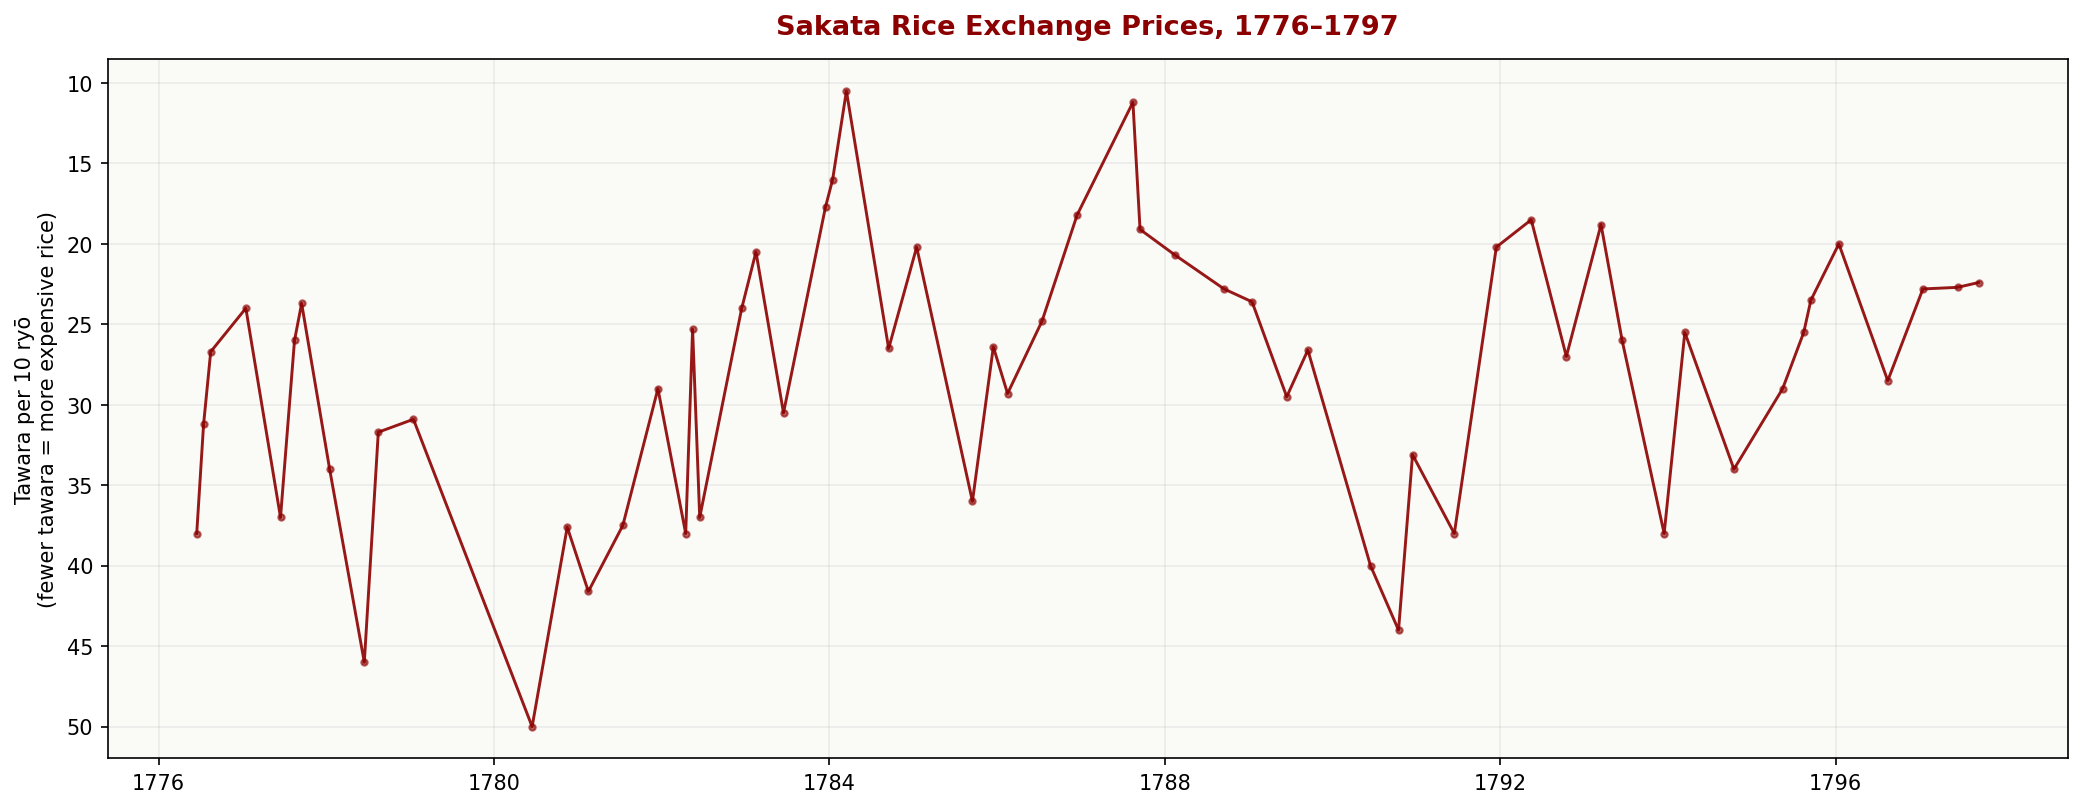
\includegraphics[width=\textwidth]{price_chart.png}
\caption{Sakata rice prices, An'ei 5 (1776) through Kansei 9 (1797),
reconstructed from the records in Article~85. The mean-reverting
character of the market is visible: prices oscillate within a bounded
range, with each spike followed by a return toward the center.}
\end{figure}

% --- An'ei 5 (1776) ---
\subsection*{An'ei 5, Year of the Monkey\hfill\normalfont\small\jp{安永五申年} (1776)}

Year-block direction: west (\jp{塞午}).
First-stem month: 5th month (\jp{五月甲}).
Autumn harvest: six-tenths crop (\jt{六分作}{rokubun-saku}).

\begin{description}[style=nextline, leftmargin=2em, font=\normalfont\bfseries]
\item[Opening] 38 tawara
\item[5th month (\textit{kinoe})] 31 tawara, 2 bu
\item[5th month] 26 tawara, 7 bu --- approximately 140-tawara rise
\item[6th month] 26 tawara, 7 bu --- 41-tawara decline
\item[12th month, 2nd day] 24 tawara --- \textit{kanoto} ceiling, 140-tawara rise
\end{description}

% --- An'ei 6 (1777) ---
\subsection*{An'ei 6, Year of the Rooster\hfill\normalfont\small\jp{安永六酉年} (1777)}

\begin{description}[style=nextline, leftmargin=2em, font=\normalfont\bfseries]
\item[Opening] 37 tawara
\item[6th month] 26 tawara
\item[7th month] 23 tawara, 7 bu
\item[Through 12th month] around 34 tawara
\end{description}

% --- An'ei 7 (1778) ---
\subsection*{An'ei 7, Year of the Dog\hfill\normalfont\small\jp{安永七戌年} (1778)}

Year-block direction: west (\jp{塞午}).
First-stem month: 11th month (\jp{十一月甲}).

\begin{description}[style=nextline, leftmargin=2em, font=\normalfont\bfseries]
\item[Opening] 46 tawara
\item[1st month] 31 tawara, 7 bu --- noted as ``sign of a \textit{kinoe} rise''
\item[1st month onward] A dispute arose at the certificate office (\jp{札方へ申分出}); 35 tawara, 5 bu. No settlement through the 10th month.
\item[11th month (\textit{kinoe})] 30 tawara, 9 bu --- ceiling on a \textit{fuj\=ojunichi}, 151-tawara rise
\end{description}

\textit{Following year, Year of the Boar:}
\begin{description}[style=nextline, leftmargin=2em, font=\normalfont\bfseries]
\item[6th month] 35 tawara, 5 bu --- 46-tawara decline
\end{description}

% --- An'ei 8 (1779) ---
\subsection*{An'ei 8, Year of the Boar\hfill\normalfont\small\jp{安永八亥年} (1779)}

Year-block direction: west (\jp{塞西}).

\begin{description}[style=nextline, leftmargin=2em, font=\normalfont\bfseries]
\item[Opening] 39 tawara to 44 tawara, 5 bu (range)
\item[Note] A dispute arose at the certificate office; no trading.
\end{description}

% --- An'ei 9 (1780) ---
\subsection*{An'ei 9, Year of the Rat\hfill\normalfont\small\jp{安永九子年} (1780)}

Year-block: west, rotating to Rooster (\jp{寒酉}).
First-stem month: 7th month (\jp{七月甲}).

This year's goods were plentiful; physical rice also at 50 tawara. New
certificates also opened at 50 tawara.

\begin{description}[style=nextline, leftmargin=2em, font=\normalfont\bfseries]
\item[9th month] 37 tawara, 6 bu
\end{description}

\textit{Following year, Year of the Ox:}
\begin{description}[style=nextline, leftmargin=2em, font=\normalfont\bfseries]
\item[1st month] 41 tawara, 6 bu
\item[5th month] 35 tawara, 9 bu --- ceiling on a \textit{hassen-k\=o}, 57-tawara rise
\end{description}

% --- Tenmei 1 (1781) ---
\subsection*{Tenmei 1, Year of the Ox\hfill\normalfont\small\jp{天明元丑年} (1781)}

Year-block: west (\jp{塞西}).
First-stem month: 5th month (\jp{五月甲}).

\begin{description}[style=nextline, leftmargin=2em, font=\normalfont\bfseries]
\item[5th month] 37 tawara, 5 bu
\item[10th month, 18th day] 29 tawara --- 188-tawara rise
\end{description}

\textit{Following year, Year of the Tiger:}
\begin{description}[style=nextline, leftmargin=2em, font=\normalfont\bfseries]
\item[3rd month] 38 tawara
\item[3rd month] 25 tawara, 3 bu --- \textit{kinoe} ceiling on an ordinary day, cumulative 127-tawara rise
\item[7th month] 25 tawara, 3 bu
\item[7th month] 27 tawara, 7 bu --- 24-tawara decline
\end{description}

% --- Tenmei 2 (1782) ---
\subsection*{Tenmei 2, Year of the Tiger\hfill\normalfont\small\jp{天明二寅年} (1782)}

Year-block: Rat direction (\jp{塞子}).
First-stem month: 3rd month (\jp{三月甲}).

\begin{description}[style=nextline, leftmargin=2em, font=\normalfont\bfseries]
\item[Opening] 37 tawara
\item[10th month] 24 tawara --- ceiling on a \textit{fuj\=ojunichi}, 130-tawara rise
\end{description}

\textit{Following year, Year of the Rabbit:}
\begin{description}[style=nextline, leftmargin=2em, font=\normalfont\bfseries]
\item[1st month] 20 tawara, 5 bu --- \textit{kinoe} ceiling, cumulative 33 tawara, 5 bu
\end{description}

% --- Tenmei 3 (1783) ---
\subsection*{Tenmei 3, Year of the Rabbit\hfill\normalfont\small\jp{天明三卯年} (1783)}

Year-block: Rat direction (\jp{塞子}).
First-stem month: 1st month (\jp{正月甲}).

\begin{description}[style=nextline, leftmargin=2em, font=\normalfont\bfseries]
\item[Opening] 30 tawara, 5 bu
\item[10th month] 17 tawara, 7 bu --- from 17.5 tawara
\item[12th month] 16 tawara
\end{description}

\textit{Following year, Year of the Dragon:}
\begin{description}[style=nextline, leftmargin=2em, font=\normalfont\bfseries]
\item[1st month, 2nd day] 12 tawara, 8 bu
\item[1st month, 26th day] 10 tawara, 5 bu --- \textit{hinoe} ceiling, 200-tawara rise
\item[7th month] 26 tawara, 5 bu --- 160-tawara decline
\end{description}

% --- Tenmei 4 (1784) ---
\subsection*{Tenmei 4, Year of the Dragon\hfill\normalfont\small\jp{天明四辰年} (1784)}

Year-block: blocked-Ox (\jp{塞子}).
First-stem month: 9th month (\jp{九月甲}).

\begin{description}[style=nextline, leftmargin=2em, font=\normalfont\bfseries]
\item[Opening] 32 tawara, 5 bu
\item[7th month (\textit{kinoe})] 20 tawara, 2 bu
\item[12th month] 20 tawara, 2 bu --- \textit{hinoto} ceiling, 123-tawara rise
\end{description}

% --- Tenmei 5 (1785) ---
\subsection*{Tenmei 5, Year of the Snake\hfill\normalfont\small\jp{天明五巳年} (1785)}

Year-block: blocked-Rabbit (\jp{塞卯}).
First-stem month: 7th month (\jp{七月甲}).

\begin{description}[style=nextline, leftmargin=2em, font=\normalfont\bfseries]
\item[7th month] 36 tawara
\item[10th month] 26 tawara, 4 bu --- \textit{ushi}-day \textit{hinoto} rise, 96-tawara rise
\item[12th month] 28 tawara, 8 bu
\end{description}

\textit{Following year, Year of the Horse:}
\begin{description}[style=nextline, leftmargin=2em, font=\normalfont\bfseries]
\item[1st month] 29 tawara, 3 bu
\item[5th month] 24 tawara, 8 bu --- \textit{ushi}-day \textit{kinoto} ceiling, total 116-tawara rise
\item[6th month] 24 tawara, 8 bu
\end{description}

% --- Tenmei 6 (1786) ---
\subsection*{Tenmei 6, Year of the Horse\hfill\normalfont\small\jp{天明六午年} (1786)}

Year-block: blocked-Rabbit (\jp{塞卯}).
First-stem month: 5th month (\jp{五月甲}).

\begin{description}[style=nextline, leftmargin=2em, font=\normalfont\bfseries]
\item[Opening] 30 tawara, 5 bu
\item[Same month] 18 tawara, 2 bu --- 5-tawara rise
\item[10th month] 18 tawara, 2 bu
\end{description}

\textit{Following year, Year of the Sheep:}
\begin{description}[style=nextline, leftmargin=2em, font=\normalfont\bfseries]
\item[6th month] 11 tawara, 2 bu --- \textit{fuj\=ojitsu}-day \textit{hinoto} ceiling, total 193-tawara rise
\item[Same month] 19 tawara, 1 bu --- 79-tawara decline
\end{description}

% --- Tenmei 7 (1787) ---
\subsection*{Tenmei 7, Year of the Sheep\hfill\normalfont\small\jp{天明七未年} (1787)}

Year-block: blocked-Rabbit (\jp{塞卯}).
First-stem month: 3rd month (\jp{三月甲}).

\begin{description}[style=nextline, leftmargin=2em, font=\normalfont\bfseries]
\item[Opening] 27 tawara
\end{description}

\textit{Following year, Year of the Monkey:}
\begin{description}[style=nextline, leftmargin=2em, font=\normalfont\bfseries]
\item[1st month] 20 tawara, 7 bu --- \textit{kinoe} ceiling, 63-tawara rise
\item[7th/8th month] 22 tawara, 8 bu
\item[9th month] 26 tawara
\end{description}

% --- Tenmei 8 (1788) ---
\subsection*{Tenmei 8, Year of the Monkey\hfill\normalfont\small\jp{天明八申年} (1788)}

Year-block: blocked-Horse (\jp{塞午}).
First-stem month: 1st month (\jp{正月甲}).

\begin{description}[style=nextline, leftmargin=2em, font=\normalfont\bfseries]
\item[Opening] 26 tawara
\item[11th month] 23 tawara, 6 bu --- \textit{ushi}-day \textit{kinoe} ceiling, 24-tawara rise
\end{description}

\textit{Following year, Year of the Rooster:}
\begin{description}[style=nextline, leftmargin=2em, font=\normalfont\bfseries]
\item[6th month] 40 tawara, 5 bu
\end{description}

% --- Tenmei 9 / Kansei 1 (1789) ---
\subsection*{Tenmei 9 / Kansei 1, Year of the Rooster\hfill\normalfont\small\jp{天明九酉年} (1789)}

Era changed to Kansei (\jp{寛政と改元}).
Year-block: blocked-Horse (\jp{塞午}).
First-stem month: 11th month (\jp{十一月甲}).

\begin{description}[style=nextline, leftmargin=2em, font=\normalfont\bfseries]
\item[Opening] 29 tawara, 5 bu
\item[7th month] 26 tawara, 6 bu
\item[Note] The record breaks off here.
\end{description}

% --- Kansei 2 (1790) ---
\subsection*{Kansei 2, Year of the Dog\hfill\normalfont\small\jp{寛政二戌年} (1790)}

Year-block: blocked-Horse (\jp{塞午}).
First-stem month: 7th month (\jp{七月甲}).

\begin{description}[style=nextline, leftmargin=2em, font=\normalfont\bfseries]
\item[New opening] 40 tawara
\item[8th month] 44 tawara
\item[10th month] 33 tawara, 1 bu --- \textit{kinoto} ceiling
\end{description}

% --- Kansei 3 (1791) ---
\subsection*{Kansei 3, Year of the Boar\hfill\normalfont\small\jp{寛政三亥年} (1791)}

Year-block: blocked-Rooster (\jp{塞酉}).
First-stem month: 5th month (\jp{五月甲}).

\begin{description}[style=nextline, leftmargin=2em, font=\normalfont\bfseries]
\item[Opening] 38 tawara --- from 27 tawara, 2 bu
\item[10th month] 20 tawara, 2 bu --- \textit{ten'ichi ten'j\=o}-day, 178-tawara rise
\item[12th month] 24 tawara
\end{description}

\textit{Following year, Year of the Rat:}
\begin{description}[style=nextline, leftmargin=2em, font=\normalfont\bfseries]
\item[3rd month, 16th day] 18 tawara, 5 bu --- 87-tawara decline
\item[6th month] 18 tawara, 9 bu --- 81-tawara decline
\item[8th month] 27 tawara --- rises again; 22 tawara
\end{description}

% --- Kansei 4 (1792) ---
\subsection*{Kansei 4, Year of the Rat\hfill\normalfont\small\jp{寛政四子年} (1792)}

Year-block: blocked-Rooster (\jp{塞酉}).
First-stem month: 3rd month (\jp{三月甲}).

\begin{description}[style=nextline, leftmargin=2em, font=\normalfont\bfseries]
\item[New opening] 32 tawara, 9 bu
\item[9th month] 22 tawara, 4 bu --- \textit{ten'ichi ten'j\=o} rise
\item[12th month] 23 tawara, 3 bu
\end{description}

\textit{Following year, Year of the Ox:}
\begin{description}[style=nextline, leftmargin=2em, font=\normalfont\bfseries]
\item[1st month, 17th day] 18 tawara, 8 bu --- \textit{kinoe} ceiling, total 148-tawara rise
\end{description}

% --- Kansei 5 (1793) ---
\subsection*{Kansei 5, Year of the Ox\hfill\normalfont\small\jp{寛政五丑年} (1793)}

Year-block: blocked-Rooster (\jp{塞酉}).
First-stem month: 1st month (\jp{正月甲}).

\begin{description}[style=nextline, leftmargin=2em, font=\normalfont\bfseries]
\item[New opening] 26 tawara
\item[Up to 10th month, 8th day] 38 tawara
\item[11th month] 31 tawara
\item[12th month] 30 tawara, 2 bu
\end{description}

\textit{Following year, Year of the Tiger:}
\begin{description}[style=nextline, leftmargin=2em, font=\normalfont\bfseries]
\item[1st month] 25 tawara, 5 bu --- \textit{ten'ichi ten'j\=o}-day \textit{hinoe} ceiling, 125-tawara rise
\item[6th month] 29 tawara
\item[8th month] 34 tawara --- 85-tawara decline
\end{description}

% --- Kansei 6 (1794) ---
\subsection*{Kansei 6, Year of the Tiger\hfill\normalfont\small\jp{寛政六寅年} (1794)}

Year-block: blocked-Rat (\jp{塞子}).
First-stem month: 9th month (\jp{九月甲}).

\begin{description}[style=nextline, leftmargin=2em, font=\normalfont\bfseries]
\item[New opening] 32 tawara
\item[8th month] 28 tawara, 3 bu
\end{description}

\textit{Following year, Year of the Rabbit:}
\begin{description}[style=nextline, leftmargin=2em, font=\normalfont\bfseries]
\item[Through 3rd month] Consolidation (\jp{持合})
\item[4th month onward] Around 29 tawara
\item[6th/7th month] Around 25 tawara, 5 bu --- \textit{kinoe} ceiling, approximately 65-tawara rise
\end{description}

% --- Kansei 7 (1795) ---
\subsection*{Kansei 7, Year of the Rabbit\hfill\normalfont\small\jp{寛政七卯年} (1795)}

Year-block: blocked-Rat (\jp{塞子}).
First-stem month: 7th month (\jp{七月甲}).

\begin{description}[style=nextline, leftmargin=2em, font=\normalfont\bfseries]
\item[New opening] 31 tawara
\item[7th month, 23rd day] 23 tawara, 5 bu --- \textit{ushi}-day \textit{tsuchinoe} ceiling, 128-tawara rise
\item[12th month] 20 tawara
\end{description}

\textit{Following year, Year of the Dragon:}
\begin{description}[style=nextline, leftmargin=2em, font=\normalfont\bfseries]
\item[1st--3rd month] From 19 tawara, around 20 tawara
\item[6th month, 22nd--23rd day] 28 tawara, 5 bu --- floor, 102-tawara decline
\item[Thereafter] Rises again to around 23.5 tawara
\end{description}

% --- Kansei 8 (1796) ---
\subsection*{Kansei 8, Year of the Dragon\hfill\normalfont\small\jp{寛政八辰年} (1796)}

Year-block: blocked-Rat (\jp{塞子}).
First-stem month: 5th month (\jp{五月甲}).

\begin{description}[style=nextline, leftmargin=2em, font=\normalfont\bfseries]
\item[Opening] 31 tawara, 4 bu
\item[11th month, 16th day] 22 tawara, 8 bu --- \textit{ushi}-day \textit{kanoe}, 87-tawara rise
\end{description}

\textit{Following year, Year of the Snake:}
\begin{description}[style=nextline, leftmargin=2em, font=\normalfont\bfseries]
\item[4th month, 29th day] 22 tawara, 7 bu --- 36-tawara decline
\item[7th month, 19th day] 22 tawara, 4 bu --- \textit{ushi}-day \textit{tsuchinoto} rise
\item[Intercalary 7th month] Record ends.
\end{description}

\bigskip

\begin{editorialnote}
The foregoing records the price movements of the Sakata rice exchange. In
the lower line, annotations such as ``\textit{kinoe} ceiling'' (\jp{甲天井})
or ``\textit{hinoe} ceiling'' (\jp{丙天井}) mean that the market reached its
ceiling in a \textit{kinoe}-month or a \textit{hinoe}-month, respectively.
The figures ``rise of one hundred and some-odd tawara'' (\jp{百何十俵上})
that follow are stated per 100 ry\=o of capital.
\end{editorialnote}

% =============================================================================
%  END OF LOWER VOLUME
% =============================================================================

\begin{center}
\rule{2in}{0.4pt}\\[1em]
{\small\itshape End of the Lower Volume}\\[0.3em]
{\small \jp{宗久翁相塲全集終}}
\end{center}


\end{document}
